\documentclass[12pt, twoside]{uosthesis}
%\usepackage[dvipsnames]{xcolor}
\usepackage{multirow}
\usepackage{amssymb}
\usepackage{titlesec}
\usepackage{amsmath}
\DeclareMathOperator{\arcsec}{arcsec}
\usepackage{float}
\usepackage{graphicx}
\usepackage{caption}
\usepackage{subfig}
\usepackage{graphicx}
\usepackage{xcolor}
\usepackage[round]{natbib}
\usepackage[section]{placeins}
\usepackage{mathrsfs}
\usepackage{bm}
\usepackage{stmaryrd}
\usepackage[utf8]{inputenc}
\usepackage{siunitx}
\usepackage{combelow}
\usepackage{afterpage}
\usepackage{xfrac}
\usepackage{ulem}       % To use \sout
\usepackage{enumitem}
\usepackage{epigraph}
\usepackage{pdflscape}

\usepackage{wrapfig}
\usepackage{lscape}
\usepackage{epstopdf}

\usepackage{rotfloat}
%\floatstyle{boxed} 
\restylefloat{figure}


\usepackage{geometry}
 \geometry{
 a4paper,
 left=40mm,
 right=30mm,
 top=30mm,
 bottom=30mm
 }

\definecolor{theblue}{HTML}{0000CD}

% disable this package for printed version
\usepackage[colorlinks=true, linktocpage=true, allcolors=theblue]{hyperref}

\titleformat{\chapter}[display]
  {\bfseries\Large}
  {\filright\MakeUppercase{\chaptertitlename} \Large\thechapter}
  {1ex}
  {}
  [\vspace{1ex} \hrule \vspace{1pt} \hrule]

\newcommand{\adv}{    {\it Adv. Space Res.}} 
\newcommand{\araa}{    {\it Annual Review of Astron and Astrophys.}} 
\newcommand{\annG}{   {\it Ann. Geophys.}} 
\newcommand{\aap}{    {\it Astron. Astrophys.}}
\newcommand{\aaps}{   {\it Astron. Astrophys. Suppl.}}
\newcommand{\aapr}{   {\it Astron. Astrophys. Rev.}}
\newcommand{\ag}{     {\it Ann. Geophys.}}
\newcommand{\aj}{     {\it Astron. J.}} 
\newcommand{\apj}{    {\it Astrophys. J.}}
\newcommand{\apjl}{   {\it Astrophys. J. Lett.}}
\newcommand{\apss}{   {\it Astrophys. Space Sci.}} 
\newcommand{\cjaa}{   {\it Chin. J. Astron. Astrophys.}} 
\newcommand{\gafd}{   {\it Geophys. Astrophys. Fluid Dyn.}}
\newcommand{\grl}{    {\it Geophys. Res. Lett.}}
\newcommand{\ijga}{   {\it Int. J. Geomagn. Aeron.}}
\newcommand{\jastp}{  {\it J. Atmos. Solar-Terr. Phys.}} 
\newcommand{\jgr}{    {\it J. Geophys. Res.}}
\newcommand{\mnras}{  {\it Mon. Not. Roy. Astron. Soc.}}
\newcommand{\na}{     {\it New Astronomy}}
\newcommand{\nat}{    {\it Nature}}
\newcommand{\pasp}{   {\it Pub. Astron. Soc. Pac.}}
\newcommand{\pasj}{   {\it Pub. Astron. Soc. Japan}}
\newcommand{\pre}{    {\it Phys. Rev. E}}
\newcommand{\solphys}{{\it Solar Phys.}}
\newcommand{\sovast}{ {\it Soviet  Astron.}} 
\newcommand{\ssr}{    {\it Space Sci. Rev.}}
\newcommand{\caa}{{\it Chinese Astron. Astrohpys.}} 
\newcommand{\apjs}{    {\it Astrophys. J. Suppl.}}
\newcommand{\zap}{   {\it Zeitschrift fuer Astrophysik}}

\newcommand{\bs}[1]{\boldsymbol{#1}}
\newcommand{\bn}{\boldsymbol{\nabla}}
\newcommand{\rgas}{\mathcal{R}}
\newcommand{\eref}[1]{Eq. \eqref{#1}}
\newcommand{\fref}[1]{Fig. \eqref{#1}}
\newcommand\encircle[1]{%
  \tikz[baseline=(X.base)] 
    \node (X) [draw, shape=circle, inner sep=0] {\strut #1};}
\newcommand{\Alfven}{Alfv\'{e}n } 
\newcommand{\Alfvenic}{Alfv\'{e}nic }
\newcommand{\size}{0.75}
\newcommand\measureISpecification{4ex}% not defined in mwe
\newcommand{\ctab}[1]{\raisebox{\dimexpr \measureISpecification/2 -.748ex}{#1}}% vertically centers numbers
\newcommand{\mfig}[4]{
  \begin{figure}
  \begin{center}
  \includegraphics[width=#1\linewidth]{#2}
  \caption{#3}
  \label{#4}
  \end{center}
  \end{figure}}
\newcommand{\kms}{~\rm{km ~s^{-1}}}
\newcommand{\kgm}{~\rm{kg ~m^{-3}}}
\newcommand{\np}{\\ \\}
%y amstext
\newcommand{\angstrom}{\textup{\AA}}
\newcommand{\degs}{^{\circ}}

\usepackage{enumitem}
\newlist{mylist}{itemize}{1}
\setlist[mylist]{label=\textbf{P1:}}
\newcommand\itemp{\item[\textbf{P2:}]}

\def\UrlFont{\sf}
\title{Numerical Magnetohydrodynamic Investigation of Jets in the Solar Atmosphere}   %note \\[1ex] is a line break in the title

\author{Fionnlagh Iain Mackenzie Dover}

\degree{Doctor of Philosophy}
\degreedate{April 2021}

\begin{document}

%this baselineskip gives sufficient line spacing for an examiner to easily
%markup the thesis with comments
\baselineskip=18pt plus1pt

%set the number of sectioning levels that get number and appear in the contents
\setcounter{secnumdepth}{3}
\setcounter{tocdepth}{3}

\maketitle

\afterpage{\null\newpage}
\begin{dedication}
In loving memory of Ewen Mackenzie and Colin Stoddart who both passed away during the course of the PhD. They are very much missed.  
\end{dedication}

\afterpage{\null\newpage}
\begin{acknowledgementslong}
Todo

\end{acknowledgementslong}

\afterpage{\null\newpage}
\begin{declaration}

I hereby declare that except where specific reference is made to the work of others, the contents of this dissertation are original and have not been submitted in whole or in part for consideration for any other degree or qualification in this, or any other university.
This dissertation is my own work and contains nothing which is the outcome of work done in collaboration with others, except as specified in the text and Acknowledgements.
This dissertation contains fewer than 80,000 words including appendices, bibliography, footnotes, tables and equations.

\begin{flushright}
Fionnlagh Iain Mackenzie Dover
\\
April 2021
\end{flushright}

\end{declaration}

\afterpage{\null\newpage}
\begin{abstract}
This thesis aims to increase our understanding of solar spicular jets. We carry out a series of numerical studies using MPI-AMRVAC to simulate jets in an idealised stratified solar atmosphere with a vertical uniform magnetic field. The jets are initiated  by driving them with a  momentum pulse. The relevance of multiple key parameters are investigated by varying the initial driver (amplitude, period, inclination with respect to magnetic field) and magnetic field conditions, to examine the parameter influence over the jet morphology and kinematics. We show the dynamics and morphology of simulated jets are sensitive to the key parameters. \np %
The simulated jets captured key observed spicule characteristics including maximum heights, field-aligned and non-field aligned mass motions/trajectories, and cross-sectional width deformations. The simulations mimic both the observed horizontal and transverse boundary deformation of the jet, which are under-reported in numerical studies. This may be due to the need for a very high spatial resolution to study this phenomenon. With the next generation of solar telescopes around the corner, more research will come to pass on the cross-sectional evolution of small-scale solar jets. Furthermore, the series simulations carried out and presented highlight the presence of not yet observed internal knot substructures generated by shock waves reflected within the jet beam. We show that these fine structures may not yet be observable, but they could be identified with new telescopes such as the Daniel K. Inoyue Solar Telescope (DKIST). If confirmed, these sub-structures will enable a new window through which observers could investigate the physics of spicular jets. This thesis embarks on highlighting the dynamics that may be observable with future facilities.
\end{abstract}

\afterpage{\null\newpage}
\begin{publications}

This Thesis is based on the following publications:

\begin{itemize}
\item Mackenzie Dover, F., Sharma, R., Kors{\'o}s, M. B., Erd\'elyi, R. (2020); Signatures of Cross-sectional Width Modulation in Solar Spicules due to Field-aligned Flows, \apj, Volume 905, Issue 1, \url{https://doi.org/10.3847/1538-4357/abc349}

\item Mackenzie Dover, F., Sharma, R., Erd\'elyi, R.; Magnetohydrodynamic Simulations of Spicular Jet Propagation Applied to Lower Solar Atmosphere Model, \apj, Volume 913, Issue 1, \url{https://doi.org/10.3847/1538-4357/abefd1}.
\end{itemize}

The following publication is not included in this Thesis:

\begin{itemize}
\item Mumford, S., et al. (2020); SunPy: A Python package for Solar Physics, The Journal of Open Source Software, Volume 5, Issue 46, \url{https://doi.org/10.21105/joss.01832}
\end{itemize}

\end{publications}

\begin{romanpages}          % start roman page numbering
\tableofcontents            % generate and include a table of contents
\listoffigures              % generate and include a list of figures
\end{romanpages}            % end roman page numbering

%now include the files of latex for each of the chapters etc

%------------------------------------------------------------------------------
\chapter{Introduction}
\label{chap:intro}
%------------------------------------------------------------------------------

%------------------------------------------------------------------------------
\section{Overview}
\label{sec:overview}
%------------------------------------------------------------------------------

The Sun has been an object of fascination and study for most of humanity's recorded history.
It is the main source of energy and accounts for most of the mass in the solar system.
The history of the Sun began approximately 4.6 billions years ago, with the gravitational collapse of a section of a massive molecular cloud \citep{Bouvier2010}.
This collapse created a protoplanetary disk with a protostar at its centre \citep{Montmerle2006}.
The protostar was composed of hydrogen, helium and lithium, which together accounted for around 98\% of its mass, while the other 2\% were heavier elements formed in younger generations of stars \citep{Zeilik1998}.
For approximately 50 million years after the formation of the protostar, it underwent a slow contraction which increased the temperature and pressure at its core, until it was able to start fusing hydrogen \citep{Yi2001}.
At that point the Sun became a main sequence star, which it will remain for at least another 5 billion years before becoming a red giant \citep{Schroder2008}.
It will subsequently become a red giant, and then a white dwarf, after having ejected nearly half of its mass \citep{Schroder2008}.
The ejected mass will form a planetary nebula, while the white dwarf will survive and may eventually become a hypothetical black dwarf \citep{Bloecker1995}.

The history of solar observations dates back to records of eclipses by Chinese astronomers as early as the year 2000 BCE \citep{Priest2014}.
\emph{Sunspots}, which are areas on the Sun's photosphere that are darker and cooler than their surroundings, have been recorded since at least 800 BCE by the Chinese, and 300 BCE by the ancient Greeks.
The first mention of the \emph{corona}, the high temperature atmosphere of the Sun, is attributed to the Byzantine scholar Leo Diaconus, as he observed the total eclipse of 22 December 968 from Constantinople, although people might have been aware of it as early as the time of Plutarch.
Solar \emph{prominences} were first described in the Russian First Chronicle of Novgorod as ``live embers" coming out of the Sun during the 1 May 1185 eclipse.
For a detailed account of pre-telescope astronomy, see \cite{Hetherington1996}.

\begin{figure}[t]
\centering
\includegraphics[width=\textwidth]{figures/butterfly_diagram.pdf}
\caption{The so-called \emph{butterfly diagram}, displaying the distribution of sunspots across latitudes over time.
Sunspots are most commonly found further from the equator at the beginning of the 11 year cycle, and closer to the equator near its end.
Credit: NASA Marshall Space Flight Center
}
\label{fig:butterfly}
\end{figure}

The advent of modern physics and astronomy led to great advances in solar physics in the past two centuries.
Some of the important discoveries that occurred during the 19\textsuperscript{th} century include the first description of the Sun's spectral lines by Fraunhofer, the discovery of the 11 year sunspot cycle by Schwabe (see Figure \ref{fig:butterfly}), and the first observations of solar flares and spicules by Carrington and Secchi, respectively.
The pace of discovery accelerated during the 20\textsuperscript{th} century, as new instruments, such as the coronagraph, were created, and the theory of \emph{magnetohydrodynamics} (MHD), which is used to describe many solar phenomena, was established.
Other important discoveries include the first description of the solar wind \citep{Parker1958} and the first observations of coronal mass ejections (CMEs).
Finally, our modern view of the Sun has been shaped by the multitude of solar missions that have become operational since the 1990s, such as Yohkoh, TRACE and SDO.
For a more detailed view of recent advances in solar physics, see, for example, \cite{Aschwanden2004, Priest2014}.

%------------------------------------------------------------------------------
\section{Structure and Physical Properties of the Sun}
\label{sec:structure}
%------------------------------------------------------------------------------

The Sun is a highly inhomogeneous nearly perfect sphere of plasma.
Its mean radius has been measured as being $R_\odot = 695.66$ \si{Mm} \citep{Haberreiter2008}, although the International Astronomical Union defines the nominal solar radius as $R_\odot^N = 695.7$ \si{Mm} \citep{Mamajek2015}.
It has a mass of $1.99 \times 10^{30}$ \si{kg} and loses around $1-1.5 \times 10^9$ \si{kg.s^{-1}} due to the solar wind \citep{Parker1958, Priest2014}.
The Sun is composed primarily of hydrogen (over 70\% of the solar mass), and helium (around 27\% of the solar mass), with only trace amounts of other elements, such as oxygen, carbon or nitrogen \citep{Lodders2003}.
The mean distance between the Sun and the Earth is one astronomical unit, defined as 1 \si{au} = \num{149597870700} \si{m}, or approximately $150 \times 10^6$ \si{km} \citep{Capitaine2012}.


In the following Subsections, we shall discuss the structure and physical properties of both the hidden solar interior, and of the visible atmosphere.
According to the latest models, the solar interior consists of four regions: the core, the radiative zone, the tachocline, and the convective zone, listed here from the innermost to the outermost.
The solar atmosphere is composed of the photosphere, chromosphere and corona.
While the solar atmosphere is observable with optical telescopes, due to the high density of solar plasma beneath the photosphere, the solar interior is opaque.
Our current knowledge of the interior is obtained through the mathematical models of helioseismology.

All of the structure described above, as well as some other phenomena that will be discussed later, has been visualised in Figure \ref{fig:sun}.
The majority of the current section has been adapted from \cite{Priest2014}, and should be considered a reference, unless a different reference is stated.

\begin{figure}[t]
\centering
\includegraphics[width=0.99\textwidth]{figures/Sun_structure.png}
\caption{The structure of the Sun. The core, radiative zone, tachocline and convective zone form the opaque inner layers, while the photosphere, chromosphere and corona form the observable atmosphere. Various observable phenomena, including a flare, prominence and photospheric granulation are also presented.
Adapted from Wikipedia.}
\label{fig:sun}
\end{figure}

%------------------------------------------------------------------------------
\subsection{The Solar Interior}
\label{subsec:interior}
%------------------------------------------------------------------------------

The \emph{solar core} extends from the center of the Sun to approximately 0.25 solar radii.
Its temperature is of the order of 15 million \si{K}, and its density around $1.6 \times 10^5$ \si{kg.m^{-3}}, which is enough to enable nuclear fusion.
The core contains approximately half the mass of the Sun in only 1/50 of its volume, and produces 99\% of its energy.
Most of this energy comes from two sets of fusion reactions: the proton-proton chain reaction and the CNO (carbon-nitrogen-oxygen) cycle.
Both of these reactions have the same outcome: four protons (\textsuperscript{1}H) become fused into one helium-4 nucleus (\textsuperscript{4}He), while other atoms only act as catalysts.
As a result of the process of fusion, some of the mass is converted into energy, and escapes in the form of high-energy $\gamma$-rays and also electron neutrinos.

The \emph{radiative zone} is the layer directly above the core, and extends from approximately $0.25 R_\odot$ to $0.7 R_\odot$.
The plasma composing this layer is opaque enough that the mean free path of photons travelling through it is of the order of $10^{-4}$ \si{m}.
If not for this opacity, photons would only take 2 \si{s} to cross the radiative zone, but instead they perform a random walk which lengthens their journey to \num{170000} years.
The numerous collisions that photons experience during this time have a major effect, that of increasing the wavelength of the high-energy $\gamma$-rays emerging from the core, to visible light at the solar surface.

In contrast to the radiative zone where energy is transported via radiative diffusion and thermal conduction, in the \emph{convective zone} the convective instability is the main source of energy transport.
These two sections are separated by a thin shear layer, called the \emph{tachocline} \citep{Spiegel1992}, which is likely significant in the generation of the global solar magnetic field.
The convective zone is the last of the interior layers and extends from around $0.7 R_\odot$ to $1 R_\odot$.

%------------------------------------------------------------------------------
\subsection{The Solar Atmosphere}
\label{subsec:atmosphere}
%------------------------------------------------------------------------------

The solar atmosphere may be divided into four regions which have different physical characteristics (see Figure \ref{fig:sun}).
The lowest of these, the \emph{photosphere}, is the Sun's surface layer and is only around 500 \si{km} thick.
It is where most of the Sun's visible light is emitted.
Most of the photosphere is composed of granules with hot bright centres of rising plasma and cool dark boundaries.
This granulation is caused by turbulent convective motion lifting hot plasma, which subsequently cools and falls, forming the granular boundaries, called intergranular lanes.
Regions of strong magnetic flux may inhibit this convection, and form sunspots.
Granules have diameters ranging from 0.3 to 2 \si{Mm}, and lifetimes of 1 to 20 minutes, with typical values of 5 to 8 minutes \citep{Priest2014}.

The \emph{chromosphere} extends over the photosphere and exhibits various forms of structuring.
The most common of these are spicules, which are dynamic jets that cover the solar surface and form a sort of canopy.

\begin{figure}[h]
\centering
\includegraphics[width=0.8\textwidth]{figures/VAL.png}
\caption{The mean variation of the density and temperature, as described by the VAL  model. Image credit: \cite{Avrett2008}.
}
\label{fig:val}
\end{figure}

The \emph{corona} is the outermost regions of the Sun's atmosphere, separated from the chromosphere by a narrow \emph{transition region}, and extends outwards into the solar wind.
Significant structuring is present in the corona due to the intense magnetic fields that permeate it.
Of particular interest in this Thesis are \emph{coronal loops}.
They are a common form of structuring, comprising of hot plasma (2 to 3 \si{MK}) frozen into the magnetic fields tied to the photosphere.
Coronal loops are waveguides for MHD waves of various modes, an aspect which we examine in Chapter 3 of this Thesis.
Other structures in the corona include coronal holes, X-ray bright points, and coronal streamers.

Coronal mass ejections are large-scale releases of solar plasma from the corona, often following solar flares or prominence eruptions.
Their bulk speeds take a wide range of values, from less than 100 \si{km.s^{-1}} to over 2000 \si{km.s^{-1}}.
They account for approximately 5 to 10 per cent of the solar wind mass-loss.
It is shown in Chapter 2 that the high bulk speed of CMEs makes them particularly prone to the Kelvin-Helmholtz instability.

The mean temperatures and densities of the regions introduced above are commonly described using the VAL (Vernazza-Avrett-Loeset) model \citep{Vernazza1981, Avrett2008}.
According to this model, the density suffers a decrease from approximately $10^{-4}$ \si{kg.m^{-3}} at the base of the photosphere to around $10^{-10}$ \si{kg.m^{-3}} at the transition region, and then falls steeply to almost $10^{-12}$ \si{kg.m^{-3}} in the corona.
The temperature also rises dramatically across the transition region, from a chromospheric value of \num{25000} to over 1 \si{MK} in the corona.
The mechanisms that cause this abrupt increase in temperature are still not well understood, and are a topic of ongoing study.

%------------------------------------------------------------------------------
\section{Equations of Magnetohydrodynamics}
\label{sec:mhdeqns}
%------------------------------------------------------------------------------

In Section \ref{sec:structure} we described some of the main physical properties of the Sun, gave an overview of its large- and small-scale structure, and introduced a number of solar phenomena.
In order to mathematically model this phenomena, we need to employ a suitable framework.
Due to the fact that, in this Thesis, we are mainly concerned with phenomena in the corona, we considered the most appropriate framework the equations of \emph{ideal magnetohydrodynamics} (MHD).

In this Section, we give a brief description of how the ideal MHD equations are obtained, and we motivate their use in modelling coronal phenomena.
The MHD equations may be obtained using two different methods:
\begin{itemize}
\item Averaging the kinetic equations for plasmas;
\item Combining Maxwell's equations for electric and magnetic fields with the fluid equations.
\end{itemize}
The first of these methods is mathematically more complicated and shall be omitted in this section.
However, the relevant derivation may be found in classical works such as \cite{Braginskii1965} or \cite{Chapman1970}, or more modern introductions to MHD, such as \cite{Goossens2003} or \cite{Goedbloed2004}.

For the second, we require the equations of Maxwell, that describe the evolution of the electric field, $\mathbf E(\mathbf{r}, t)$ (measured in \si{V.m^{-1}}), and magnetic field $\mathbf B(\mathbf{r}, t)$ (measured in \si{T}), in response to the current density $\mathbf j(\mathbf{r}, t)$ (measured in \si{A.m^{-2}}) and the total electric charge density $\mathbf \tau(\mathbf{r}, t)$ (measured in \si{C.m^{-3}}).
Additionally, we require the equations of conservation of momentum, mass, and energy, which govern the dynamical evolution of the density, $\rho(\mathbf{r}, t)$ (measured in \si{kg.m^{-3}}), pressure $p(\mathbf{r}, t)$ (measured in \si{N.m^{-2}}), and velocity, $\mathbf{v}(\mathbf{r}, t)$ (measured in \si{m.s^{-1}}), of a fluid.
Here, $\mathbf{r}$ is the position vector, and $t$ is time (measured in \si{s}).

After making a number of simplifying assumptions, we combine these two systems of equations in order to eliminate, $\mathbf{E}, \mathbf{j}$, and $\tau$, and obtain a system of coupled equations in terms of $\mathbf{v}, \mathbf{B}, \rho$, and $p$.

%------------------------------------------------------------------------------
\subsection{Assumptions of Ideal MHD}
\label{subsec:assumpt}
%------------------------------------------------------------------------------

The MHD equations describe the macroscopic dynamics of magnetised plasmas.
As such, we need to establish under what conditions kinetic effects, i.e. small scale effects, stop becoming significant, and the plasma may be treated as a bulk fluid.
This Subsection is based on \cite{Goedbloed2004} and \cite{Priest2014}.

We begin by assuming that the model plasma is \textit{electrically neutral}, which is true for most applications in the solar photosphere and corona.
We define the number densities of positive and negative particles per unit volume, $n_+$ and $n_-$, respectively, and the total number density per unit volume, $n$.
It follows that, for charge neutrality, we require
$
|n_+ - n_-| \ll n.
$
The absence of charge neutrality is called a \textit{charge imbalance}, and such an imbalance produces an electric field with a spatial range of the \textit{Debye length} \citep[see, for example,][]{Boyd2003},
%
\begin{equation}
\label{eq:ass2}
\lambda_D = \sqrt{\frac{\varepsilon_0 k_B T}{n q}}.
\end{equation}
%
The quantities in Equation \eqref{eq:ass2} are defined as follows.
The electric constant, $\varepsilon_0$, also called the permittivity of free space, may be written as
%
\begin{equation}
\label{eq:electricconst}
\varepsilon_0 = \frac{1}{\mu_0 c^2} \approx 8.854187817... \times 10^{-12} \: \si{F.s^{-1}},
\end{equation}
%
where, $\mu_0$ is the magnetic permeability of free space, defined as
%
\begin{equation}
\label{eq:magneticconst}
\mu_0 = 4 \pi \times 10^7 \: \si{N.A^{-2}},
\end{equation}
%
and $c = \num{299792458} \: \si{m.s^{-1}}$ is the speed of light.
$k_B \approx 1.38 \times 10^{-23} \: \si{J.K^{-1}}$ is the Boltzmann constant, and $q$ is the charge of a particle.
We may now define a plasma as a collection of charge particles whose number density, $n$, is very large in a sphere of radius $\lambda_D$,
%
\begin{equation}
\label{eq:debye}
\frac{4}{3} \pi \lambda_D^3 n \gg 1.
\end{equation}
%
Typical values of the Debye length are of the order of $10^{-3}$ \si{m} in the corona, $10^{-11}$ \si{m} in the solar core, and $10$ \si{m} in the solar wind.

The second assumption we must make is that the plasma may be treated as a continuum.
This is valid provided the length-scales of gradients in the plasma are much greater than characteristic plasma lengths, such as the gyroradius (also called the Larmor radius or cyclotron radius), which is defined as
\[
r_g = \frac{m v_\perp}{|q| B}.
\]
Here, $m$ is the mass of the particle, $v_\perp$ is the component of the velocity perpendicular to the magnetic field, and $q$ is the electric charge of the particle.
Furthermore, we assume that the plasma is in thermodynamic equilibrium, such that its distribution function is close to Maxwellian.
This assumption is true for time scales much greater than the collision times, and length scales much greater than the mean free path of the plasma.
The mean free path in the ambient corona may be up to 1 \si{km} due to the low particle density of the plasma.

We also assume that we may treat the plasma as a single fluid.
This is a good approximation for applications to the photosphere and corona, but may not be accurate for models of the chromosphere since interactions between ions and neutrals are significant in that region.

We also assume that the equations are formulated for an inertial frame, and that the typical plasma velocity is non-relativistic.
We may write this second condition as
$
v_0 \ll c,
$
where $v_0$ is the typical speed of the plasma.

Note that, in this Thesis, we only consider adiabatic, inviscid, and ideal plasmas, so that we may neglect any terms related to heat transfer, viscosity and resistivity, when deriving the ideal MHD equations.

Finally, we note that all equations shall be considered in their differential form in \si{m.k.s} units.

%------------------------------------------------------------------------------
\subsection{Maxwell's Equations}
\label{subsec:Max}
%------------------------------------------------------------------------------

We begin by considering the first of Maxwell's equations of classical electrodynamics, which is Gauss's law for the electric field,
%
\begin{equation}
\label{eq:max1}
\nabla \cdot \mathbf E = \dfrac{\tau}{\varepsilon_0}.
\end{equation}
%
This states that the divergence of the electric field is equal to the total electric charge density divided by the electric constant, $\varepsilon_0$, defined in Equation \eqref{eq:electricconst}.

The second equation is the condition that there exist no magnetic monopoles.
This equation is also known as Gauss's law for magnetism, and may be written as
%
\begin{equation}
\label{eq:max2}
\nabla \cdot \mathbf B = 0.
\end{equation}
%
Equation \eqref{eq:max2} states that magnetic fields must be solenoidal vector fields.
As a consequence, point charges of magnetic field, analogous to electric charges, may not exist.

The third equation is the Maxwell-Faraday equation,
%
\begin{equation}
\label{eq:max3}
\nabla \times \mathbf E = - \frac{\partial \mathbf B}{\partial t},
\end{equation}
%
which states that any change of the magnetic field in time, will coincide with a spatially varying non-conservative electric field, and vice-versa.
A straightforward example of this concept is that of the generation of electric current in a dynamo using a permanent magnet, such as a bar magnet.
In such an instrument, a rotating magnet surrounded by coils of wire, creates electric current in the wires.

The final equation is known as Amp\`ere's circuital law,
%
\begin{equation}
\label{eq:max4}
\nabla \times \mathbf B = \mu_0 \mathbf j + \frac{1}{c^2} \frac{\partial \mathbf E}{\partial t},
\end{equation}
%
which states that magnetic fields may be generated through both an induced electric current, and a change in the electric field.
Only the first mechanism was originally included in Amp\`ere's law, while the second mechanism is due to Maxwell.
It follows from Equations \eqref{eq:max3} and \eqref{eq:max4} that time-varying electric and magnetic fields will generate spatially varying magnetic and electric fields, respectively.

%------------------------------------------------------------------------------
\subsection{Equations of Gas Dynamics}
\label{subsec:gas}
%------------------------------------------------------------------------------

Having introduced Maxwell's equations, \eqref{eq:max1} -- \eqref{eq:max4}, we now wish to introduce the equations governing the dynamical evolution of the density, $\rho(\mathbf{r}, t)$, pressure $p(\mathbf{r}, t)$, and velocity $\mathbf{v}(\mathbf{r}, t)$ of a plasma.
Before we proceed, we must introduce the Lagrangian time-derivative of a fluid,
%
\begin{equation}
\label{eq:lagder1}
\frac{\mathrm{D}}{\mathrm{D} t} = \frac{\partial}{\partial t} + \mathbf{v} \cdot \nabla
\end{equation}
%
which is evaluated in the frame of reference of a moving fluid, and differs from the Eulerian time-derivative, $\partial / \partial t$, which is evaluated at a fixed point.

Since we are only concerned with ideal MHD, we only consider the equations of conservation of mass, momentum and energy of adiabatic and inviscid plasmas.
The equation for the evolution of the density, most conveniently written
%
\begin{equation}
\label{eq:mass}
\frac{\mathrm{D} \rho}{\mathrm{D} t} + \rho \nabla \cdot \mathbf{v} = 0,
\end{equation}
%
is called the mass continuity equation, and may also be written
%
\begin{equation}
\label{eq:gas1-1}
\frac{\partial \rho}{\partial t} + \nabla \cdot ( \rho \mathbf{v} ) = 0.
\end{equation}
%
In this form, we can see that it represents conservation of mass, since an increase in density at a point, represented by a positive $\partial \rho / \partial t$, is accompanied by mass flowing in, i.e. $\nabla \cdot ( \rho \mathbf{v} ) < 0$.

We introduce the energy equation, which may be written in terms of the internal energy per unit mass, $e$ (measured in \si{J.kg^{-1}}),
%
\begin{equation}
\label{eq:gas2}
\rho \frac{\mathrm{D} e}{\mathrm{D} t} - \frac{p}{\rho} \frac{\mathrm{D} \rho}{\mathrm{D} t} = - \mathcal{L},
\end{equation}
%
where $\mathcal{L}$ is the energy loss function (measured in \si{J.m^{-3}.s^{-1}}).
Since we are only considering adiabatic processes, the energy gains and losses balance, so that $\mathcal{L} \equiv 0$, and Equation \eqref{eq:gas2} may be written as
%
\begin{equation}
\label{eq:gas2-1}
\rho \frac{\mathrm{D} e}{\mathrm{D} t} - \frac{p}{\rho} \frac{\mathrm{D} \rho}{\mathrm{D} t} = 0,
\end{equation}
%
such that energy is conserved.
In order to further simplify Equation \eqref{eq:gas2-1}, we wish to eliminate the internal energy and obtain an equation relating the pressure and density.
The plasma pressure is determined by an equation of state, which we assume to be the ideal gas law,
%
\begin{equation}
\label{eq:gas2-2}
p = \frac{k_B}{m} \rho T,
\end{equation}
%
where $m$ is the mean mass (measured in \si{kg}) of the particles that make up the plasma, and $T$ is the absolute temperature of the plasma (measured in \si{K}).
For an ideal gas, the heat capacity is constant with temperature, and we may write the internal energy as 
%
\begin{equation}
\label{eq:gas2-3}
e = c_v T,
\end{equation}
%
where $c_v$ is the specific heat at constant volume.
We define the specific heat at constant pressure as
%
\begin{equation}
\label{eq:gas2-4}
c_p = c_v + \frac{k_B}{m},
\end{equation}
%
and the ratio of specific heats (also called the adiabatic index),
%
\begin{equation}
\label{eq:gas2-5}
\gamma = \frac{c_v}{c_p}.
\end{equation}
%
We may write the specific heat at constant volume as
%
\begin{equation}
\label{eq:gas2-6}
c_v = \frac{1}{\gamma - 1} \frac{k_B}{m},
\end{equation}
%
and combine Equations \eqref{eq:gas2-2}, \eqref{eq:gas2-3}, and \eqref{eq:gas2-6} to obtain
%
\begin{equation}
\label{eq:gas2-7}
e = \frac{1}{\gamma - 1} \frac{p}{\rho}.
\end{equation}
%
We substitute \eqref{eq:gas2-7} into \eqref{eq:gas2-1} to obtain the desired form of the energy equation,
%
\begin{equation}
\label{eq:energy}
\frac{\mathrm{D} p}{\mathrm{D} t} - \frac{\gamma p}{\rho} \frac{\mathrm{D} \rho}{\mathrm{D} t} = 0.
\end{equation}
%
It is worth noting that, the adiabatic index is related to the number of degrees of freedom of a molecule by $\gamma = 1 + 2/f$, where $f$ is the number of degrees of freedom.
Since, in this Thesis, we are primarily concerned with fully ionised monoatomic plasmas characteristic of the solar corona, we may assume that $f = 3$, and $\gamma = 5/3$.

The final equation of gas dynamics is the equation of motion for a fluid element, which connects the equations of electrodynamics, described in Subsection \ref{subsec:Max}, with the gas dynamics equations described in the current section.
In order for conservation of momentum to be satisfied, we require
%
\begin{equation}
\label{eq:gas3}
\rho \frac{\mathrm{D} \mathbf v}{\mathrm{D} t} = \mathbf{F},
\end{equation}
%
where $\mathbf{F}$ (measured in units of force density, \si{N.m^{-3}}) is given by
%
\begin{equation}
\label{eq:gas3-1}
\mathbf{F} \equiv - \nabla p + \rho \mathbf{g} + \mathbf{j} \times \mathbf{B} + \tau \mathbf{E}.
\end{equation}
%

%------------------------------------------------------------------------------
\subsection{The Equations of Ideal MHD}
\label{subsec:mhdderiv}
%------------------------------------------------------------------------------

In order to connect the equations of electrodynamics, described in Subsection \ref{subsec:Max}, with the equations of gas dynamics described in Subsection \ref{subsec:gas}, we begin by introducing Ohm's law, which links the electric, magnetic and velocity fields via the current density, such that
%
\begin{equation}
\label{eq:ohm1}
\mathbf{E} + \mathbf{v} \times \mathbf{B} = \eta \mathbf{j},
\end{equation}
%
where $\eta$ is the electrical resistivity (measured in $\si{\Omega.m}$).
In this Thesis, we are not concerned with situations where non-ideal effects, such as resistivity, play an important role.
As such, we may set $\eta = 0$, and Ohm's law reduces to
%
\begin{equation}
\label{eq:ohm2}
\mathbf{E} + \mathbf{v} \times \mathbf{B} = 0.
\end{equation}
%
From Equation \eqref{eq:ohm2}, we see that the typical scales of the magnitude of the electric field, $E$, and magnetic field, $B$, satisfy
%
\begin{equation}
\label{eq:scales1}
E \sim - v B.
\end{equation}
%

We now return to Equation \eqref{eq:max4}, and find that
%
\begin{equation}
\label{eq:scales2}
\frac{1}{c^2} \left| \frac{\partial \mathbf{E}}{\partial t} \right|
\sim \frac{v}{c^2} \frac{B}{t_0}
= \frac{v^2}{c^2} \frac{B}{l_0}
= \mathcal{O}(v^2/c^2),
\end{equation}
%
where $t_0$ and $l_0$ are the characteristic time and length scales.
Here, $\mathcal{O}$, represents the order of a quantity, and is known as Big $\mathcal{O}$ notation.
The quantity in Equation \eqref{eq:scales2} is much smaller than the term on the LHS of Equation \eqref{eq:max4}, which is $|\nabla \times \mathbf{B}| \sim B / l_0$.
It follows that the term in Equation \eqref{eq:scales2} may be neglected from Equation \eqref{eq:max4}, and we recover the original form of Amp\`ere's law,
%
\begin{equation}
\label{eq:ampere}
\mathbf j = \frac{1}{\mu_0} \nabla \times \mathbf B.
\end{equation}
%

The equation of motion, \eqref{eq:gas3}, is also simplified by the assumption of non-relativistic velocities.
Using Equations \eqref{eq:max1} and \eqref{eq:scales1}, we find that the electrostatic acceleration satisfies
%
\begin{equation}
\label{eq:scales3}
\tau |\mathbf{E}| \sim \frac{v B}{\mu_0 c^2 l_0} \times v B
= \frac{v^2}{c^2} \frac{B^2}{\mu_0 l_0}
= \mathcal{O}(v^2/c^2).
\end{equation}
%
Using Equation \eqref{eq:ampere}, we find that $\tau |\mathbf{E}| \ll |\mathbf{j} \times \mathbf{B}| \sim B^2 / \mu_0 l_0$.
This means that the final term in Equation \eqref{eq:gas3-1} may be neglected, and the equation of motion becomes
%
\begin{equation}
\label{eq:momentum}
\rho \frac{\mathrm{D} \mathbf v}{\mathrm{D} t} = - \nabla p + \rho \mathbf{g} + \mathbf{j} \times \mathbf{B},
\end{equation}
%

Finally, we combine Equations \eqref{eq:max3} and \eqref{eq:ohm2} to obtain the induction equation,
%
\begin{equation}
\label{eq:induction}
\frac{\partial \mathbf{B}}{\partial t} - \nabla \times ( \mathbf{v} \times \mathbf{B} ) = 0.
\end{equation}
%
We have, thus, obtained a system of 8 coupled partial differential equations, Equations \eqref{eq:mass}, \eqref{eq:energy}, \eqref{eq:momentum}, and \eqref{eq:induction}, which constitute the system of ideal MHD equations.
Equation \eqref{eq:max2}, the condition that there are no magnetic monopoles, is also part of this system, but is always satisfied if it is satisfied as an initial condition.
We can see this if we take the divergence, $\nabla \cdot$, of Equation \eqref{eq:induction}.

%------------------------------------------------------------------------------
\subsection{Consequences of Ideal MHD}
\label{subsec:conseq}
%------------------------------------------------------------------------------

%The first observation we need to make concerns the conservation of the quantities described by the ideal MHD equations.
%Equations \eqref{eq:mass}, \eqref{eq:energy}, \eqref{eq:momentum}, and \eqref{eq:induction} may be written in such a form that it becomes obvious that mass, energy, momentum, and the magnetic field, respectively, are conserved \citep{Goedbloed2004}.

A first remark on the ideal MHD equations comes from the momentum equation, \eqref{eq:momentum}, where the term $\mathbf{j} \times \mathbf{B}$, called the \textit{Lorentz force}, may be written as
%
\begin{equation}
\label{eq:lorentz}
\mathbf{j} \times \mathbf{B}
= \frac{1}{\mu_0} ( \nabla \times \mathbf B ) \times \mathbf{B}
= \frac{ ( \mathbf{B} \cdot \nabla ) \mathbf{B}}{\mu_0}
- \nabla \left( \frac{\mathbf{B}^2}{2 \mu_0} \right).
\end{equation}
%
The first term on the right-hand side is called the \textit{magnetic tension} force, while the second is the \textit{magnetic pressure} force.
It may be shown that the magnetic tension results in a negative stress in a direction parallel to $\mathbf{B}$, while the magnetic pressure causes a positive stress normal to $\mathbf{B}$ \citep{Goedbloed2004}.

A second result of note is Alfv\'en's frozen flux theorem, which states that, in ideal MHD, magnetic flux is conserved so that the magnetic field moves with the plasma.
This is in addition to the quantities that we already know are conserved, from the Euler equations, namely mass, energy and momentum.

While the ideal MHD equations have various other properties, we restrict our discussion to the two above, as they are most relevant in this Thesis.


%------------------------------------------------------------------------------
\subsection{The Linear Ideal MHD Equations}
\label{subsec:linearmhd}
%------------------------------------------------------------------------------

The nonlinear form of the MHD Equations is difficult to treat analytically in most situations.
For many applications, we may \textit{linearise} Equations \eqref{eq:mass}, \eqref{eq:energy}, \eqref{eq:momentum}, and \eqref{eq:induction} in the following way.
We assume that the dependent variables, $\mathbf{v}, \mathbf{B}, \rho$ and $p$, may be split into two distinct quantities: a \textit{background} (or \textit{equilibrium}) value, and a small \textit{perturbation}.
We write this as
%
\begin{align}
\begin{split}
\label{eq:perturbations}
\mathbf{v} & = \mathbf{v_0} + \mathbf{v'},
\qquad
\mathbf{B} = \mathbf{B_0} + \mathbf{b'},
\\
\rho & = \rho_0 + \rho',
\qquad
p = p_0 + p',
\end{split}
\end{align}
%
where the subscript $0$ represents the background value, and the apostrophe denotes the perturbation.
We assume that the perturbations of the magnetic field, density and pressure are much smaller than their equilibrium values, i.e.
%
\begin{equation}
| \mathbf{B_0} | \gg | \mathbf{b'} |,
\qquad
\rho_0 \gg \rho',
\qquad
p_0 \gg p'.
\end{equation}
%
This assumption is not always applicable to the velocity perturbation since the background flow may be zero ($\mathbf{v_0} = \mathbf 0$).
In such cases, we say that the velocity perturbation is much smaller than some other characteristic speed of the system, such as the local speed of sound,
%
\begin{equation}
\label{eq:soundspeed}
c_s = \sqrt{ \gamma \frac{p_0}{\rho_0} },
\end{equation}
%
or Alfv\'en speed
%
\begin{equation}
\label{eq:alfvenspeed}
v_A = \sqrt{ \frac{B_0^2}{\mu_0 \rho} }.
\end{equation}
%
It is worth noting that the background quantities may be inhomogeneous spatially and may evolve temporally.

We, now, insert Equations \eqref{eq:perturbations} into Equations \eqref{eq:mass}, \eqref{eq:energy}, \eqref{eq:momentum}, and \eqref{eq:induction}, and neglect nonlinear coupling due to products of perturbations.
This yields the system of linear ideal MHD equations
%
\begin{align}
\label{eq:masslin}
& \frac{\mathrm{D} \rho'}{\mathrm{D} t}
+ \rho_0 \nabla \cdot \mathbf{v'}
= 0,
\\[0.2cm]
\label{eq:enerlin}
& \frac{\mathrm{D} p'}{\mathrm{D} t}
= c_s^2 \frac{\mathrm{D} \rho'}{\mathrm{D} t},
\\[0.2cm]
\label{eq:momlin}
\rho_0 & \frac{\mathrm{D} \mathbf v'}{\mathrm{D} t}
= - \nabla p'
+ \frac{1}{\mu_0} (\nabla \times \mathbf{b'}) \times \mathbf{B_0},
\\[0.2cm]
\label{eq:indlin}
& \frac{\partial \mathbf{b'}}{\partial t}
= \nabla \times (\mathbf{v_0} \times \mathbf{b'})
+ \nabla \times (\mathbf{v'} \times \mathbf{B_0}),
\\[0.2cm]
\nonumber
& \nabla \cdot \mathbf{b}' = 0,
\end{align}
%
where the Lagrangian derivative is now defined as
%
\begin{equation}
\label{eq:lagder2}
\frac{\mathrm{D}}{\mathrm{D} t}
= \frac{\partial}{\partial t}
+ \mathbf{v_0} \cdot \nabla,
\end{equation}
%
and the apostrophe was dropped when writing the perturbations.
In deriving Equations \eqref{eq:masslin} - \eqref{eq:indlin}, we have neglected gravity, since the models we derive in this Thesis have applications to small-scale phenomena, where gravity does not have a strong effect.
We also assumed that $\mathbf{B_0}, \rho_0$ and $p_0$ are spatially homogeneous in each layer, and do not evolve temporally (i.e. independent of $\mathbf{r}$ and $t$), and $\mathbf{v_0}$ is homogeneous in space in each layer (i.e. independent of $\mathbf{r}$).
These assumptions are not true in general, but are sufficient for the analyses in this Thesis.

%------------------------------------------------------------------------------
\subsection{Equations of Incompressible Ideal MHD}
\label{subsec:inc-mhd}
%------------------------------------------------------------------------------

A special form of the ideal MHD equations, which we will make use of later in this Thesis, assumes that all motion is incompressible.
We define incompressibility as the property that density is constant in a fluid, such that the MHD Equations (neglecting gravity) are reduced to
%
\begin{align}
\label{eq:mominc}
\frac{\mathrm{D} \mathbf v}{\mathrm{D} t}
& = - \frac{1}{\rho} \nabla p_T
+ \frac{1}{\mu_0 \rho} ( \mathbf{B} \cdot \nabla ) \mathbf{B},
\\[0.2cm]
\label{eq:indinc}
\frac{\mathrm{D} \mathbf B}{\mathrm{D} t}
& = ( \mathbf{B} \cdot \nabla ) \mathbf{v},
\\[0.2cm]
\label{eq:divv}
\nabla \cdot \mathbf{v} & = 0,
\\[0.1cm]
\nonumber
\nabla \cdot \mathbf{B} & = 0,
\end{align}
%
where $p_T$ is the total (gas plus magnetic) pressure, and the Lagrangian derivative is given by Equation \eqref{eq:lagder1}.

Following the method described in Subsection \ref{subsec:linearmhd}, we linearise Equations \eqref{eq:mominc} - \eqref{eq:divv}, and obtain
%
\begin{align}
\label{eq:mominclin}
\frac{\mathrm{D} \mathbf v'}{\mathrm{D} t}
& = - \frac{1}{\rho_0} \nabla p_T'
+ \frac{1}{\mu_0 \rho_0} ( \mathbf{B_0} \cdot \nabla ) \mathbf{b'},
\\[0.2cm]
\label{eq:indinclin}
\frac{\mathrm{D} \mathbf b'}{\mathrm{D} t}
& = ( \mathbf{B_0} \cdot \nabla ) \mathbf{v'},
\\[0.2cm]
\label{eq:divvlin}
\nabla \cdot \mathbf{v'} & = 0,
\\[0.1cm]
\nonumber
\nabla \cdot \mathbf{b}' & = 0,
\end{align}
%
where $p_T'$ is the perturbation of the total pressure, and the Lagrangian derivative is given by Equation \eqref{eq:lagder2}.
As in Subsection \ref{subsec:linearmhd}, we have assumed that the background quantities are spatially homogeneous, and $\mathbf{B_0}$ is also independent of $t$.

We now introduce the plasma displacement, $\bm \xi (\mathbf{r}, t)$, which is related to the velocity by
%
\begin{equation}
\label{eq:xi}
\mathbf{v'}
= \frac{\mathrm{D} \bm \xi}{\mathrm{D} t}
= \frac{\partial}{\partial t}
+ ( \mathbf{v_0} \cdot \nabla ) \bm \xi.
\end{equation}
%
Substituting Equation \eqref{eq:xi} into Equation \eqref{eq:divvlin}, we obtain
%
\begin{equation}
\frac{\mathrm{D}}{\mathrm{D} t} ( \nabla \cdot \bm \xi ) = 0,
\end{equation}
%
since $\mathbf{v_0}$ is independent of $\mathbf{r}$, meaning that the operators $\mathrm{D}/\mathrm{D} t$ and $\nabla \cdot$ commute.
The Lagrangian derivative cannot be zero since $\bm \xi$ is time-dependent, which implies that the displacement must also be divergence free, i.e.
%
\begin{equation}
\label{eq:divxi}
\nabla \cdot \bm \xi = 0.
\end{equation}
%
We will use Equation \eqref{eq:divxi} in Chapter 3.

%------------------------------------------------------------------------------
\section{Magnetohydrodynamic Waves}
\label{sec:mhdwaves}
%------------------------------------------------------------------------------

A fundamental property of the system of linear MHD equations presented in Subsection \ref{subsec:linearmhd} is that it allows for solutions in the form of waves.
In the following Subsections, we shall give a brief analysis of wave motions in both homogeneous media, and in the presence of structuring.
In this Thesis, we are primarily concerned with magnetoacoustic waves, and although Alfv\'en waves are mentioned, they will not receive a detailed description.

In Subsection \ref{subsec:linearmhdwaves}, we derive the dispersion equation for the basic wave modes that may propagate in a homogeneous unbounded plasma governed by the ideal linear MHD equations.
In the rest of the Section, we discuss the behaviour of the magnetoacoustic modes in the presence of three types of structuring: a plane Cartesian \emph{interface} separating two media, two parallel interfaces which form a \emph{slab}, and the \emph{cylindrical flux tube}.

Our discussion of the magnetoacoustic modes in structured plasmas is largely based on the derivations included in \cite{Roberts1981, Roberts1981b, Edwin1982}, as well as \cite{Goedbloed2004, Priest2014}.
It is worth noting, though, that the study of magnetoacoustic waves in structured media has a longer history, with works such as \cite{Cram1975, Defouw1976, Roberts1978, Wilson1978, Roberts1979, Wentzel1979, Wilson1979, Spruit1981} having set the foundations for the more structured approach of Roberts and Edwin.

%------------------------------------------------------------------------------
\subsection{Linear MHD Waves in a Homogeneous Medium}
\label{subsec:linearmhdwaves}
%------------------------------------------------------------------------------

We begin by assuming that all background quantities are homogeneous, i.e. independent of $\mathbf{r}$ and $t$. 
Furthermore, we assume that the background medium is static ($\mathbf{v_0} = \mathbf 0$), and the magnetic field is defined as $\mathbf{B_0} = (0, 0, B_0)$, without loss of generality.
The assumption that $\mathbf{v_0} = \mathbf 0$ is made in order to discuss only MHD waves, and not flow instabilities.
The MHD Equations \eqref{eq:masslin} - \eqref{eq:indlin} may, therefore, be reduced to
%
\begin{align}
\label{eq:enerlin2}
& \frac{\partial p'}{\partial t}
= - c_s^2 \rho_0 \nabla \cdot \mathbf{v'},
\\[0.2cm]
\label{eq:momlin2}
\rho_0 & \frac{\partial \mathbf v'}{\partial t}
= - \nabla p'
+ \frac{1}{\mu_0} (\nabla \times \mathbf{b'}) \times \mathbf{B_0},
\\[0.2cm]
\label{eq:indlin2}
& \frac{\partial \mathbf{b'}}{\partial t}
= \nabla \times (\mathbf{v'} \times \mathbf{B_0}),
\\[0.2cm]
\nonumber
& \nabla \cdot \mathbf{b}' = 0.
\end{align}
%
where we have combined the mass and energy equations.
Once again, we make use of the displacement vector, first introduced in Equation \eqref{eq:xi}.
Since we have assumed no background flow, the displacement is now related to the velocity as
%
\begin{equation}
\label{eq:xihom}
\mathbf{v'}
= \frac{\partial \bm \xi}{\partial t}.
\end{equation}
%
We introduce Equation \eqref{eq:xihom} into Equations \eqref{eq:enerlin2} and \eqref{eq:indlin2}, and we may immediately integrate them with respect to time to obtain
%
\begin{align}
\label{eq:enerlin3}
& p'
= - c_s^2 \rho_0 \nabla \cdot \bm \xi,
\\[0.2cm]
\label{eq:indlin3}
& \mathbf{b'}
= \nabla \times (\bm \xi \times \mathbf{B_0}).
\end{align}
%
Substituting Equations \eqref{eq:xihom}, \eqref{eq:enerlin3}, and \eqref{eq:indlin3} into \eqref{eq:momlin2} yields
%
\begin{equation}
\label{eq:goveqhom}
\frac{\partial^2 \bm \xi}{\partial t^2}
= c_s^2 \nabla (\nabla \cdot \bm \xi)
+ \frac{1}{\mu_0 \rho_0} \mathbf{B_0} \times ( \nabla \times \nabla \times (\mathbf{B_0} \times \bm \xi ))
\end{equation}
%
In deriving Equation \eqref{eq:goveqhom}, we have used the property that the cross product is anti-commutative.

We consider plane wave solutions of the form
%
\begin{equation}
\label{eq:xiplane}
\bm \xi = \bm{\hat \xi} \mathrm{e}^{i (\mathbf{k} \cdot \mathbf{r} - \omega t)},
\end{equation}
%
where $\mathbf{k} = (k_x, 0, k_z)$ is the wave vector, and $\omega$ is the angular frequency.
The $\bot$ and $\parallel$ signs represent the components of the wave vector perpendicular and parallel to the magnetic field, respectively.
The differential operators now turn into algebraic multiplication factors,
%
\begin{equation}
\nabla \to i \mathbf{k}, \qquad \frac{\partial}{\partial t} \to - i \omega,
\end{equation}
%
and Equation \eqref{eq:goveqhom} becomes
%
\begin{equation}
\label{eq:goveqhom2}
- \omega^2 \bm{\hat \xi}
= c_s^2 \mathbf{k} (\mathbf{k} \cdot \bm{\hat \xi})
+ \frac{1}{\mu_0 \rho_0} \mathbf{B_0} \times ( \mathbf{k} \times \mathbf{k} \times (\mathbf{B_0} \times \bm{\hat \xi} )).
\end{equation}
%
We now introduce the vectorial Alfv\'en speed,
%
\begin{equation}
\label{eq:valfven}
\mathbf{v_A} = \frac{\mathbf{B_0}}{\sqrt{\mu_0 \rho_0}}
= (0, 0, v_A),
\end{equation}
%
and, with the help of the vector identities in \cite{Goedbloed2004}, we rewrite Equation \eqref{eq:goveqhom2} as
%
\begin{equation}
\label{eq:goveqhom3}
\left\{
\left[ \omega^2 - (\mathbf{k} \cdot \mathbf{v_A})^2 \right] \mathbf{I}
- (c_s^2 + v_A^2) \mathbf{k} \mathbf{k}
+ \mathbf{k} \cdot \mathbf{v_A} (\mathbf{k} \mathbf{v_A} + \mathbf{v_A} \mathbf{k})
\right\}
\cdot \bm{\hat \xi} = 0,
\end{equation}
%
where $\mathbf{I}$ is the unit tensor, and the lack of symbols between vectors, as in $\mathbf{k}\mathbf{k}$, represents the dyadic product.
Equation \eqref{eq:goveqhom3} may be written in matrix form as
%
\begin{equation}
\label{eq:goveqhom4}
\begin{pmatrix}
\omega^2 - k_x^2 (c_s^2 + v_A^2) - k_z^2 v_A^2 & 0 & - k_x k_z c_s^2
\\
0 & \omega^2 - k_z^2 v_A^2 & 0
\\
- k_x k_z c_s^2 & 0 & \omega^2 - k_z^2 c_s^2
\end{pmatrix}
\begin{pmatrix}
\hat \xi_x
\\
\hat \xi_y
\\
\hat \xi_z
\end{pmatrix}
=
\mathbf{0}.
\end{equation}
%
In order for Equation \eqref{eq:goveqhom3} to have non-trivial solutions, we require that the determinant of the matrix in Equation \eqref{eq:goveqhom4} be zero.
We calculate the determinant and obtain the dispersion relation for MHD waves in a homogeneous unbounded medium,
%
\begin{equation}
\label{eq:disprelhom}
(\omega^2 - k_z^2 v_A^2)
\big[
\omega^4 - \omega^2 k^2 (c_s^2 + v_A^2)
+ k_z^2 k^2 v_A^2 c_s^2
\big]
= 0,
\end{equation}
%
where $k = |\mathbf{k}| = \sqrt{k_x^2 + k_z^2}$.

Before we analyse Equation \eqref{eq:disprelhom}, we note that, due to the fact that we obtained the dispersion relation from a description of the system in terms of the displacement, we omitted the entropy wave.
This mode, corresponding to $\omega = 0$, is degenerate in the sense that it involves no perturbations of the flow, magnetic field or pressure.
It constitutes a perturbation of the entropy of the system (density and internal energy) which would propagate if a background flow was present.

The first class of solutions of Equation \eqref{eq:disprelhom} are obtained from the quadratic factor, and are called \textit{Alfv\'en waves}.
They propagate with frequency
%
\begin{equation}
\label{eq:alfvenhom}
\omega = \pm \omega_A = \pm k_z v_A = \pm k v_A \cos \phi,
\end{equation}
%
where $\phi$ is the angle between $\mathbf{k}$ and $\mathbf{B_0}$, and $\omega_A$ is called the Alfv\'en frequency.
The $\pm$ represents the two possible solutions: one propagating in the direction of $\mathbf{B_0}$, and corresponding to the $+$ sign, and the other propagating in the opposite direction, and corresponding to the $-$ sign.
These waves are incompressible and purely transverse.

The second category of solutions of Equation \eqref{eq:disprelhom} we discuss are \textit{magnetoacoustic} (or \textit{magnetosonic}) \textit{waves}, which are obtained from the quartic factor.
They are split into two categories, slow modes and fast modes, which propagate with frequencies
%
\begin{equation}
\label{eq:slowfast1}
\omega = \pm \omega_s, \qquad \omega = \pm \omega_f,
\end{equation}
%
respectively.
The slow and fast frequencies are defined as
%
\begin{equation}
\label{eq:slowfast2}
\omega_{s, f} = \frac{1}{2} k^2 (c_s^2 + v_A^2)
\big( 1 \pm \sqrt{1 - 4 c_T^2 \cos^2 \phi} \big),
\end{equation}
%
where
%
\begin{equation}
\label{eq:tubespeed}
c_T = \frac{c_s v_A}{\sqrt{c_s^2 + v_A^2}},
\end{equation}
%
is called the tube speed (or cusp speed or slow speed).
Similarly to the Alfv\'en wave solutions, the $\pm$ sign in Equation \eqref{eq:slowfast1} corresponds to forward $(+)$ and backward $(-)$ propagating waves.
The $\pm$ sign in Equation \eqref{eq:slowfast2} corresponds to either the fast mode $(+)$, or the slow mode $(-)$.

%------------------------------------------------------------------------------
\subsection{Linear MHD Waves at a Tangential Interface}
\label{subsec:linearmhdint}
%------------------------------------------------------------------------------

For the first case of inhomogeneous structuring, we utilise a Cartesian coordinate system as in the previous section, and introduce a tangential discontinuity in the $yz$-plane at $x=0$.
This interface separates regions of different homogeneous plasma density, temperature, pressure and magnetic field.
We use the subscript $0$ and $1$ to denote background quantities for $x<0$ and $x>0$, respectively.
The background magnetic field is assumed to be parallel to the $z$-axis on both sides of the interface.

Since the described system is inhomogeneous along the $x$-axis, we may no longer Fourier decompose the MHD Equations \eqref{eq:masslin} - \eqref{eq:indlin}, with respect to $x$.
Furthermore, we only wish to study magnetoacoustic waves propagating along the interface, which we accomplish by assuming that all variables are independent of $y$.
This implies a decomposition of the form $f(\mathbf{r}, t) = \hat f(x) \exp{i(k_z z - \omega t)}$, where $f$ stands for any of the dependent variables.
We also drop the apostrophe from the perturbed quantities for ease of writing.

Our aim is to obtain governing equations for both sides of the interface, solve them, and match the solutions across the interface using appropriate boundary conditions.
We save the derivation of the governing equations for Chapter 2, and present the equation directly,
%
\begin{equation}
\label{eq:goveqinterface}
\frac{\mathrm{d}^2 \hat{v}_x}{\mathrm{d} x^2} - m_{j}^2 \hat{v}_x = 0,
\end{equation}
%
where
%
\begin{equation}
\label{eq:m0}
m_j^2 = k_z^2 
\frac{(c_j^2 - c_{ph}^2)(v_{A j}^2 - c_{ph}^2)}
{(c_j^2 - v_{A j}^2)(c_{T j}^2 - c_{ph}^2)},
\qquad
j = 0, 1.
\end{equation}
%
Here, $\hat{v}_x$ is the component of the velocity perturbation perpendicular to the boundary, $c_j$ are the sound speeds, $v_{A j}$ are the Alfv\'en speeds, $c_{T j}$ are the tube speeds, and $c_{ph} = \omega / k_z$ is the phase speed.
The parameter $m_j$ is sometimes called the effective wavenumber.
Note that the derivation for Equations \eqref{eq:goveqinterface} and \eqref{eq:m0} may also be found in \cite{Roberts1981}, or in modern textbooks such as \cite{Goedbloed2004} or \cite{Priest2014}.

Equation \eqref{eq:goveqinterface} has two distinct classes of solutions: \emph{trapped modes}, with $m_j^2 > 0$, which decay as $x \to \infty$ (see Figure \ref{fig:waves}a), and \emph{leaky modes}, with $m_j^2 < 0$, which propagate towards infinity.
We also note that there exists an unbound state propagating from infinity.
We only consider trapped modes and solve Equation \eqref{eq:goveqinterface},
%
\begin{equation}
\label{eq:vxinterface}
\hat{v}_x (x) = 
\begin{cases}
C_0 \mathrm{e}^{m_0 x}, & x < 0,
\\
C_1 \mathrm{e}^{- m_1 x}, & x > 0,
\end{cases}
\end{equation}
%
where $C_0$ and $C_1$ are arbitrary constants.
The boundary conditions imposed at $x=0$ are that of \emph{continuity of displacement}, and \emph{continuity of total pressure}.
Since we are considering a static background $(\mathbf{v_0} = \mathbf{0})$, the first of these conditions is equivalent to continuity of $\hat{v}_x$.
The total pressure is found to be
%
\begin{equation}
\label{eq:pT}
\hat p_T = \frac{i \rho_j}{\omega} (c_j^2 + v_{A j}^2) \frac{c_{T j}^2 - c_{ph}^2}{c_j^2 - c_{ph}^2} \frac{\mathrm{d} \hat{v}_x}{\mathrm{d} x},
\end{equation}
%
and the condition of continuity of total pressure yields the dispersion relation for waves propagating along an interface,
%
\begin{equation}
\label{eq:disprelint}
c_{ph}^2 = v_{A 0}^2 - \frac{\rho_1 m_0}{\rho_1 m_0 + \rho_0 m_1} ( v_{A 0}^2 - v_{A 1}^2 ).
\end{equation}
%

\begin{figure}[t]
\centering
\includegraphics[width=\textwidth]{figures/waves.pdf}
\caption{A schematic representation of the profile of the velocity amplitude for three different cases: (a) trapped waves on an interface; (b) surface waves in a slab; (c) body waves in a slab. Adapted from \cite{Priest2014}.
}
\label{fig:waves}
\end{figure}

%------------------------------------------------------------------------------
\subsection{Linear MHD Waves on a Slab in a Symmetric Environment}
\label{subsec:linearmhdslab}
%------------------------------------------------------------------------------

The \emph{magnetic slab}, formed of two parallel interfaces in a non-magnetic environment, was considered by \cite{Roberts1981b}, and in a magnetic environment by \cite{Edwin1982}.
Here, we consider a slab with boundaries at $\pm x_0$ in a non-magnetised symmetric environment.
Background quantities will be denoted by subscripts $0$ and $1$ in the regions $|x| < x_0$ and $|x| > x_0$, respectively.
Equation \eqref{eq:goveqinterface} now has trapped solutions of the form
%
\begin{equation}
\label{eq:vxslab}
\hat{v}_x (x) = 
\begin{cases}
C_{10} \mathrm{e}^{m_1 (x + x_0)}, & x < - x_0,
\\
C_{00} \cosh m_0 x + C_{01} \sinh m_0 x, & |x| \leq x_0,
\\
C_{11} \mathrm{e}^{-m_1 (x - x_0)}, & x > x_0,
\end{cases}
\end{equation}
%
where $C_{00}, C_{01}, C_{10}, C_{11}$ are constants.
The sign of $m_0^2$ determines the nature of the waves within the slab.
If $m_0^2 > 0$, the wave is evanescent inside the slab and is called a \emph{surface} mode (Figure \ref{fig:waves}b), whereas if $m_0^2 < 0$, the wave is oscillatory inside the slab and is called a \emph{body} mode (Figure \ref{fig:waves}c).
Furthermore, if $C_{00} = 0$, then $\hat{v}_x (x)$ is an odd function, while if $C_{01} = 0$, then $\hat{v}_x$ is an even function.

\begin{figure}[t]
\centering
\includegraphics[width=\textwidth]{figures/saus_kink.pdf}
\caption{A schematic representation of the two modes of oscillation of a magnetic slab.
}
\label{fig:modessym}
\end{figure}

The total pressure defined in \eqref{eq:pT} is used, and we apply the boundary conditions as for the interface to obtain the dispersion relation for waves propagating along a magnetic slab embedded in a symmetric magnetic environment.
The dispersion relation is factorised into two separate equations,
%
\begin{align}
\begin{split}
\label{eq:disprelslab}
\rho_1 (v_{A 1}^2 - c_{ph}^2) m_0 \tanh (m_0 x_0)
+ \rho_0 (v_{A 0}^2 - c_{ph}^2) m_1 = 0,
\\[0.3cm]
\rho_1 (v_{A 1}^2 - c_{ph}^2) m_0 \coth (m_0 x_0)
+ \rho_0 (v_{A 0}^2 - c_{ph}^2) m_1 = 0,
\end{split}
\end{align}
%
where the equation containing $\tanh$/$\coth$ corresponds to the $\sinh$/$\cosh$ term in Equation \eqref{eq:vxslab}.
It follows that the $\tanh$ and $\coth$ equations describe modes of oscillation whose displacements are antisymmetric and symmetric around $x=0$, respectively.
These modes are called the \emph{sausage} and \emph{kink} modes, and are illustrated in Figure \ref{fig:modessym}.
Approximate analytical solutions, as well as general numerical solutions to Equations \eqref{eq:disprelslab} may be found, for example in \cite{Edwin1982}.

Solutions of Equations \eqref{eq:disprelslab} are always neutrally stable since $\omega^2 > 0$.
If $\omega^2 < 0$, the left hand side of Equations \eqref{eq:disprelslab} would always be positive, and we would have a contradiction.
Therefore, $\omega$ is real, and $\exp{i(k_z z - \omega t)}$ is always oscillatory.
This also makes sense from a physical point of view since there are no effects that may cause the equilibrium to become unstable, such as gravity or shearing flows.
We shall encounter dispersion relations with complex solutions in Chapter 2.

%------------------------------------------------------------------------------
\subsection{Linear MHD Waves in a Cylindrical Flux Tube}
\label{subsec:linearmhdcyl}
%------------------------------------------------------------------------------

The final type of structuring that we need to address is the cylindrical flux tube.
We now use the cylindrical coordinate system $(r, \phi, z)$ and assume that a cylindrical interface at $r = r_0$ separates an interior region, denoted with the subscript $0$, from an exterior region, denoted by the subscript $1$.

Similarly to Subsections \ref{subsec:linearmhdint} and \ref{subsec:linearmhdslab}, we write perturbations of the cylindrical interface as $f = \hat{f} \exp\{i (k_z z + m \phi - \omega t)\}$, where $k_z$ and $\phi$ are the wavenumbers corresponding to the $z$- and $\phi$-directions, respectively.
The linear ideal MHD equations may now be reduced to the governing equation
%
\begin{equation}
\label{eq:goveqcyl}
\frac{\mathrm{d}^2 \hat p_T}{\mathrm{\mathrm{d} t^2}}
+ \frac{1}{r} \frac{\mathrm{d} \hat p_T}{\mathrm{d} r}
+ \left( \frac{m^2}{r^2} + m_j^2 \right) \hat p_T = 0,
\end{equation}
%
where $m_j$ is defined in Equation \eqref{eq:m0}, the total pressure is related to the radial component of the velocity as
%
\begin{equation}
\label{eq:ptvr}
\frac{\mathrm{d} \hat p_T}{\mathrm{d} r} = - i \omega \rho_0 (\omega^2 - k_z^2 v_A^2) \hat v_r,
\end{equation}
%
and $m$ is an integer.
The full derivation of Equations \eqref{eq:goveqcyl} and \eqref{eq:ptvr} are not included in this Thesis, and may be found in \cite{Edwin1983}, or more recent works such as \cite{Goedbloed2004, Priest2014}.

The solutions to Equation \eqref{eq:goveqcyl} in the interior region ($r < r_0$) that are bounded on the axis of the cylinder, i.e. at $r = 0$, have the form
%
\begin{equation}
\label{eq:pti}
\hat p_T = C_0
\begin{cases}
I_m (m_0 r), & m_0^2 > 0,
\\
J_m (m_0 r), & n_0^2 = - m_0^2 > 0,
\end{cases}
\end{equation}
%
where $C_0$ is an arbitrary constant, and $J_m$ and $I_m$ are the Bessel function of the first kind of order $m$ and modified Bessel function of the first kind of order $m$, respectively.
The solution of Equation \eqref{eq:goveqcyl} in the exterior region ($r > r_0$) which is evanescent as $r \to \infty$ is
%
\begin{equation}
\label{eq:pte}
\hat p_T = C_1 K_m (m_1 r),
\end{equation}
%
where $C_1$ is an arbitrary constant and $K_m$ is the modified Bessel function of the second kind.
Here $m_0$ and $m_1$ are defined as in Equation \eqref{eq:m0}.

Using the boundary conditions of continuity of radial velocity and continuity of total pressure, we obtain the dispersion relation for surface modes
%
\begin{equation}
\label{eq:disprelcyl}
\rho_0 (v_{A i}^2 - c_{ph}^2) m_1 \frac{K_m'(m_1 r_0)}{K_m(m_1 r_0)}
= \rho_1 (v_{A e}^2 - c_{ph}^2) m_0 \frac{I_m'(m_0 r_0)}{I_m(m_0 r_0)},
\end{equation}
%
where the dash represents the first derivative with respect to the argument.
For body modes, the Bessel function $I_m$ is replaced by $J_m$, and the effective wavenumber $m_0$ is replaced by $n_0$, where $n_0^2 = - m_0^2$.

\begin{figure}[t]
\centering
\includegraphics[width=0.8\textwidth]{figures/modes_cyl.pdf}
\caption{A schematic representation of a cut-through of a cylindrical flux tube undergoing a sausage oscillation ($m=0$), kink oscillation ($m=1$), and an $m=4$ fluting oscillation. Adapted from \cite{Murdin2001}.
}
\label{fig:modescyl}
\end{figure}

Much like Equations \eqref{eq:disprelslab}, Equation \eqref{eq:disprelcyl} only has stable solutions ($\omega^2 > 0$).
The main difference between the solutions of the dispersion relation of waves propagating along a slab and that of waves propagating along a cylinder, is that the cylindrical geometry supports additional modes of oscillation.
The parameter $m$ determines the wave mode, with $m=0$ and $m=1$ being the familiar sausage and kink modes, and $m>1$ corresponding to the \emph{fluting} modes (see Figure \ref{fig:modescyl}).

In deriving Equation \eqref{eq:disprelcyl} we assumed that the magnetic field is vertically straight both within and outside of the tube, which does not necessarily hold in applications to solar cylindrical magnetic waveguides.
Several models of cylindrical flux tubes with twisted magnetic fields have been devised by, for example, \cite{Bennett1999, Erdelyi2006, Erdelyi2007, Ruderman2007, Erdelyi2010, Vasheghani2010, Ruderman2015a, Ruderman2015b}.
These shall be important in the context of the Kelvin-Helmholtz instability of transversely (kink) oscillating flux tubes, in Chapter 3.

%------------------------------------------------------------------------------
\subsection{Coronal Loop Oscillations}
\label{subsec:loops}
%------------------------------------------------------------------------------

In Subsections \ref{subsec:linearmhdint} - \ref{subsec:linearmhdcyl} we derived three of the most common theoretical models for magnetoacoustic waves in structured media relevant for solar applications.
In this Subsection we wish to apply some of the theory discussed previously to one of the most fascinating objects of research in solar physics: coronal loops, first introduced in Subsection \ref{subsec:atmosphere}, and their modes of oscillation.

Coronal loops are most often modelled as straight magnetic cylinders, due to the fact that the curvature of the loop often plays little role on the properties of the oscillations \citep{TVD2004}.
It follows that the loops would exhibit the modes of oscillation described in Subsection \ref{subsec:linearmhdcyl}.
Interpreting the observed modes in terms of the cylindrical model, as well as other models which we shall not discuss here, has led to the creation of the field of coronal seismology.
It uses the properties of observed waves, in addition to knowledge of some background quantities, in order to determine parameters that are difficult to measure, such as the strength of the magnetic field.

While observations of sausage waves in coronal loops do exist \citep{Nakariakov2003, Srivastava2008}, by far the most common mode of oscillation is the fast kink mode.
For reviews on the subject, see, for example, \cite{Nakariakov2005, Ruderman2009, DeMoortel2012}.

\begin{figure}[t]
\centering
\includegraphics[width=0.8\textwidth]{figures/time_distance.png}
\caption{The temporal evolution of the displacement of the loop studied in \cite{Nakariakov1999}, where the solid curve is the best fit function, and the error bars correspond to $\pm 0.5$ pixels.
}
\label{fig:time_distance}
\end{figure}

Kink (or \emph{transverse}) oscillations of coronal loops have been a subject of intensive study since their original observation on 14 July 1998 by the \textit{Transition Region and Coronal Explorer} (TRACE) \citep{Aschwanden1999, Nakariakov1999}.
A significant area of study has been their decay, which may be as fast as a single period, and up to around 5 periods \citep{Goddard2016}, as may be seen in Figure \ref{fig:time_distance}.
The leading theory meant to explain this phenomenon considers the fact that coronal loops should have a thin region where the high interior density decreases to a much lower value in the surrounding corona.
Due to the effects of resonant absorption \citep{Hollweg1988, Sakurai1991, Goossens2011} and phase mixing \citep{Heyvaerts1983}, energy is transferred from the transverse oscillation to the Alfv\'en mode \citep{Ruderman2002}.
It is worth noting that this phase mixed Alfv\'en mode may become Kelvin-Helmholtz unstable \citep{Browning1984}.
This topic will be discussed further in Section \ref{sec:KHI}, and Chapter 3.

Recently, several studies have found that there are also, so called, \emph{decay-less transverse oscillations}.
\cite{Nistico2013, Anfinogentov2013, Anfinogentov2015} found that kink oscillations are commonly
followed (and sometimes preceded) by a phase of, what appears to be, a low-amplitude transverse oscillation which does not decay.
There are several theories as to the nature of this phenomenon \citep{Hindman2014, Antolin2016, Duckenfield2018}, some of which we shall discuss in Chapter 3.

\begin{figure}[t]
\centering
\includegraphics[width=\textwidth]{figures/decayless.png}
\caption{The temporal evolution of the displacement of the loop studied in \cite{Nistico2013}.
}
\label{fig:decayless}
\end{figure}

Finally, we should note that it is likely that the magnetic fields of coronal loops exhibit at least some degree of twist \citep{Klimchuk2000, Malanushenko2009, Malanushenko2011}.
As such, it is important to consider this factor when studying the properties of oscillations and instabilities.
This will be especially significant in Chapter 3.

%------------------------------------------------------------------------------
\section{The Kelvin-Helmholtz Instability}
\label{sec:KHI}
%------------------------------------------------------------------------------

The \emph{Kelvin-Helmholtz instability} (KHI), is a phenomenon resulting from shearing motions of fluids or plasmas, and is a fundamental example of transition from laminar to turbulent flow.
It is named after the British and German physicists, William Thomson, 1st Baron Kelvin, and Hermann von Helmholtz, respectively, and was first described in \cite{Helmholtz1868} and \cite{Kelvin1871}.

The KHI is present in both hydrodynamics and MHD.
It may occur when there is velocity shear in a single fluid, or when there is a difference in velocities over an interface separating two fluids.
In hydrodynamical systems, in the absence of surface tension, a boundary separating inviscid immiscible fluids in relative motion is always KH unstable.
Introducing surface tension stabilises the boundary and imposes a critical value of the relative flow, below which the system is stable.
Similarly, in MHD, the KH instability can develop on the interface separating two plasmas in relative motion.
The effect of the magnetic field is potentially significant, and will be discussed in detail in Subsection \ref{subsec:khimhd}.

The evolution of the KHI is as follows.
When a boundary separating fluids in relative motion is subject to a small perturbation, the shear flow at the interface causes the perturbation to grow in time.
The perturbation steepens and becomes nonlinear, and eventually rolls up into a vortex.
This succession of phases is represented in Figure \ref{fig:khi}.

\begin{figure}[ht]
\centering
\subfloat[]{\includegraphics[width=0.49\textwidth]{figures/KHI_a.pdf}}
\hspace{3pt}
\subfloat[]{\includegraphics[width=0.49\textwidth]{figures/KHI_b.pdf}}
\\[0.3cm]
\subfloat[]{\includegraphics[width=0.49\textwidth]{figures/KHI_c.pdf}}
\hspace{3pt}
\subfloat[]{\includegraphics[width=0.49\textwidth]{figures/KHI_d.pdf}}
\caption{The stages of a KHI. Suppose that a magnetic interface (a) separating two regions with background flows in opposite directions is subject to a perturbation (b). As the system evolves in time, sufficiently strong flows will amplify the perturbation, causing nonlinear wave steepening (c), until vortex formation occurs (d). Further evolution typically renders the system turbulent.}
\label{fig:khi}
\end{figure}

The KHI may be found in nature in a variety of locations, including the Earth's atmosphere and oceans \citep{Drazin2015, Smyth2012}, planetary magnetospheres \cite{Hasegawa2004, Masters2010}, interstellar clouds \cite{Vietri1997}, supernova remnants \cite{Wang2001}, and superfluids \citep{Blaauwgeers2002}
On the Sun, the KHI has thus far been observed in some jets \citep{Kuridze2016, Bogdanova2018, Zhelyazkov2018}, and on the flanks of some CMEs \citep{Ofman2011, Foullon2011, Mostl2013}.
These observations are discussed in Subsection \ref{subsec:khisun}.

%coronal mass ejections \cite{Ofman2011, Foullon2011}

%------------------------------------------------------------------------------
\subsection{The KHI in MHD}
\label{subsec:khimhd}
%------------------------------------------------------------------------------

Analytical studies of the KHI were performed soon after the formulation of the ideal MHD equations.
The linear phase of the instability was analysed in the context of two different equilibrium configurations in \cite{Chandrasekhar1961}.
In the first case, a tangential interface separates regions of different density, $\rho_0$ and $\rho_1$, magnetic field strength $\mathbf{B}_0$ and $\mathbf{B}_1$, and flow, $\mathbf{U}_0$ and $\mathbf{U}_1$.
Here, the magnetic fields and flows are parallel to the interface, i.e. $\mathbf{B}_0 \parallel \mathbf{B}_1$, $\mathbf{B}_1 \parallel \mathbf{U}_0$, $\mathbf{U}_0 \parallel \mathbf{U}_1$.
It may be shown that the KHI is only triggered if
%
\begin{equation}
\label{eq:khiint}
\frac{B_0^2 + B_1^2}{\mu \rho_0 \rho_1} (\rho_0 + \rho_1) \leq (U_0 - U_1)^2.
\end{equation}
%
This is because perturbations perpendicular to the interface cause the magnetic field parallel to the flow to stretch and produce a restoring force.
This effect is similar to how surface tension in hydrodynamics introduces a critical velocity which the background flow needs to surpass in order for the boundary to become KH unstable.

In the second case, the magnetic field is perpendicular to the flows.
It may be shown that, in this situation, the magnetic field has no effect and the boundary is immediately unstable to perturbations perpendicular to it.
This is because perturbations may no longer stretch the field lines, and no restoring force exists.

In recent years, a multitude of analytical studies of the linear phase of the KHI have been performed to account for different geometries.
\cite{Nakariakov1995} studied the KHI in the context of a slab embedded in a symmetric environment, and were able to derive the instability criterion in the incompressible limit, similar to Equation \eqref{eq:khiint}.
The results of \cite{Nakariakov1995} will be of significance in Chapter 2 for comparison with our own results.

The KHI due to flows along a cylindrical flux tube was first studied by \cite{Somasundaram1999} and \cite{Terra-Homem2003}.
Subsequently, the KHI in cylindrical flux tubes has been studied analytically in a variety of contexts by \cite{Zaqarashvili2010, Soler2010, Zhelyazkov2012, Zaqarashvili2014a, Zaqarashvili2014b, Zaqarashvili2015}.
The studies cited above will be of some significance in Chapter 3 for comparison with our own model.

%------------------------------------------------------------------------------
\subsection{The KHI on the Sun}
\label{subsec:khisun}
%------------------------------------------------------------------------------

The analytical studies mentioned in Subsection \ref{subsec:khisun} have generally found that, due to the stabilising effect of a magnetic field parallel to a flow, the KHI is not a common occurrence on large scales in solar observations.
Despite this fact, provided flow speeds are strong enough, some observations of the KHI in jets and CMEs have been made.

\begin{figure}[t]
\centering
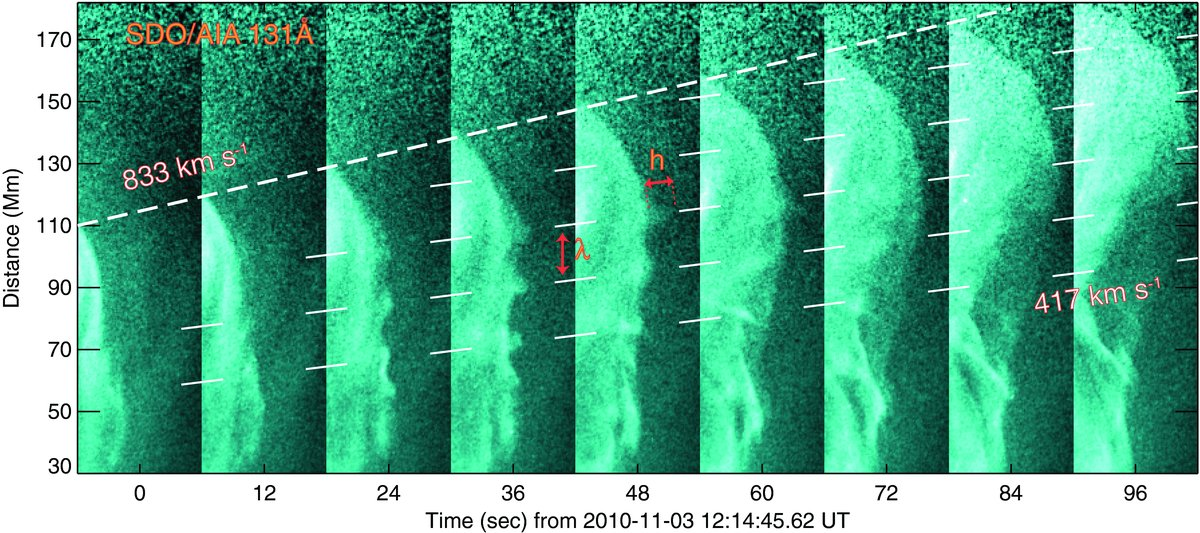
\includegraphics[width=\textwidth]{figures/khi_cme.jpg}
\caption{A time-distance plot of the KHI observed on the flank of a CME in \cite{Foullon2011}.
The parameters $\lambda$ and $h$ correspond to the distance between the KH vortices, and the maximum height of a vortex as measured from the flank, respectively.
}
\label{fig:khicme}
\end{figure}

Of particular interest in this Thesis are the observations of the KHI on the flanks of CMEs (see Figure \ref{fig:khicme}).
It was suggested by \cite{Foullon2011} and \cite{Mostl2013}, that the region on the CME flank where the instability occurs may be modelled as a thin slab in an asymmetric environment.
\cite{Mostl2013} demonstrated that by increasing the strength of the magnetic field on one side of the slab, the KHI on that side is inhibited.
This numerical study shows that exterior asymmetry is an important factor when considering the physics of magnetic slabs.
The observations of \cite{Ofman2011, Foullon2011, Mostl2013} are further discussed in Chapter 2.

\section{Outline of Thesis}

In this Thesis, we study the stability of two MHD configurations subjected to shear flows, and discuss their applications to solar phenomena.
In Chapter 2, we study the steady slab embedded in a static non-magnetic asymmetric environment.
Our analysis starts with the derivation of the governing equations for each section of the system, which was omitted in our discussion of a slab in a symmetric environment in Section \ref{sec:mhdwaves}.
We, then, obtain a dispersion relation for waves propagating along the slab, and some of its approximate solutions.
We solve the dispersion relation numerically to obtain general wave solutions and determine the KHI threshold.
Finally, we discuss how our model may be used for the seismology of KH unstable CMEs.

In Chapter 3, we study an interface separating time-periodic counter streaming flows.
We find that the governing equation for perturbations perpendicular to the interface is Mathieu's equation, and we study its stability.
We discuss our findings in the context of applications to the stability of transverse coronal loop oscillations.

%------------------------------------------------------------------------------
\chapter{Numerical Recipe}
\label{chap:Numerical_Recipe}
%-------------------------------
%------------------------------------------------------------------------------
\section{Brief Overview of Numerical Models}
\label{sec:models}
%------------------------------------------------------------------------------
How these spicules are driven is one of the main issues currently facing solar physicists. The two main avenues of investigation for this phenomenon are observations and numerical simulations. Historically it has been challenging to spatially/temporally resolve spicular structures and the properties on which to base models have been unclear. This has led to a plethora of theoretical models. These models have been reviewed by \cite{Sterling_2000SoPh} and \cite{Aschwanden2019ASSL}, and can broadly be split into the following categories: pressure/velocity pulse in lower/upper chromosphere leading to formation of shocks \citep{Shibata1982,Suematsu1982SoPh7599S,Hollweg1982ApJ257345H,Sterling1990ApJ349647S,Heggland2007ApJ6661277H,kuzma2017ApJ84978K}, p-mode leakage \citep{Pontieu2004Natur},  \Alfven waves which can non-linearly couple and form shocks \citep{Hollweg1982SoPh7535H,Hollweg1992ApJ389731H, Kudoh1999ApJ514493K, Matsumoto2010ApJ7101857M}, magnetic reconnection \citep{Yokoyama1995Natur37542Y,Yokoyama1996PASJ48353Y, Archontis2005ApJ6351299A, Pontieu2007PASJ,Isobe2008ApJ679L57I,Nishizuka2008ApJ683L83N,Sterling2010ApJ,Gonz2017ApJ,Gonz2018arXiv180704224G,Gonz2018ApJ856176G}, joule heating due to ion-neutral collisional dampening \citep{Haerendel1992Natur360241H,James2003AA}, MHD kink waves \citep{Kukhianidze2006AA}, and vortical flows which lead to torsional \Alfven waves that drives spicules \citep{Iijima2017ApJ,Samanta2019Sci}. \np
%
It is important to note that the goal of this thesis is not to determine the origins of spicules. We are interested in the dynamics and morphology of the jet once it is initiated. For this reason, we decided to establish a method of applying a pulse based, driver and we will give a brief overview of the dynamics of these types of models. 
%------------------------------------------------------------------------------
\subsection{Pulse models}
\label{ssec:pulse_model}
%------------------------------------------------------------------------------
Pulse model simulations start with a form of energy deposition in the photosphere or chromosphere that drives material upwards from these regions into the corona. These types of numerical simulations originated in the 1980s, when \cite{Hollweg1982ApJ257345H} developed the rebound shock model which is triggered with a velocity pulse, \cite{Suematsu1982SoPh7599S} placed a pressure pulse in the lower atmosphere, and  \cite{Shibata1982} carried out simulations with pressure pulses in the upper chromosphere. \cite{Sterling_2000SoPh} breaks the velocity pulse into two categories; (i) strong pulse in the lower atmosphere, which covers the photosphere to the low chromosphere, produce initial upward velocities of $\sim 60\kms$ for initial velocities; (ii) weak pulse in the lower atmosphere i.e. the rebound shock model, which has upward velocities in the range of $\sim 1 \kms$. \np
%
\cite{Hollweg1982ApJ257345H} takes a weak pulse of $1\kms$ which is similar to velocities of granular motions at the base of his simulations. Due to the increasing temperature profile of the solar atmosphere, any waves created by disturbing the atmosphere are steepened as they travel upwards. When a wave steepens enough it can form a shock, which lifts the local material. When this lifted, material falls back due to gravity and compresses the lower atmosphere triggering a new wave, which can propagate upwards and steepen, triggering more rebound shocks. \cite{Hollweg1982ApJ257345H} tried to use this model to explain the formation of spicules as the opposing forces exerted by rebound shocks and gravity, cause the TR to undulate, which he interprets as spicules. \cite{Hollweg1982ApJ257345H} shows this model meets some of the characteristics of spicules as the motion of TR could appear as non-ballistic, with comparable mean upward velocities, heights, temperature, and density. Numerous models have built upon rebound shock model, by including radiation and heat conduction \citep{Sterling1988ApJ327950S, Sterling1990ApJ349647S, Cheng1992AA266549C, Cheng1992AA262581C, Cheng1992AA266537C}. With the inclusion of more sophisticated physics it becomes challenging to reproduce spicule characteristics. For example, when \cite{Sterling1990ApJ349647S} added realistic radiation losses, they were not able to produce spicule heights greater than $6~\rm{Mm}$. \cite{Cheng1992AA266549C, Cheng1992AA266537C} used both radiation losses and ionization. He found the only way of generating jets with properties similar to spicules was by having a longer driving time. Recent simulations carried out by \cite{Heggland2007ApJ6661277H} used longer driving times. They showed how to produce chromospheric jets in which radiation losses and ionization could be considered, by placing a monochromatic piston driver at the base of the simulation with velocities (driving times) in the range of $0.2-1.1\kms$ (180-360~\rm{s}). \np
%
\cite{Suematsu1982SoPh7599S} carried out a 1D HD numerical experiment using a strong pulse low in a stratified solar atmosphere. These pulses were initiated by enhancing the pressure ($p/p_0=1.1-5.0$, where $p_0$ is local atmospheric pressure) near the base of the simulation in the region of the photosphere to the low chromosphere ($0.00-0.75~\rm{Mm}$), with driving times of $5~\rm{mins}$. These parameters were chosen based on observations of bright points in the chromosphere which are thought to be linked to the presence of spicules \citep{Suematsu1995ApJ, Jess2012ApJ744L5J, Oxley_2020ApJ905168O}. The pressure enhancement leads to the formation of waves that steepen as they travel upwards. When a wave reaches the steep temperature gradient of the TR it produces strong bi-directional shock waves that lift the TR region. The material behind the perturbed TR is interpreted as a spicule. In this model, rebound shock will occur, but the main difference is that, it is the initial pressure pulse itself, not the rebound shock, that lifts the TR. This model can capture parts of the spicule properties, and results in cool spicules (approx. $10^4~\rm{k}$) with a density of $10^{-13}~\rm{g~cm^{-3}}$, and reaching heights of $3.7-14~\rm{Mm}$. Although the average rise velocity of the spicule of 30 km/s  is in the range of observed spicule speeds, in order to reach the upper end of possible spicule heights, the initial velocity of the top of the spicules must be in the range of 50 - 80 km/s, which is the higher limit of observed spicule velocities. These models were further investigated by \cite{Shibata1982SoPh78333S} and \cite{Shibata1982}, who both studied a wider range of pulse strengths ($1.5 \le p/p_0 \le 30$), a wider variety of pulse heights ($0.18-1.92$), placing the TR at different heights TR. In both studies, they find that if the length between the pressure pulse and TR is reduced then this results in shorter spicules. This is because the waves have less distance to traverse, therefore less atmosphere to steepen in, which causes the shocks to be weaker. \np
%
Another location pressure pulse is placed in the upper chromosphere to simulate spicules. The justification for pressure enhancement at these locations can be created as a consequence of magnetic reconnection. An early example of these models was carried out by \cite{Shibata1982}. These were 1D HD simulations used to investigate the properties of surges, excluding radiation and heat conduction. As stated previously, \cite{Shibata1982} took a large range of pulse heights and strengths. They found that depending on the height which the pulse is located, two different types of jet formation can result, referred to as shock tube jet (above middle chromosphere) and crest shock jet (below middle chromosphere). The shock tube jet is when the pulse itself is responsible for lifting the TR, whereas in the crest shock, the TR is lifted due to a slow shock wave created by the pressure pulse. Compared to the other pulse models there seems to be renewed interest in pressure/velocity pulses just below the TR \citep{Murawski2010AA519A8M, Smirnova2016SoPh2913207S, Kuzma2017AA597A133K, kuzma2017ApJ84978K, Singh2019}. These models include more realistic physics for simulating spicules, such as the inclusion of a magnetic field, radiation losses, thermal conduction, and multi-fluid. They are also able to obtain results in the ranges of spicules height, speeds, temperatures, densities, and trajectories. The resurgence in the upper pulse model may be linked to strong interest in magnetic reconnection as a proposed driver for solar jets, including spicules \citep{Yokoyama1995Natur37542Y, Yokoyama1996PASJ48353Y, Pontieu2007PASJ, Gonz2017ApJ, Gonz2018ApJ856176G}.
%--------------------------------------------------------
\section{MPI-AMRVAC}
%--------------------------------------------------------
All the simulations carried out in this thesis use the open source software Message Passing Interface Adaptive Mesh Refinement Versatile Advection Code (MPI-AMRVAC). This software is developed in Fortran 90 parallelized with Message Passing Interface (MPI) \citep{toth1996ApLC34245T,Keppens_2012,Porth_2014,Xia_2017}. The main focus of this software is maintaining conservation laws in shock dominated problems. This is achieved using shock capturing schemes to retain near-conservation for a set of hyperbolic partial differential equations, typical in conservative form,
\begin{equation}\label{AMRVAC_stlye}
\frac{\partial \boldsymbol{U}}{\partial t} + \nabla \cdot \boldsymbol{F}(\boldsymbol{U}) = \boldsymbol{S}_{phys} (\boldsymbol{U}, \partial_{i} \boldsymbol{U}, \partial_i \partial_j \boldsymbol{U},\boldsymbol{x},t) ,
\end{equation}
where $U$ is the set of conserved variables, $F(U)$ the corresponding fluxes, and $S_{phys}$ are the source terms. The source terms are used to add extra physics, such as gravity, diffusion, and viscosity. In our case, the governing MHD equations are solved in their conservative form (including gravity as an additional source term),
\begin{equation} \label{eq1}
\partial_t \rho + \bn \cdot (\bs{v} \rho) = 0,
\end{equation}   
\begin{equation}\label{eq2}
\partial_t (\rho \bs{v})  + \bn \cdot ( \bs{v} \rho \bs{v} - \bs{BB}) + \bn p_{tot} = \rho \bs{g},
\end{equation}
\begin{equation}\label{eq3}
\partial_t e + \bn \cdot (\bs{v} e - \bs{BB}\cdot\bs{v}+\bs{v}p_{tot}) = \rho \bs{g} \cdot \bs{v},
\end{equation}
\begin{equation}\label{eq4}
\partial_t \bs{B} + \bn \cdot (\bs{vB}-\bs{Bv} ) = 0.
\end{equation}
Above is the full system of MHD equations employed in our model, with variables denoted as: time ($t$), mass density ($\rho$), plasma velocity $\bs{v}$, magnetic field ($\bs{B}$). The total pressure ($p_{tot}$) and energy density ($e$) terms are given as,
\begin{equation}
p_{tot} = p+\frac{\bs{B}^2}{2},
\end{equation}
\begin{equation}
e = \frac{p}{\gamma-1}+ \frac{\rho \bs{v}^2+\bs{B}^2}{2},
\end{equation}
where $\gamma=5/3$ denotes the ratio of specific heats. Solar gravitational acceleration is given by,
\begin{equation}
\bs{g}=-\frac{GM_{\odot}}{r^2}\hat{r},
\end{equation}
where $G$ is the gravitational constant and $M_{\odot}$ denotes the solar mass. \np
%
MPI-AMRVAC has been constructed to be a versatile piece of software, arming the user with a multitude of options. This reduces development time as rather than writing bespoke software for each simulation, modules of the code can efficiently be swapped or modified to produce the desired effect, e.g. changing physic modules, spatial/temporal solvers, grid setup and geometry, changing boundary conditions, and writing one's own custom routines.
%-------------------------------------
\subsection{Adaptive Mesh Refinement}
\label{ssec:amr}
%-------------------------------------
One of the main features of MPI-AMRVAC is the adaptive mesh refinement (AMR). Using AMR means that rather than having a static fixed resolution for the entirety of the simulation, we have a dynamical grid that adds/removes grid cells as needed. For example, see the differing mesh in Fig.~\ref{amr_example} from the test case of a hydrodynamic Rayleigh-Taylor Instability (RTI) (see Section~\ref{chap:tilted_jets} for more description of RTI). In this simulation, there is a denser fluid flowing downwards, and areas of highest resolution are located where rapid changes are occurring in the computational domain. In Fig.~\ref{amr_scheme} we can see different levels of AMR being used. For example, cell (3,1) is the level one grid, which is the coarsest resolution initially defined by the user, cells (6,3) and (12,7) are level two and three respectively, with each cell half the size of the previous level. The rules that AMR are allocated and deallocated are;
\begin{itemize}
    \item The AMR can only be one level higher than its neighbouring cells.
    \item If the measured local numerical error is greater (lesser) than the user set threshold, the level of the grid cell is increased (decreased).
\end{itemize}
It is advantageous to use AMR in our simulations as it allows for computationally efficient placement of grid cells to resolve steep gradients, such as the TR and boundaries of the jet, as well as capturing the small scale dynamics.  
%fffffffffffffffffffffffff
\begin{figure}
\centering
\includegraphics[width = \textwidth]{figures/RTI_example.png}
\caption{Example of AMR mesh for RTI. Notice there is an increased number of grid cells around dynamic regions.: \url{http://amrvac.org/md_doc_examples.html}}.
\label{amr_example}
\end{figure}   
%fffffffffffffffffffffffff
This means that one can increase the grid cells in regions of interest (i.e. where smaller scale dynamics are occurring) based on the numerical error without having to increase the resolution of the whole domain, which would be computationally expensive.
\begin{figure}
\centering
\includegraphics[width = \textwidth]{figures/amrpng.png}
\caption{A generic AMR block skeleton from: \url{http://amrvac.org/md_doc_amrstructure.html}}.
\label{amr_scheme}
\end{figure}   
%------------------------------------------------------------------------------
\subsection{Atmospheric Equilibrium}
\label{sec:atmos_equil}
%------------------------------------------------------------------------------
To create synthetic jets, we need to construct a stratified atmosphere similar to solar conditions. We place the TR at $2$ Mm where the temperature smoothly connects an $8000$ K photosphere to $1.5$ MK corona as shown in \fref{atoms_profile}. The temperature of the atmosphere as a function of height is mathematically represented as,   
\begin{equation}\label{te_pro}
T_0(y>0) = T_{ch}+\frac{T_{c} - T_{ch}}{2} \left[ \tanh \left( \frac{y-y_{tr}}{w_{tr}} \right)+1 \right],
\end{equation}
where $y$ is the vertical position, $T_0(0)=T_{ch}=8\times10^3 \ \rm{K}$ ($T_{c}=1.8\times10^6 \ \rm{K}$) is the chromospheric (coronal) temperature and $y_{tr}=2$ Mm ($w_{tr}=0.02$ Mm) is the TR height (width). There is a uniform vertical magnetic, hence $\bs{j} \times \bs{B}=0$ and magnetohydrostatic equilibrium is achieved with,
\begin{equation}
\frac{dp}{dy} = - \rho g.
\end{equation}
Temperature and pressure are related through the ideal gas law,
\begin{equation}
p = \frac{ \rho \rgas T}{M},
\end{equation} 
where $M$ is the mean atomic weight, $T$ is the temperature and $\rgas$ is the universal gas constant. Therefore, one can obtain the $\rho$ and $p$ in the following form,  
\begin{equation}\label{p_pro}
p(y) = p_0 \exp \left( - \int_0^y  \frac{1}{H(y')} dy' \right), 
\end{equation} 
\begin{equation}\label{rho_pro}
\rho(y) = \rho_0 \frac{T_0}{T(y)} \exp \left( \int_0^y \frac{1}{H(y') }dy' \right),
\end{equation}
where $\rho_0$ and $p_0$ are the initial mass density and pressure equilibrium, respectively, at the lower boundary of the computational domain, and the pressure scale heights are given by,
\begin{equation}
H(y) = \frac{\rgas T(y)}{Mg}.
\end{equation}
Using the temperature profile given by \eref{te_pro} and taking $\rho_0 = 2.34e-4\times10^{-4}\;\rm{kg}\;\rm{m^{-3}}$ we constructed pressure and mass density as function of height by means of \eref{p_pro} and \eref{rho_pro}.
%------------------------------------------------------------------------------
\subsection{Grid Setup}
\label{sec:Grid_Setup}
%------------------------------------------------------------------------------
We set the domain size to $50$ Mm $\times$ $30$ Mm with a level one resolution of $32$ $\times$ $24$ (giving a physical resolution of $\sim$ $1.56$ Mm $\times$ $1.25$ Mm). This coarse level one resolution was chosen to allow the dissipation of shocks as they travel towards the boundaries. To accurately capture the sharpness of the TR, we applied 7 levels of AMR giving a spatial resolution of $\sim$ $12$ km$\times$ $10$ km. We used unidirectional grid stretching in the horizontal direction, where from the origin the grid cells change by a constant factor of $1.1$ from cell to cell. Due to the choice of discretisation scheme for the boundary conditions, we employed ghost cells of 2 grid layers encasing the physical domain in each direction, which have a physical size of $3~\rm{Mm}$. The numerical scheme applied for spatial discretisation is HLL (Harten-Lax-van Leer) \cite{hll_1983} and a third order \u{C}ada limiter \citep{CADA20094118} for the time discretisation. We used the Courant–Friedrichs–Lewy (CFL) number of $0.8$ and generalized Lagrangian multiplier (GLM)-MHD method to maintain $\bs{\nabla} \cdot \bs{B}=0$ \citep{DEDNER2002645}. For the left and right boundary, we utilised a periodic boundary condition. In the ghost cells of the lower boundary, we fixed $\rho$, $e$ and $\bs{B}$ to their initial values. In the ghost cells for the upper boundary the values for $\rho$, $e$ are determined by the gravitational stratification, and $\bs{B}$ was extrapolated assuming zero normal gradient. For both upper and lower boundaries, we took an antisymmetric boundary for the velocity components.
%fffffffffffffffffffffff
\mfig{1}{figures/numerical_Setup_lowres.png}{The top left plot displays an example of the grid at $t=0$. The top right plot shows initial temperature (red line) and density (blue dashed) stratification in the first $10$ Mm. The lower panels from left to right are an example of Gaussian distribution for $A=60$ km s$^{-1}$ and $j_w=187.5$ km marked by red points at $t=0$ and the driver velocity with $A=60$ km s$^{-1}$, $P=300$ s.}{atoms_profile}
%fffffffffffffffffffffffff
%------------------------------------------------------------------------------      
\subsection{Driver}
\label{subsec:driver}
%------------------------------------------------------------------------------
As the driving mechanisms of spicules is an open question, we assumed that the synthetic jet is driven by a momentum pulse from the photosphere to investigate whether simple drivers can recreate the dynamical behaviours of spicules. Rather than going for a pressure pulse, we decided to use a momentum pulse to simulate spicules, as we view spicules as a mass transfer from low heights, since to our knowledge this is yet to be investigated in a solar context. The jet is launched symmetrically by a driver in the centre of the computational domain which varies both spatially and temporally (see bottom panels Fig.~\ref{atoms_profile}). In the $x$-direction the jet velocity is Gaussian with the full width at half maximum (FWHM) of $187.5~\rm{km}$ ($j_w$) and as the jet evolves in time it will reach a switch off phase in which it will shut off with a hyperbolic tangent, as defined by,
\begin{equation}
    v_x(x) = \frac{-A\sin{\theta}}{2}\left( \tanh{\left( \frac{\pi (t-P)}{P}+ \pi \right) +1 } \right) \exp \left( - \left(\frac{x-x_0}{\Delta x} \right)^2  \right),
\end{equation}
\begin{equation}
    v_y(x) = \frac{-A\cos{\theta}}{2}\left( \tanh{\left( \frac{\pi (t-P)}{P}+ \pi \right) +1 } \right) \exp \left( - \left(\frac{x-x_0}{\Delta x} \right)^2  \right),
\end{equation}
where $A$ is the amplitude of the driver, $\theta$ is the tilt angle from the vertical, $P$ are the driver time, $t$ is time, $x$ is horizontal position, $x_0$ location of the central jet axis, $\theta$ is the launching angles, and the $\Delta x$ is based on FWHM of the jet width and is given by,
\begin{equation}
\Delta x = \dfrac{j_w}{2 \sqrt{2 \log{2}}},
\end{equation}
where $j_w$ is the jet width.
\chapter{The Dynamics of Field-aligned Jets in the Solar Atmosphere}
\label{chap:sj}
%-------------------------------------------------------------------------------
\let\thefootnote\relax\footnotetext{
%
This chapter is based on the following refereed journal article:
\begin{itemize}[label={}]
\item Mackenzie Dover, F., Sharma, R., Erd\'elyi, R.; Magnetohydrodynamic Simulations of Spicular Jet Propagation Applied to Lower Solar Atmosphere Model, \apj, Volume 913, Issue 1, \url{https://doi.org/10.3847/1538-4357/abefd1}.
\end{itemize}
}
%------------------------------------------------------------------------------
\section{Introduction}
\label{sec:c2intro}
%------------------------------------------------------------------------------
The aim of this chapter is to investigate the kinematics and morphology of solar spicular jets under a variety of physical conditions. A peculiar property of the solar atmosphere is that the corona is significantly hotter (approx. $1~\rm{MK}$) than the Sun's surface (approx. $6,500~\rm{K}$), apparently breaking the 2nd law of thermodynamics. This ``coronal heating problem" was discovered by \cite{Grotrian1939} and \cite{Edl1943} when they realized that a wrongly acclimated new element, coronium, was in fact high levels of ionization of iron, which would only be possible under extreme temperatures. More recently, the appropriateness of the term ``coronal heating problem" has been called into question by \cite{Aschwanden2007ApJ}, who state that it is a ``paradoxical misnomer", as there is no evidence of local heating in the corona itself, but rather heating occurs in the TR and upper chromosphere. Essentially, the focus for solving the heating of the solar atmosphere should be shifted to instead solve the chromospheric heating problem, and the way in which heat is transported from these regions into the upper solar atmosphere. Spicular jets are a strong candidate to resolve this problem \citep{Kudoh1999ApJ514493K, Pontieu2007PASJ, Martinez-Sykora2017,Moore2011ApJ731L18M, Pontieu2017ApJ, Samanta2019Sci, Zuo2019AcASn, Bale2019Natur}. The energy flux needed to heat the corona is approximately $3\times10^{5}~\rm{erg~cm^{-2}~s^{-1}}$ \citep{Withbroe1977ARAA15363W}. The esitmated energy flux hypthesised for spicules ranges from $\sim 1\times10^5-10^9~\rm{erg~cm^{-2}~s^{-1}}$  \citep{Athay1982ApJ255743A,Zaqarashvili_2009SSRv,Pontieu2011Sci} and with an estimated $2 \times 10^{7}$ \citep{Judge_2010ApJ} Ca II spicules on the Sun's surface at any time, only a small fraction of this energy flux needs to be extracted from a single spicule to maintain the energy budget of the solar atmosphere. \np
%
The Sun's magnetic field is omnipresent throughout the whole solar atmosphere, which dictates the flow and dynamics of plasma. This magnetic field is manifested in numerous thin magnetic flux tubes (MFT), which link the photosphere with the corona and facilitate the transport of mass, energy, and momentum across the TR. Moreover, these MFT structures have the potential to act as conduits for magnetohydrodynamic (MHD) wave modes to propagate from lower solar atmosphere to the corona, and to transfer energy between these regions \citep{Pontieu2004Natur, Kukhianidze2006AA, Zaqarashvili2007A&A, He2009AA497525H}. As outlined in section~\ref{sec:spicule-jets}, due to multiple observed factors; observed wavelengths, physical characteristics (e.g., length, lifetime, velocity), regions (QS, AR or CH), and/or locations (at-limb or on-disk), MFT structures are categorized as different features (e.g., spicules, mottles, dynamic fibrils, macrospicules, x-ray jets, EUV jets, coronal jets) that permeate the solar atmosphere \citep[see reviews by:][]{Beckers1968, Beckers1972ARA&A, Tsiropoula2012}.  In recent years, field-aligned/longitudinal propagation of dominant MHD wave and pulse in MFT structures become has a key focus of research to understand chromospheric heating \citep{Narain1990, Zaqarashvili_2009SSRv, Jess2015}. Understanding the propagation of MHD waves and pulses in a dynamic, gravitationally stratified, inhomogeneous environment can provide vital clues about dissipation mechanisms and the formation of shock-like behaviour associated with thin MFT structures. Observations suggest upward flow velocities in the range $15-110 ~\kms$ for typical lifetimes of between $50-400~\rm{s}$ for off-limb spicular structures (see Table~\ref{solar_jet_table}). The visible apex of these observed features attains a maximum height of approximately $7~\rm{Mm}$ and descends back to the surface following a parabolic trajectory \citep{Pereira2012,Pereira2016ApJ82465P}. \np
%
As highlighted in Section~\ref{sec:models}, many theoretical and numerical approaches have been undertaken to gain an insight into the morphology and dynamical properties of jets in the solar atmosphere. The plethora of models stems from the difficultly constraining parameters with observations and unanswered problems surrounding solar jets: What is their driver? At what height do they originate? What are their typical density, pressure and temperature profiles? Is the same driver responsible for multiple observed jets, or are there multiple ways of driving the same feature? When it comes to the parameterization of solar jets, the picture becomes muddier when considering the relationship between limb and disk features such as TI spicules, mottles, and dynamic fibrils (see Table~\ref{solar_jet_table}). This makes it challenging, from a mathematical modelling perspective, to determine what are the ``correct" parameters on which to base a model. Despite numerous valuable studies, an extensive and qualitative investigation on parameters that influence the observed dynamical characteristics of these spicular features remains missing. In this chapter, we aim to study the propagation of a momentum pulse originating near the photosphere and propagating through the chromosphere and the TR to lower corona in an idealised/stratified solar atmosphere using a simple numerical model. The parameter space comprises driver times, amplitudes, and magnetic field strength, which are examined to assess their role in determining the height, width, and beam structures.
%------------------------------------------------------------------------------     
\section{Parameter Space}
\label{subsec:paramater_space}
%------------------------------------------------------------------------------
Using the numerical setup as described in Chapter~\ref{chap:Numerical_Recipe}, we have conducted numerous simulations to quantify the effects of three key parameters; magnetic field strength ($B$), driver time ($P$), and initial amplitude ($A$) on spicular jet's journey through the solar atmosphere. The parameter space covers the values from $P=50,~200,~300~\rm{s}$, $B_y=20,~40,~60,~80,~100~\rm{G}$, and $A=20,~40,~60,~80~\kms$ to study the impact on jet morphology (maximum height, width and structure) and kinematics (trajectory, transverse displacement). All ranges are based around typical values for classical spicules (see Section \ref{subsec:Spicules} and Table \ref{solar_jet_table}). The driver time is chosen within range of the $5$-minute oscillations of the p-mode \citep{Leighton1962ApJ135474L}, as they are a potential driver for multiple solar features (spicules, mottles  and dynamic fibrils) \citep{Pontieu2004Natur}. In addition, the driver time is based around the measured lifetime of spicular jets (see Table~\ref{solar_jet_table}). The magnetic field strengths are in the range of observed values for spicules, which is consistent with spectropolarimetric estimates for limb spicules \citep{centeno2010, suarez2015}. The range of velocities is chosen based on projectile motion (ignoring drag) to reach spicules' heights. Based on projectile motion, the maximum height for a launching angle of $90^{\circ}$ is,
\begin{equation}
h_{max} = \frac{A^2}{2g}
\end{equation}
where $A$ is initial amplitude, $g=0.274~\rm{km~s^{-2}}$ is solar gravity. For $A=20-80~\rm{km s^{-1}}$, corresponds to $h_{max}=0.73-11.6~\rm{Mm}$. These values fall in the range of observed speeds (heights) seen in spicular jets which have a range of $10-150\kms$ ($0.4-12~\rm{Mm}$) (see table \ref{solar_jet_table}).\textbf{ For TI spicule velocity of $80\kms$ is quite high and typically observed for reconnection jets. Despite this we include this high value in parameter scan to cover a large range of values and to seen what theoretically occurs for a spicule jet nearer the top end of observed velocities.} The magnetic field estimates are consistent with reported magnitudes from spectropolarimetric studies for off-limb spicules \citep{centeno2010, suarez2015}.
\begin{figure}
\centering
{\includegraphics[width=0.4\linewidth]{figures/jet_P300_B60A_60T_0103.png}}
\caption{Example of jet tracking software that accurately estimates height and cross-sectional width parameters for the simulated jet structure. The jet-apex is marked with a yellow triangle with blue dots on jet edges providing an estimate of widths for each height during different evolutionary phases (rise/fall) of the jet.  This figure is available as an animation: \url{https://drive.google.com/file/d/1AJKqjWBShuHm-RwgXHoUjclCRrFSEMZK/view?usp=sharing}}
\label{jet_tracker}
\end{figure}
% may include a summarry table in the intro that is used in presenations, then we could refere to it in text.
% to lift near photospheric mass ($2.34\times10^{-4}~\rm{kg~m^{-3}}$)
%-------------------------
\subsection{Jet Tracking}
\label{subsec:jet_tracking}
%--------------------
To understand the jet dynamics, speed, lifetime, trajectory and jet boundary deformation are measured and compared with observational studies. This is achieved by temporally tracking the jet's width (solid blue dots) and apex (yellow triangle), using jet tracking software (see \fref{jet_tracker}). The jet tracking software developed for this thesis uses the tracer quantity first introduced in MPI-AMRVAC by \cite{Porth_2014}. In essence, the tracer is a non-physical quantity, akin to dye injections, which tracks the advection of a selected area of a fluid (in our case flow entering the computational domain). The injected jet material is given a high arbitrary value of $100$ (jet value), while the ambient environment is set to $0$, and using a threshold of $15\%$, any snapshot can be split into cells belonging to the jet and ambient medium. This is converted into a binary array where $1$ belongs to jet cells and $0$ is the ambient medium, which facilitates easy edge detection. The CSW are estimated as a function of the distance between the opposite jet cells at edges, taken from a horizontal slice across the simulated jet at specified heights (see blue dots in fig.~\ref{jet_tracker}). By having a high resolution with temporal tracking of edges it is possible to obtain useful information of the jet boundary, such as the evolution of boundary deformation at multiple heights. Furthermore, the visible apex of the jet is selected as the highest index of a jet cell in the simulation, which allows us to track the jet's trajectory, speed, acceleration and deceleration (see a yellow triangle in Fig.~\ref{jet_tracker}).
%---------------------------
\subsection{Jet Trajectories}
\label{subsec:jet_traj}
%------------------------
The identified apex of the simulated jets shows a parabolic motion over time, as shown in Fig. \ref{jet_traj}. The estimated jet trajectories reveal non-ballistic paths of the apex, which is consistent with reported observations \citep{Hansteen2006ApJ, Rouppe2007ApJ660L169R, Pontieu2007PASJ} for chromospheric jets. In the numerical setup, the minimum amplitude for the driver is estimated to be $>20 ~\rm{km ~s^{-1}}$ for the near-photospheric plasma to attain spicular heights (see Table \ref{solar_jet_table}). Also, for most cases, the maximum apex for the simulated jets was found to be proportional to the driver amplitude. In each panel, there is a subgroup reaching lower heights due to reduced driving time. We find that our jets have an asymmetric parabolic path as reported in \cite{Singh2019}. This could be due to a piling of jet material as the jet begins to fall, as the falling matter will interact with raising matter, slowing the jet's descent.
\begin{figure}
\captionsetup[subfigure]{labelformat=empty}
\centering
\subfloat[]{\includegraphics[width=0.98\linewidth]{figures/jet_traj.png}}
\caption{Plots show the effects of multiple parameter combinations on maximum apex height attained by the numerical jets'. Results for driver amplitudes with magnitude $A = 20$ km s$^{-1}$ (top-left), $A = 40$ km s$^{-1}$ (top-right), $A = 60$ km s$^{-1}$ (bottom-left), and $A = 80$ km s$^{-1}$ (bottom-right) are shown with jet-apex following a parabolic trajectory. Driver period ($P$), magnetic field strength ($B$) and driver amplitude ($A$) have units in sec, Gauss and km s$^{-1}$ respectively. }
\label{jet_traj}
\end{figure}
%-------------------------------------------
\subsection{Effects on Jet Apex and Widths}
\label{subsec:jet_apex_widths}
%----------------------- 
To understand the impact of the key parameters investigated, we compared how each parameter affects the maximum apex height (panels to the left) and average cross-section width (CSW) (panels to the right) of the jet over its entire life cycle, as displayed in \fref{parameter_scan_lines}. Varying the magnetic field strength ($B$) has less impact on the heights reached by the jet as all cases have shallow gradients, most likely due to the flow of the jet being field-aligned. However, it must be noted that any deviation between jet flow and magnetic field direction can affect the apex height of the jet; this particular aspect is investigated in Chapter 3. The driver time ($P$) has a nuanced effect, as there is a slight decrease in height for $p=50~\rm{s}$, but peaks at $P=200$ and $300~\rm{s}$. This suggests that to transport significant mass from lower in the atmosphere, an instantaneous pulse will not be sufficient. There needs to be a sustained driver, which past a threshold value, does not impact heights reached, but is important in the behaviour of the CSW variation. Both previously mentioned parameters are grouped by colours and line styles for $B$ and $P$ scans, which correspond to matching initial amplitudes. It is found that the jet height is most sensitive to initial amplitude ($A$) of the parameters studied. Based on these indications, the jet height is modelled with a power-law function given as,  
\begin{equation}
h_{max} = C A^{n},
\end{equation}
{\color{green}!!P4!! Power-laws are common feature in nature, based on the presented data there appears to be a parabolic trend across the parameter scan. There we wish to fit a function to this data as it can be used to make prediction on the driver or it gives a metric that can be verified observationally.}by collapsing the data by taking an average at each velocity data point and then fitting an optimal curve using least-squares obtaining values of $C= 10^{-2.21}$ and $n= 1.72$ as shown in the bottom left panel in Fig.~\ref{parameter_scan_lines}. The estimates from the power-law suggest a nonlinear relation between apex height and pulse strength, in contrast to the results reported by \citet{Singh2019}, although both results need to be observationally verified. It must also be noted that \citet{Singh2019} used an instant pressure pulse close to the TR as a driver in their simulation, which might not be directly comparable with our investigation. This could be because in this thesis a larger parameter space is investigated, the jets are initiated at a lower atmospheric height, and the jets studied are faster-moving than studied by \citet{Singh2019}. \np 
%
The panels to the right of Fig.~\ref{parameter_scan_lines} shows the effect of the parameter space on the mean CSW. To obtain the mean CSW, it is measured at every $\rm{Mm}$ the jet reaches and the mean value is calculated over the whole life cycle of the jet. Although this is by no means a perfect method, it does give a useful insight into the global deformation of the jet boundary. Our simulations suggest a strong influence of magnetic field strength in determining the widths of the jet structure, with estimated CSW inversely related to the magnetic field magnitudes. This happens because the jet rises through the stratified atmosphere, it has higher internal pressure (as transporting material with lower atmosphere conditions) compared to the ambient medium. This results in expansion of the jet structure and subsequent distortion of the surrounding field. However, in the case of higher magnetic field magnitudes, the jet experiences strong tension forces that result in greater collimation of the jet structure. These results indicate the possibility of lower cross-sectional widths of jet features located near a strong magnetic field environment than those in quiet Sun regions. Another important aspect that influences the jet width is the lifetime of the driver of the jet. The simulations suggest a linear relationship between the driver periods and the jet CSW. This could be due to the long supply of plasma to the jet by a sustained driver resulting in increased CSW. However, the amplitude of the driver had a minimal effect on the width for the jets aligned with radial magnetic fields, although this might not be the case if the jet direction were misaligned with the background magnetic fields.
\begin{figure}
\captionsetup[subfigure]{labelformat=empty}
\centering
\subfloat[]{\includegraphics[width=\linewidth]{figures/test_combine_image_alt.png}}
\caption{Panels compare the effects of different physical parameters (top to bottom: magnetic field strength, driver period, driver amplitude) on the maximum apex height (left) and mean cross-sectional widths (right) for the simulated jet structure. The shaded-region (bottom left) indicates the 1$\sigma$ error for the power law fit (red line) to the parameter scan. It should be noted that driver period ($P$), magnetic field strength ($B$) and driver amplitude ($A$) have units in sec, Gauss and km s$^{-1}$ respectively.}
\label{parameter_scan_lines}
\end{figure}
%------------------------------------------------------------------------
\section{Synthetic Jet Morphology}
%------------------------------------------------------------------------------
Based on typical criteria for jets of supersonic flows the structures of the jet are akin to a heavy under-expanded jet \citep{Norman1982, Edgington-Mitchell2014} as the jet density and pressure are greater than the ambient medium. From the parameter scan, we define a ``standard'' jet as the one that is most reflective of a spicular jet. The standard jet reaches a height of approx. $8~\rm{Mm}$ with a velocity of observed spicules, showing clear boundary deformation, and is suitable middle ground in the range of morphology seen in the parameter scan. This is depicted in Fig.~\ref{standard_jet}, with $P=300~\rm{s}$, $B=60~\rm{G}$ and $A=60~\kms$, where snapshots of the density (a-d), temperature (e-h) and numerical Schlieren (i-l) are shown. \np
%
The numerical Schlieren represents a normalized density gradient magnitude and is defined as follows,
\begin{equation}
   S_{ch} = \exp{\left( -c_0 \left[ \frac{|\boldsymbol{\nabla} \rho|-c_1 |\boldsymbol{\nabla} \rho|_{max}}{c_2 |\boldsymbol{\nabla} \rho|_{max}-c_1|\boldsymbol{\nabla} \rho|_{max}} \right] \right)},
\end{equation}
%------------------------
where $c_0=5$, $c_1=0.05$ and $c_2=-0.001$. It is important to note while the numerical Schlieren is a physically defined quantity, its use in our analysis is purely from a qualitative perspective as it returns a synthetic shadowgraph image. Shadowgraph images are created by pointing a single light source at a fluid flow in a dark room. It is possible to see the flow patterns because any changes in temperature, pressure, or density, change the refraction index, thus the bending of light rays will create dark and bright regions in the image. An important facet of our simulation is related to the field-aligned jet motions (Fig.~\ref{standard_jet}) that show distinct kinematic and morphological characteristics during rising and falling phases in columns (a-b) and (c-d), respectively. In the rise phase (left-panels of Fig.~\ref{standard_jet}), the simulated jet shows complex internal substructures and sausage-like deformation of cross-sectional widths in density (a-d) and Schlieren (i-l) data. However, during the fall phase (columns of c-d of fig.~\ref{standard_jet}), the complex/internal beam substructure ceases due to driver switch-off. At this stage, the boundary deformation is no longer symmetric, though the jet-axis has noticeable transverse displacement. Modification in sausage-like wave properties associated with CSW estimates during rising and falling phases of simulated jets were recently reported by \cite{Dover2020ApJ90572D}, as described in more detail in chapter 4. The temperature profile of the numerical jet suggests periodic distortion in the TR layer over the jet lifetime. The TR deforms as the jet penetrates this layer while generating waves, also known as TR quakes \citep{Scullion2011}. During its entire lifetime, the jet structure remains isothermal/cool without much variation for any combinations of the selected parameters. Without the inclusion of radiative transfer, any significant insight into the potential heating of the solar atmosphere is out of the scope of this research. \np
%------------------------
\begin{figure}
\captionsetup[subfigure]{labelformat=empty}
\centering
\subfloat[]{\includegraphics[width=0.75\linewidth]{figures/sj_jet_rho_Te_sch.png}}
\caption{Panels show snapshots of temporal evolution of the ``standard’’ numerical jet with uniform radial magnetic field in stratified atmosphere with driver period ($P = 300$ sec), magnetic field ($B = 60$ G) and amplitude ($A = 60$ km s$^{-1}$). The density (a-d), temperature (e-h) and Schlieren (i-l) images highlight complex internal substructures of the simulated jet with bright apex, possibly due to high-density concentrations. The temperature (middle) panel indicates the isothermal nature of the jet structure with a colder plasma component from the photospheric layer. This figure is available as an animation that runs for $8~\rm{s}$, covering $t=0.0~\rm{s}$ to $t=429.4~\rm{s}$: \url{https://drive.google.com/file/d/1Bx3RSm7JSqB3VqtfKEXVNaBftuNoUTOO/view?usp=sharing}.}
\label{standard_jet}
\end{figure}
%-----------------------
Figs. \ref{paramter_scan_one} and \ref{paramter_scan_two} showcase the limit cases for the simulated jet with density structure highlighting variations in parameter space in each row for similar time-instance, as shown in fig.~\ref{standard_jet}. The panels (a-d) and (e-h) in Fig~\ref{paramter_scan_one} exhibits the effect of strong ($B = 80~\rm{G}$) and weak ($B = 20~\rm{G}$) magnetic field strengths, respectively. For the strong magnetic field, the jet was found to be more collimated, with higher density mostly concentrated near the apex. In this case, the complex beam structure is less visible, but due to decreased CSW, it increases the number of knots (areas of enhanced density along the central jet axis) present. The sausage-like jet boundary deformation is less prominent when the magnetic field is stronger. In contrast, in the case of the weak magnetic field, the jet is more diffusive as it balloons out in the solar atmosphere, and due to the large CSW, it decreases the number of knots, as only one is observed. This clearly shows that there is a relationship between CSW and the number of knots. These knots are areas of density enhancements which, when the jet ceases to be driven, flow down the jet to create interesting internal dynamics, particularly in the weak magnetic field example (see (e-f) in Fig.~\ref{paramter_scan_one}). Not only are there changes in the jet boundary deformation in the rise and fall phases of the jet, but there are also changes in the jet beam itself, which may be a useful diagnostic for observers when investigating the potential driver for solar jets. \np    
%
Figs. \ref{paramter_scan_one} (i-l) and \ref{paramter_scan_two} (a-d) showcase the effects of high ($A = 80 ~\kms$) and low ($A = 20 ~\kms$) velocity magnitudes on jet morphology. For higher velocity, the simulated jet had an internal substructure similar to the standard jet, but with more knot features at matching time-steps. The jet shows kinking behaviour from j-l, possibly due to initial high velocity in a slender structure which is more susceptible to kink instability. The transversal displacement travels upwards along the jet beam and starts to bunch closer together when the jet reaches its falling phase, which in turn, changes the directions of flow. For both the standard jet and high amplitude, for example at $t = 288 ~\rm{s}$, the internal substructures disappear, indicating a close association between driver time and knots lifetimes. For $A = 20$ km s$^{-1}$ (top panel: \fref{paramter_scan_two}), the simulations suggest that for a lower velocity the jet heights are reduced and there is an absence of any significant substructures. The initial amplitudes show that they are a key factor in the dynamics and morphology of the jet, as they are responsible for the complex internal substructures and the CSW variations. The horizontal dynamics are a particularly important aspect of this research, as numerical simulations of solar jets do not typically report on CSW variation, even though in observations of spicules they are not just vertically dynamic, as solar spicules exhibit complex motions horizontally \citep{Sharma2018ApJ85361S,Antolin2018ApJ85644A}. \np
%
Panels e-f and i-l in Fig.~\ref{paramter_scan_two} highlight the role of driver period for two cases with magnitudes $P = 50$ and $200~\rm{s}$, respectively. In case of shorter driver period ($P = 50 ~\rm{s}$), the jet at $t = 21~\rm{s}$ shows a similar evolutionary trend as for the longer durations ($P = 200$ and $300~\rm{s}$), with a lifetime of around $t = 223~\rm{s}$. For long duration drivers ($P = 200~\rm{s}$ ), jet boundaries are smooth and show no kink-like deformation in the fall-phase. A key difference between the two driver periods is the amount of mass injection in the jet, which has direct implications for the CSW as the less time the driver is given to supply energy, the faster the jet boundary undulates. \np
%--------------------
\begin{figure}
\captionsetup[subfigure]{labelformat=empty}
\centering
\subfloat[]{\includegraphics[width=0.75\linewidth]{figures/den_plot_1.png}}
\caption{Evolution of the synthetic jet with a different combination of magnetic field and driver amplitude parameters, in a stratified solar atmosphere with uniform radial magnetic field. Parameters are varied for the ``standard’’ jet configuration to identify the effects of a particular parameter on jet morphology and kinematics. Panels (top-bottom) show variations with $B = 80$ G (a-d), $B = 20$ G  (e-h) and $A = 80$ km s$^{-1}$ (i-l), respectively. Animation available for each case are presented in the top row: \url{https://drive.google.com/file/d/1lR1woOJRgORGaD0I9GeAo2WmlcJkBt5z/view?usp=sharing} }
\label{paramter_scan_one}
\end{figure}
\begin{figure}
\captionsetup[subfigure]{labelformat=empty}
\centering
\subfloat[]{\includegraphics[width=0.75\linewidth]{figures/den_plot_2.png}}
\caption{Similar to \fref{paramter_scan_one} with panels (top-bottom) highlighting variations with $A = 20$ km s$^{-1}$ (a-d), $P = 200$ (e-h)$,~50$ s (i-l) respectively for ``standard’’ jet configuration. Animation available for each case are presented in the bottom row: \url{https://drive.google.com/file/d/1lR1woOJRgORGaD0I9GeAo2WmlcJkBt5z/view?usp=sharing}}
\label{paramter_scan_two}
\end{figure}
%---------------------
Overall, the results indicate that changing parameters, whether linked to the driver or the environment through which a jet travels, both have a noticeable impact on the dynamics and morphology of the jet. The parameter scan shows the impact of the morphology of the jet and raises an important question about what is driving these solar jets and at what heights. This series of simulations suggest that if the driver is an instant pulse/short driving time would lead to very thin, low-density jets without complex structures. It also predicts that in regions with a strong magnetic field the jets would be thin, but denser. For each simulation shown, it displays the jet heads being the densest part of the jet. Observational evidence for these bright bulb-like substructures at the jet apex was recently reported in a few studies \citep{depontieu2017, srivastava2018NatAs} for chromospheric jets. \citet{depontieu2017} used a combination of 2.5D radiative MHD simulations and observations for spicule structures, and identified bright leading substructures as ``heating fronts". These authors proposed the formation of these regions as a consequence of upward propagating magnetic waves and/or dissipation of electric currents due to ambipolar diffusion between ions and neutrals. \citet{srivastava2018NatAs} reported ubiquitous observations of chromospheric jets with a leading bright apex, trailed by a dark region in running-difference images. They labelled these jets as ``tadpoles" and suggested the role of pseudo-shocks in the formation of these observed bright substructures.

%------------------------------------------------------------------------------     
\subsection{Jet Beam Structure}
\label{subsec:j_beam_struc}
%------------------------------------------------------------------------------
Our simulations revealed a yet to be observed phenomenon for solar jets, as the synthetic jets contain complex beam substructures. Multiple cases with varied driver amplitudes/periods and magnetic field strength (Figs.~\ref{standard_jet} and \ref{paramter_scan_two}), highlighted criss-cross/knot patterns within the jet beam, along with CSW variations. Complex beam structure seems to be a common feature in the nature in jets, for example with astrophysical \citep{van_Putten_1996ApJ467L57V, DeGouveiaDalPino2005, Hada2013ApJ77570H, Cohen2014ApJ787151C, Hervet2017AnA606A103H} and laboratory jets \citep{Menon2010, Edgington-Mitchell2014, Ono2014}. With current resolution limits, these features would be challenging to observe in solar jets. Two possible mechanisms for the presence of the complex beam structures:
\begin{enumerate}
\item{Knots are the manifestation of non-equilibrium pressure forces prominent within and around the jet structure. As the jet raises it to bring plasma from the lower atmosphere, it thereby has a higher pressure than the ambient medium. Thus, initially, the internal jet pressure results in expansion of the jet which is then counter-balanced by the tension forces of the jet. Eventually, the magnetic pressure dominates the internal plasma pressure, and the jet boundary decreases while resulting in compression of the jet structure. Essentially, there is a ``tug of war" occurring between the pressure forces of the jet and the surrounding magnetic field. This process over height and time appears as CSW deformation of the jet, along with the sites of high density/pressure as knots within the jet structure.}
\item{The knot features could be the sites within the jet structure where internal shock waves \citep{Norman1982} become reflected from the jet boundary. If the jet has supersonic velocities  (synthetic jets have Mach numbers are around $\sim$1-3), it can give rise to a myriad of internal substructures due to high velocities.}
\end{enumerate}
Continuing further in the lens of (2), a schematic overview of these beam (sub)structures is given in Fig. \ref{cartoon_jet_waves}, highlighting two main features, osculating jet boundary and criss-cross pattern formation, that are present in supersonic jets. The boundary deformation arises due to non-equilibrium between the pressure of the jet and the ambient medium. The jet expands from the point of origin as the jet pressure is highest, however, the jet repeatedly overshoots equilibrium points due to the effects of the boundary, communicated to the interior by the sound waves, which are travelling more slowly than the supersonic flow of the jet. Hence, the jet goes through a sequence of expansions and contractions. Not only do supersonic flows give a sausage-like boundary deformation, but the areas of low/high pressure/density are out of phase with maximum/minimum CSW of the jet (see fig. \ref{cartoon_jet_waves}). \np 
%
%----------------
\begin{figure}
\captionsetup[subfigure]{labelformat=empty}
\centering
\subfloat[]{\includegraphics[width=0.8\linewidth]{figures/jet_diagram.eps}}
\caption{A cartoon depicting complex internal substructures in a supersonic jet. The cross-sectional width variations due to formation of regions with high and low pressure as a consequence of internal shock waves, are shown. These wave patterns appear as knots in our simulations, highlighting the role of initial velocity of momentum pulse in generating axisymmetric deformation in a jet structure. }
\label{cartoon_jet_waves}
\end{figure}
The knots inside the jet beam are the manifestation of shock waves trapped inside the jet boundaries. An expansion fan (blue dashed lines in Fig.~\ref{cartoon_jet_waves}) forms at the base of the jet due to the difference in pressure between the jet and the ambient atmosphere. This expansion fan causes an outward flow, making the jet enlarge. The Mach lines of the expansion waves reflect off the jet boundary inwards towards the jet centre in the form of compression waves and a compression fan due to pressure continuity (red lines in Fig.~\ref{cartoon_jet_waves}). The compression waves are reflected at a nearly constant angle from the jet boundary, and as this boundary is curved, the Mach lines of the compression waves tend to converge into a conical shock wave before reaching the centre of the jet. This incident shock either goes under a regular reflection or becomes a Mach disk depending on the angle between the incident shock and the central jet axis, for small and large angles respectively (see black lines Fig.~\ref{cartoon_jet_waves}). These shock waves determine the crisscrossing in the jet beam as well as the shape of the knots. As the flow passes through this shock it increases the pressure in the jet. When the reflected shock reaches the jet boundary it forces the boundary outwards, creating an expansion fan and thus allowing the process to be repeated. \np
%
These shock waves explains the formation of stationary knots while the flow is active, along with CSW deformations (which do not have an anti-node), density enhancements and cavities in the jet structure. In addition, this provides a vital clue about the disappearance of the complex beam substructures during the driver’s switch-off phase. In our simulations, the standard jet (Fig.~\ref{standard_jet}) clearly showcase these knots, and their disappearance with the driver switch-off at around $t=288~\rm{s}$. Similar behaviour is evident from \fref{paramter_scan_one} and \fref{paramter_scan_two}. If this substructure can be seen in jet observations then it gives insight into the driving times.
%------------------------------------------------------------------------------
\section{Summary and Discussion}
\label{sec:c2discussion}
%------------------------------------------------------------------------------
In summary, we have used a simple model to study the effect on jet heights and widths when it is driven by a momentum pulse with enough strength to raise near photospheric material to spicules' heights. This approach is taken to focus on the dynamics of the jets across an extensive parameter scan. The main results of this approach are:  
\begin{itemize}
\item{The visible apex of the jet structure followed a non-ballistic parabolic trajectory with heights comparable with observed spicule motions. A parameter scan suggests a strong influence of driver amplitude in determining the longitudinal dynamics of a jet structure.}

\item{Jets emanating from regions with higher background magnetic field magnitudes are more collimated/dense than those originating in quiet Sun conditions.}

\item{First reports of complex internal substructures are formed during the rising phase of a solar jet structure. These knot patterns are possibly formed due to the reflection of internal shock waves at jet boundaries.}

\item{Temperature maps from our simulations reveal periodic distortions of the transition region due to penetration of jet structure at this layer. However, the jet remained isothermal for its entire life for all combinations of initial parameters. For these simulations, it would be difficult to conclude how much heating these jets can provide to the corona. More physics would need to be added (e.g. radiative transfer and inclusions of neutrals), which is out of the scope of the scientific goals.}

\item{Simulated jets in our study show a bright, bulb-like apex, similar to observed cases of chromospheric jets.}
\end{itemize}
Additionally, the morphology of the synthetics jets is sensitive to the parameters covered in these simulations, i.e. magnetic field strength, driver times and initial amplitude. This may lend credence to linking jet-like events such as dynamics fibrils (AR), mottles (QS) and TI spicules (QS), but apparent differences could partly be attributed to different atmospheric/magnetic environment conditions and differences in parameters of the driver. However, more theoretical and observational evidence is required, for example, running a numerical simulation with the same driver, but changing environmental conditions to match those of observed ARs and QS. \np
%
The synthetic jets show interesting internal dynamics in the beam structures, which need to be confirmed observationally. Two possible mechanisms are proposed; (1) ``tug of war" of jet and ambient pressure, or (2) shock waves caused by the supersonic flow. However, the supersonic flow framework explains the beam structures that are created, the reason that there are areas of density enhancements referred to as knots, cavities along the central jet axis, and the boundary deformation. Knots are seen in many jets from large astrophysical jets \citep{van_Putten_1996ApJ467L57V, DeGouveiaDalPino2005, Hada2013ApJ77570H, Cohen2014ApJ787151C, Hervet2017AnA606A103H} to small laboratory jets \citep{Menon2010, Edgington-Mitchell2014, Ono2014}, hence it makes natural sense that knots are present in solar jets if flow speeds and driver times are sufficient. While this has not yet been observed in small scale solar jets, it is likely due to current resolution limits. In Fig.~\ref{degrid}, the impact of resolution in identifying these features is shown. Observationally the highest spatial resolution is achieved by the Swedish Solar Telescope (SST), at around $70-110~\rm{km}$ \citep{Scharmer2003SPIE,Berger2003ApJ}, as shown in panels e-f. It may be possible to identify jet substructures in the foreseeable future with telescopes such as Daniel K. Inouye Solar Telescope (DKIST). DKIST can achieve spatial resolution of approximately $14-60~\rm{km}$ \citep{Rast2020arXiv,Rimmele2020SoPh}, which is represented by panels a-d. By achieving higher observational resolution, it will be possible to confirm these beam structures, and also to make significant leaps forward in our understanding of solar jets. \np
%
As highlighted earlier, the question of what drives the spicular jet is not yet resolved. The presence/absence of complex beam structures, if observationally verified, would be a significant step forward in understanding the nature of the driver of jets. If observed, then, this can be used to measure lifetime drivers and be used to identify whether a jet is in a rising or falling phase. If they are not observed, then this points towards a short pulse event (e.g. magnetic recognition) as the driver. These substructures could give a new window through which to investigate this phenomenon.
%----------------
\begin{figure}
\captionsetup[subfigure]{labelformat=empty}
\centering
\subfloat[]{\includegraphics[width=0.8\linewidth]{figures/res_den_plot.png}}
\caption{Using the same time step as panel (b) in Fig.~\ref{standard_jet}, the density grid has been degraded to give a rough estimate of the appearance of the jet over a range of resolutions. The panels a-d give covers the possible resolution range of DKIST and panels e-f show the resolution in ranges of SST.}
\label{degrid}
\end{figure}
\chapter{The Effects of Non-field Aligned Flow on Spicular-jets}
\label{chap:tilted_jets}
%==============================================================================
\section{Introduction}
\label{sec:c3intro}
%==============================================================================
A basic question one can ask is, do the flows of plasma in the chromosphere trace the magnetic field lines? Often it is assumed that plasma follows the magnetic field lines in the solar atmosphere. The typical length scale for flows on the Sun tend to be large and the magnetic diffusivity is small, which for ideal MHD means that there is a high magnetic Reynolds number (ratio between advection and diffusion). For a perfectly conducting plasma, the magnetic field lines are frozen into the plasma. This means that the plasma flow is channelled along the field lines, but the perpendicular motion of the flow leads to either the magnetic field lines pushing the plasma or being dragged with the plasma. This is the frozen-in condition that is valid for most plasma features in the coronal environment. However, one can question whether this applies to the chromosphere, where gas pressure can play a more important role than in the corona. \cite{delaCruzRodr2011AA527L8D} investigated whether solar chromospheric fibrils or spicular features trace the magnetic fields. In most cases, these dynamic features trace the field lines, but there were a significant number of examples where there was a misalignment between the plasma structure and the magnetic field lines (approx. $40\%$ of a sample of 32). This misalignment in extreme cases can be larger than $45\degs$. The misalignment of magnetic field and spicular jets was studied further numerically by \cite{Mart2016ApJ831L1M} with a 2.5D radiative MHD simulation, which included ion-neutral interaction effects. The results indicate that the majority of the simulated spicules are misaligned with respect to the magnetic field lines. They record misalignment angles up $25\degs$, and in a more extreme case $40\degs$. Even recent simulations of coronal loops have highlighted that misaligned flows could account for observations of dense plasma falling back to the solar surface \citep{Petralia2018AA609A18P}. \np
%
Another aspect to consider is that spicules are typically inclined from the vertical. Some recent studies measure an average incline of $23.4\degs$ with a range of $0-55\degs$ \citep{Pasachoff2009SoPh26059P}. \cite{Tavabi2012JMPh31786T} reported that spicule inclination from the vertical is affected by the regions in which they manifest, e.g. $<20\degs$ in polar regions, approximately $10\degs$ for CHs, and in ARs they can range from $\pm 60\degs$. All these results are in agreement with older studies on the average inclination of spicules, which report inclinations ranging between $19-35 \degs$ \citep{Beckers1968, Mosher1977SoPh53375M, Heristchi1992SoPh14221H, Tsiropoula2012}. \np
%
The aim of this chapter is to investigate what effect misalignment between jet flow and the magnetic field have on the dynamics and morphology of spicules. The steps taken follow a similar pattern to that of Chapter~\ref{chap:sj}, where a parameter scan is undertaken and, using the jet tracking code, the jets' apex and CSW are measured, and density evolution is investigated. 
%=============================================================
\section{Jet Tracking}
\label{sec:tjt}
%=============================================================
%fffffffffffffffff
\mfig{0.5}{figures/better_slit_size_example.png}{Example of widths being increased artificially due to a tilt in flow, where the width is shown by the black line across the orange rectangle. (a) is the width of a straight jet, (b) is the width taken at the same height, but with the tilted flow, and (c) displays the width measures with (a) [(b)] solid [dashed] black line.}{slit_example}
%fffffffffffffffffff
To keep the results comparable over a range of tilted jets, extra steps have been introduced into the jet tracking software. To accurately measure the width of the jet we can no longer take horizontal slits (as done in Section~\ref{subsec:jet_tracking}) as this could artificially alter the width measurements. For example, imagine a rectangle with a slit across it in a fixed position that finishes on the opposite ends (see (a-b) Fig.~\ref{slit_example}); if one rotates this shape as shown in panel (b), the slit would change in size, hence changing the width measurement of the rectangle as displayed in panel (c). In this case, a slit needs to be placed perpendicular to the central axis, of the rectangle to correct this tilt factor. \np
%
Modifications have been made to the jet tracking software to account for this by tracking the central axis (see yellow stars in Fig.~\ref{imporved_j_track_example}). The yellow stars are the midpoints of horizontal slits taken at $0.1~\rm{Mm}$ intervals. To keep the position of the slits consistent, they are placed at every $1~\rm{Mm}$ based on the jet's length, rather than the height (see the green solid lines in Fig.~\ref{imporved_j_track_example}). The slit is placed perpendicular to the angle of the central jet axis determined by the angle between the data point at each megameter of jet length ($j_{ln}$) and its upper neighbour ($j_{ln+1}$). The edges are identified by first converting the tracer into a binary image as outlined in Section~\ref{subsec:jet_tracking}. A region of $1~\rm{Mm}$ by $0.75~\rm{Mm}$, with $j_{ln}$ as the centre point is selected. The values along the slit are interpolated from the grid and then a gradient is taken to identify the edges. If only one edge is found then the search box is increased approximately by $60\times 50~\rm{km}$ (see Fig.~\ref{search_box_j_track_example}) and the process is repeated until 2 edges are found. The solid blue dots in  Fig.~\ref{imporved_j_track_example} show the method of horizontal slits at every $1~\rm{Mm}$ of height as outlined in Section~\ref{subsec:jet_tracking}. The analysis carried out in this chapter shows the measurements of both methods of taking slits. They are referred to as traced slits when correcting for tilt angles, and horizontal slits to match the earlier method.
%=============================================================
\section{Parameter scans}
\label{sec:pscansII}
%=============================================================
%fffffffffffffffff
\mfig{0.3}{figures/jet_P300_B60A_60T_0039.png}{Example of extended jet tracking software for $\theta=10\degs$. Solid blue dots mark the jet edges of the original method and the red solid dot marks the jet's apex. The green solid line corrects for the tilt and represents the data sampled to find the edges (solid red squares). The yellow stars give the central axis of the jet. Animation is available: \url{https://drive.google.com/file/d/1wio9np70eYhTbXQeHIwHztQZJjmNCb1g/view?usp=sharing}.}{imporved_j_track_example}
%fffffffffffffffffff
Based on the results in Chapter~\ref{chap:sj}, two focused parameter spaces (P1 and P2) are carried out to reduce computational cost. The main goal of P1 is to test the trends observed in Chapter~\ref{chap:sj}, and to determine whether they retain, despite the changes in the flow inclination. The range of values used are: lifetimes with $P=300~\rm{s}$, this parameter was found to be less important in determining jet heights over the investigated range, therefore we stick with the standard jet value; initial amplitudes range from $A=20,~40,~60~\kms$, the velocity upper limit matches the standard jet and as $80~\kms$ is near the upper end of observed spicule velocity, it has been omitted; magnetic field strength covers the same range $B=20,~40,~60,~80~\rm{G}$; tilt angles $T=0,5,15^{\circ}$, this range is to show a small tilt and a value closer to typical tilt angles. The purpose of P2 is to study how the trajectories, CSWs and morphology are affected by the tilting angle of the standard jet ($P=300~\rm{s}, ~B=60~\rm{G}, ~A=60~\kms$). A range of tilts $T=0-60^{\circ}$, in increments of $5^{\circ}$ is investigated. Both parameters scans are sumerised in Table~\ref{scan_table}:
\begin{table*}[]
\centering
\caption{Two sets (P1 \& P2) of parameter magnitudes, including driver lifetimes ($P$), velocity amplitude ($A$), magnetic field strength ($B$) and corresponding inclination angles for simulated jet structure.}
\begin{tabular}{l|l|l|l|l}
\hline
Parameter Scan & P [$\rm{s}$] & A [$\kms$] & B [$\rm{G}$]      & $\theta$ [$\degs$]                                 \\ \hline
P1             & 300       & 20, 40, 60     & 20, 40, 60, 80 & 0, 5, 15                                         \\
P2             & 300       & 60             & 60             & 0, 5, 10, \dots, 60
\\ \hline
\end{tabular}
\label{scan_table}
\end{table*}
%\begin{mylist}
%\item  Lifetimes $P=300~\rm{s}$, initial amplitudes $A=20,~40,~60~\kms$, magnetic field strengths $B=20,~40,~60,~80~\rm{G}$ and tilt angles $\sigma=0,5,15^{\circ}$
%\itemp Lifetimes $P=300~\rm{s}$, initial amplitude $A=60~\kms$, magnetic field strength $B=60~\rm{G}$, and range of tilt angles $\theta=0, ~5, ~10, ~15, ~20, ~25, ~30, ~35,$ $~40, 45, ~50, ~55, ~60^{\circ}$.
%\end{mylist}
%
%-----------------------------------
\subsection{Parameter Scan P1}
\label{subsec:pscansII_I}
%-------------------------
%fffffffffffffffff
\mfig{0.65}{figures/example_of_tilt_jet_code.png}{Example of a binary image used for the search area (coloured box) used in the jet tracking. Markers have the same representation as Fig.~\ref{imporved_j_track_example}.}{search_box_j_track_example}
%fffffffffffffffffff
The results of P1 with a horizontal slit are displayed in Fig. ~\ref{p_scan_t_apex}. For each panel, the colour (line style) corresponds to the tilt angle (initial amplitude for top panels or magnetic strength for bottom panels). From the $\theta=0^{\circ}$ data it is clear that in each panel the general trends and groupings are retained. Overall, introducing a tilt into the flow has a subtle effect on jet heights and mean widths. From the relation between maximum heights and magnetic field, the greater the initial amplitude, the more notable the effect the magnetic strength has on reducing apex heights. This trend is seen in the relation between initial amplitude and maximum height, where again, the greater the tilt angle and initial velocity, the more prominent the reduction in height, as the range of values fans out around $A>40~\kms$. For both mean width panels, there is not a clear trend on how the tilt affects this parameter. \np
%
This process is repeated, but using the maximum length in place of the jet apex and using the traced slits for calculating the mean widths. For the maximum length there is a similar trend to that seen in Fig.~\ref{p_scan_t_apex}, where the magnetic field does not have a significant impact on jet lengths (except for $P=300~\rm{s},~A=60~\kms,~T=15^{\circ}$ data), and there is a positive correlation between maximum length and initial amplitude. In the bottom left panel, it is shown that the maximum length varies more for $A>40~\kms$ for increasing tilt angles. In general, it appears that increasing the tilt reduces the length of the jets, because the jet is intersecting the magnetic field, hence the magnetic field provides a resistance to the jet's forward momentum. An exception is in the case of $P=300,~A=20,~T=15$, where the length is increased, which might be due to the combination of a higher velocity jet, with a weaker magnetic field. In this setup the transverse motion would be larger, thus increasing the length, but maintaining a shorter height. The traced slits shows the jets increasingly collimate with the stronger magnetic field (top right panel), and that there is a greater mean width with larger initial amplitudes. The main difference between the traced and horizontal slits is that the traced slits return slightly larger jet widths.\np
%
In Fig.~\ref{p_scan_t_len} the same parameter scan is investigated, but using a traced slit to account for the tilting of the jet. The top left panel shows the effect of maximum length against the magnetic field strength. The magnetic field strength, in most cases, does not affect the maximum length of the jet. For $P=300,~A=60,~T=15$, increasing magnetic field reduces the synthetic jet's length. For the panel in the bottom left, with $A>40 \kms$ the tilt begins to reduce the maximum length of the jet, but it shows that the greater the initial velocity the longer the jet length. The panels on the right show the effects of the mean width against the change in the magnetic field strength, and initial velocity, top and bottom respectively. The top right panel shows that with increasing magnetic field straight there is more collimation of the jet. From the bottom left panel, as the initial amplitude increases the greater the jet CSW. The trends that we have seen in Chapter~\ref{chap:sj} are maintained when the jet is launched at an angle.  \np
%fffffffffffff
\mfig{1}{figures/horizontal_slit_pscan_fixing.png}{Focused parameter scans demonstrate the effect of tilt over a variety of jet configurations. Panels on the left (right) are based on the maximum apex (mean width) of the jet.}{p_scan_t_apex}
%ffffffffffffffff
%
%ffffffffffffffff
\mfig{1}{figures/traced_slit_pscan_fixing.png}{Focused parameter scans shows the effect of tilt over a variety of jet configurations. Panels on the left (right) are based on the maximum length (mean width) of the jet.}{p_scan_t_len}
%ffffffffffffffff
%-----------------------------------
\subsection{Parameter Scan P2}
\label{subsec:pscansII_II}
%-------------------------
For P2, the effect of the tilt on the CSW measurements and the difference in widths measured using both slits are investigated (see Fig.~\ref{width_measure}). This parameter scan gives a clear indication that increasing tilt angle increases the jet CSWs. At $45^{\circ}$ this trend stops, which happens because as the tilt angle increases, the more nebulous the jet becomes. This occurs particularly in the falling phase, when the jet no longer falls as one clearly defined column, thus making it challenging to identify jet boundaries (see (c),(g), and (k) in Fig.~\ref{tj_morph_4}). Both slits display the same trend, but the traced slit (red solid line) consistently measures higher jet widths, which is in agreement with P1. The analogous trends for both slits originate from the method of angle selection for the traced slits. This is due to the tracking of the central axis of the jet being determined by horizontal slits with small intervals. In combination with a small sample of data points being used to determine the tilt angle, this means that the width measurements may not deviate much from the original slit method. It is possible that a different method of identifying the central axis and/or more data points used for angle determination would modify the trend for the traced slits. Overall, even the less sophisticated method currently used is an improvement on the horizontal slit method and gives an accurate measure of the mentioned jet parameters. However, future improvements are outlined in Section~\ref{sect:fut_work}. \np
%ffffffffffffffff
\mfig{1}{figures/mean_w_vs_tilt.png}{Effect of tilt on the mean width measurement, comparing traced slit (red solid line with data markers) and horizontal slit (blue dashed line with data markers).}{width_measure}
%ffffffffffffffff
%%=============================================================
%\section{Jet Trajectory}
%\label{sec:j_traj_t}
%%=============================================================
%The effect of tilt on the jet is studied using P2. 
The apex height and length of the jet are tracked and displayed in the left panel of Fig.~\ref{tilt_effect_traj}. There is a clear trend, in that both the maximum height (solid black marked line) and length (dashed red marked line) are decreased with a tilting angle. The maximum length is larger than height, and the difference widens above $20^{\circ}$. The increased difference between height and length can be attributed to larger transversal displacement with increasing tilt. Both trajectories of the jet (right-hand panels) display a decrease in maximum height/length and a slight decrease in jet lifetimes of about $150~\rm{s}$, over the range of tilt angles. The results indicate that once tilted up to $50^{\circ}$, the trajectories deviate from what is typically seen in spicular jets. A similar pattern is seen when the jet length is tracked, but the trajectory is less smooth. This latter is because the jet is undergoing transverse motion and is constantly changing in length. These results indicate that both the magnetic field and horizontal perturbations could alter the trajectory of the jet. \np 
%
An interesting aspect of the results is that introducing a small tilt in the flow has produced spicules with differing heights and lifetimes. This means that, a spicule generated with similar energy can appear differently due to non-field aligned flows, which with more misalignment causes shorter heights and lifetimes. This latter finding could explain why spicules appear and disappear over a variety of heights. However, unlike the situation with TII spicules, their appearance would be similar to their higher propagating counterparts. It is only in an extreme case of tilt angles (approx. $50^{\circ}$) that the trajectory significantly deviates from a parabolic flight.
%
%ffffffffffffffff
\mfig{1}{figures/combine_L_h_comp.png}{Plots shows the effect of non-field aligned flow on apex (top panels), length (bottom panels) and trajectories (rightmost panels).}{tilt_effect_traj}
%ffffffffffffffff
%------------------------------------------------------------------------------
\subsection{Tilted Jet Morphology}
\label{subsec:steady}
%------------------------------------------------------------------------------
Figs.~\ref{tj_morph_1} to \ref{tj_morph_4} visualise the density evolution for the standard jet at various tilt angles. The first row of Fig.~\ref{tj_morph_1} serves as a reference to the $\theta=0\degs$ jets described in Chapter~\ref{chap:sj}. Note that in Figs.~\ref{tj_morph_1} to~\ref{tj_morph_3} the timesteps selected are the same as in the simulation snapshots in Chapter~\ref{chap:sj}, this is purposefully chosen for comparison. \np
%
An interesting aspect of the simulation is that even for small tilting angles of $5-10^{\circ}$, the morphology of the jet is significantly changed, particularly in the falling phase shown by columns containing panels (c-d). At about $t=253~\rm{s}$ for $5^{\circ}$ and $10^{\circ}$, the jet experiences an instability, causing a kinking motion to travel through the jet beam, giving a whip effect (see panel (g) in Fig.~\ref{tj_morph_1} for aftermath). This whip motion causes significant mixing to occur in the jet beam (see panels (g) and (k) in Fig.~\ref{tj_morph_1}). This is also observed for higher degrees of tilt, but does not cause significant mixing in the jet beam. Another phenomenon observed in jets with higher degrees of tilt ($>20^{\circ}$) is finger-like structures occurring in the down-flow of the jet, both in the jet beam and its right-hand side boundary. Both these dynamics are likely produced by instabilities. In both cases, to determine precisely which instabilities cause these dynamics is not a trivial task and requires further investigation. Despite this, from their appearance and with the data available, it is possible to narrow down to three potential candidates:
\begin{enumerate}
    \item Rayleigh-Taylor instability (RTI) is the instability of an interface between two fluids of differing densities, where the heavy fluid is on top. If this system is subjected to gravity, then any slight perturbation leads the denser fluid to fall through the lighter fluid, forming finger-like structures as shown in Fig.~\ref{RT_example}.
    \item Kelvin-Helmholtz instability (KHI) occurs if there is a velocity shear in a single continuous fluid. The shearing between these two fluids, once above a critical threshold, causes the interface to form vertices; see Fig.~\ref{KHI_example}.    
    \item Dynamic kink instability (DKI) occurs when plasma flows on a curved trajectory. There are two opposing forces acting on the jet; the centripetal force which is trying to destabilise the flow, and the Lorentz force which is acting to stabilise the flow, as shown in Fig.~\ref{DKI_example}. If the flow is super-\Alfvenic then the centripetal force can outweigh the Lorentz force, enhancing the transverse displacement. This instability occurs in HD but is called a kink instability (KI) (not to be confused with MHD KI), which like the DKI is caused by centripetal force in curved flows \citep{Drazin2002ihsbookD}. Note that this instability, is different from an MHD kink instability which arises due to the Lorentz force enhancing kink motion.
\end{enumerate}
%ffffffffffffffffffff
\begin{figure}
\captionsetup[subfigure]{labelformat=empty}
\centering
\subfloat[]{\includegraphics[width=0.6\linewidth]{figures/RT_example.png}}
\caption{Example of the formation of an RT instability at various time steps. These are results from a simulation shown in \cite{Liang2019PhFl31k2104L}. The red-coloured fluid represents a denser fluid than its blue counterpart and gravity is directed downwards leading to the formation of RTI.}
\label{RT_example}
\end{figure}
%ffffffffffffffffffff
From the list of potential instabilities, the two candidates for the whip effect are KHI or DKI. KHI is observed in many instances in nature, e.g. from clouds, waves in the ocean, and Jupiter's eddies \textit{etc.}  They are present in numerous solar features: coronal mass ejections \citep{Foullon2011ApJ729L8F, Foullon2013ApJ767170F}, coronal loops \citep{Barbulescu2019ApJ870108B}, prominences \citep{Berger2010ApJ7161288B, Ryutova2010SoPh26775R}, solar jets \citep{Filippov2015MNRAS4511117F,Li2018NatSR88136L}, and spicules \citep{Kuridze2016ApJ830133K, Antolin2018ApJ85644A}. As there are significant velocity differences between the jet and ambient medium, the interface between these two regions can become KH unstable. This can lead to deformation of the jet boundary and if shearing is strong enough, it can destabilise the jet. However, \cite{Chandrasekhar1961hhsbookC} has shown that a magnetic field aligned with the flow will impede the development of KHI, which is the case of the simulation showcased. Another aspect to consider is that KHI would be localised to the jet boundary, and would not propagate through the jet beam as seen in the simulations. Due to these factors, it is unlikely that KHI is responsible for the whip effect occurring in the simulations. \np 
%%ffffffffffffffffffff
\begin{figure}
\captionsetup[subfigure]{labelformat=empty}
\centering
\subfloat[]{\includegraphics[width=0.8\linewidth]{figures/KHI_example.png}}
\caption{Example of the formation of a KHI taken from \cite{Barbulescu2018SoPh29386B}. Stage (a) shows the interface between two fluids where $U_0$ and $U_1$ are arbitrary flow speeds before they are subject to a perturbation shown in stage (b). In stage (c) the perturbation is enhanced by the flows creating non-linear wave steepening. This leads to stage (d) where a vortex forms, mixing both fluids.}
\label{KHI_example}
\end{figure}
%ffffffffffffffffffff
%------------------------------------
A strong candidate to explain the whip effect is the DKI. \cite{Zaqarashvili2020ApJ893L46Z} proposed a model showing DKI could cause transverse motions in spicules. If a spicule is travelling at an angle (in their case the curve was introduced by considering a vertically expanding flux tube) and the flow is super-Alfv\'{e}nic, then DKI can enhance transverse motions. DKI can explain the presence of the whiplash motion going through the jet. More investigation is needed to understand why at shallow angles of $5-10\degs$, mixing occurs in the falling phase of the jet beam. One possibility is that above $15^{\circ}$ horizontal motion is sufficient to dampen the instability due to the magnetic field. The magnetic field is acting as a brake to the jet flow, i.e. the more tilt, the more impeded the jet will be thereby resulting in smaller up-flows and a reduction in the effect of the DKI. Interestingly, the whip motion can be seen in Fig.~\ref{paramter_scan_one} for $A=80 \kms$, which does not fully fit in with the DKI, because the flow is not on a curved trajectory. \np 
% RTI in proms review paper: https://link.springer.com/article/10.1007/s41614-017-0013-2
Two possible instabilities to account for finger-like structures in the falling phase of the jet for tilts between $20-45\degs$ are RTI and KHI. RTI is hypothesised to form at prominence boundaries \citep{Berger2008ApJ676L89B,Berger2010ApJ7161288B,Hillier2012ApJ746120H,Berger2017ApJ85060B}, but for spicules, there is no strong observational evidence for RTI occurring. Numerical simulations of astrophysical jets have shown that RTI instability can occur at the jet boundary, where the finger-like structures are seen in the perpendicular cross-section with regard to the central jet axis \citep{Toma2017MNRAS4721253T,Matsumoto2017MNRAS4721421M}, and laboratory plasma jets have shown evidence of RTIs \citep{Zhai2016PhPl23c2121Z}. It may be that with a 3D version of the synthetic jet simulation, RTI would form at the boundaries of the jet. The lack of observations of RTI in spicules, and the fact that RTIs would be oriented in the direction of the magnetic field, makes it unlikely that these are responsible for the finger-like structures seen in the simulations. It is more likely to be KHI, as the finger-like patterns form in the falling phase of the jet where there will be an interaction of up and down flowing material, causing increased shearing. The finger-like structures appear near regions of high density, which are located near the edges of the greatest transverse displacement. With higher resolution or less diffusive numerical schemes the KHI could appear as vortices at these locations. \np
%
\begin{figure}
\captionsetup[subfigure]{labelformat=empty}
\centering
\subfloat[]{\includegraphics[width=0.8\linewidth]{figures/DKI.jpg}}
\caption{Cartoon of dynamic kink instability taken from \cite{Zaqarashvili2020ApJ893L46Z}. The blue (red) lines represent the magnetic field (jet). The blue (red) arrow shows the direction for the Lorentz (centripetal) force.}
\label{DKI_example}
\end{figure}
%ffffffffffffffffffff
The tilt has an important impact on the structuring of the beam. The main noticeable difference is the appearance of knots, as seen in columns containing them (b) in Figs.~\ref{tj_morph_1} to~\ref{tj_morph_4}. For tilt $<15\degs$ the knots are denser and deformed, but for higher degrees of the tilt ($> 10^{\circ}$) the knots are no longer easily identified. This would mean only slight horizontal disturbance to the jets would make it even more challenging to identify knots if present in observations. The tilt causes the densest parts of the jet to change from being contained to the head and knots, as seen in Chapter~\ref{chap:sj}, to the edges where the most transversal displacement is. The greater the tilt, the more the edges of transversal displacement become the densest part of the jet, and the rest of the jet beam reduces in density. The column containing panel (d) reaffirms the earlier result that the jet has a lower apex and reduces the jet lifetimes for increasing tilt.
%
%%ffffffffffffffffffff
%\mfig{1}{figures/tj_den_plot_1.png}{Example of the temporal evolution of different tilts angles for jets from $0,~10,~20^{\circ}$ from top to bottom, respectively.}{tj_morph}
%ffffffffffffffffffff
%------------------------------------------------------------------------------
\subsection{Effect of Tilt on Cross-sectional width variation}
\label{subsec:oscillating}
%------------------------------------------------------------------------------
By introducing tilt into the jets, they not only undergo CSW variations but also transverse motions. These are two key dynamical ingredients that need to be captured in spicular models. Spicules are not just vertically dynamic plasma sticks, they display complex motion all through the body of the jet \citep{Sharma2018ApJ85361S}. \np
%
Using the horizontal slits time-distance plots were created at $1-3~\rm{Mm}$ heights (see Figs.~\ref{td_plot_1Mm} to \ref{td_plot_3Mm}), over the range of tilts. From Fig.~\ref{td_plot_1Mm} for $\theta=0^{\circ}$ there are clear sausage-like motions in the CSW variations. It shows that there is a cavity inside the jet, which is due to the process that creates the knots. Even with the smallest tilting angle ($\theta=5\degs$) investigated, it makes substantial changes to the CSW variations of the jet beam. This appears to be the only example where the combination of both CSW variations and transversal displacement can be cleanly observed at this height, as with increasing tilt the sausage-like CSW variations become less noticeable. The main dynamics shift from symmetrically CSW variations, to transversal displacement that reaches up to approximately $1~\rm{Mm}$ in width. For a tilt of $\theta>25\degs$ the most horizontally displaced regions have much denser edges. These could be regions where the material is building up due to the magnetic field redirecting flow as it is perturbed. With increasing amounts of horizontal velocity, the more the jet travels into the magnetic field, hence the jet material collects at turning points creating denser regions at the jet boundary. For the tilted jets, the large scale transverse motions in the simulations are due to the restoring forces of the ambient magnetic field, which are trying to re-establish an equilibrium. Once the tilt passes $\theta=40\degs$, there is less of a clear jet structure. Similar behaviour is seen at $2~\rm{Mm}$ and $3~\rm{Mm}$ (Fig.~\ref{td_plot_2Mm} and \ref{td_plot_3Mm}), where there appears to typically be one-two global sways of the jet during its lifetime. This shows that the wave-like motion propagates throughout the jet. \np
%
The whip motion has been observed in chromospheric jets \citep{Liu2009ApJ707L37L}. In \cite{Liu2009ApJ707L37L}, the observed jet undergoes a transverse disturbance with a whip motion. This jet has length scales (approx. $43.5~\rm{Mm}$), lifetimes (approx. $>1\rm{hr}$), observed speed (approx. $430~\kms$), and proposed origin is magnetic recognition. The whip motion is proposed to be due to the jet being composed of helical threads undergoing untwisting spins, outlined by \cite{Shibata1985PASJ3731S, Shibata1986SoPh103299S} and \cite{Canfield1996ApJ4641016C}. Although the phenomena has very different origins and scale, the overall motion time-distance plots, present in \cite{Liu2009ApJ707L37L}, appear similar to time-distance plots presented in Figs.~\ref{td_plot_1Mm} to~\ref{td_plot_3Mm} that are proposed to be produced by DKI. This whip motion has been shown in simulations of reconnection jets, where material from the chromosphere is ejected by a sling-shot effect due to reconnection and produces a whip motion \citep{Yokoyama1996PASJ48353Y, Kotani2020PASJ7275K}. We do not disagree with these outlined mechanisms, but DKI could be playing a role in the transverse motions. DKI could form as in this reconnection jet scenario there is both curvature and horizontal perturbation to the magnetic field, in addition to a fast flowing jet. \np
%ffffffffffffffffffff
\begin{figure}
\captionsetup[subfigure]{labelformat=empty}
\centering
\subfloat[]{\includegraphics[width=\linewidth]{figures/tj_den_plot_0_5_10.png}}
\caption{Example of the temporal evolution of different tilt angles for jets from $0,~5,~10^{\circ}$ from top to bottom. Animation available where cases a, e, i are in the top row: \url{https://drive.google.com/file/d/1HbVzpsZc2der4BR0ItXUUd4mxXm-nVSD/view?usp=sharing} }
\label{tj_morph_1}
\end{figure}
%ffffffffffffffffffff
\begin{figure}
\captionsetup[subfigure]{labelformat=empty}
\centering
\subfloat[]{\includegraphics[width=\linewidth]{figures/tj_den_plot_15_20_25.png}}
\caption{Example of the temporal evolution of different tilt angles for jets from $15,~20,~25^{\circ}$ from top to bottom. Animation available where cases a, e, i are in the bottom row: \url{https://drive.google.com/file/d/1HbVzpsZc2der4BR0ItXUUd4mxXm-nVSD/view?usp=sharing}}
\label{tj_morph_2}
\end{figure}
%ffffffffffffffffffff
\begin{figure}
\captionsetup[subfigure]{labelformat=empty}
\centering
\subfloat[]{\includegraphics[width=\linewidth]{figures/tj_den_plot_30_35_40.png}}
\caption{Example of the temporal evolution of different tilt angles for jets from $30,~35,~40^{\circ}$ from top to bottom. Animation available where cases a, e, i are in the top row: \url{https://drive.google.com/file/d/1xW6KnMehodIazDxL7j4y2uXM8j2v6nBq/view?usp=sharing}}
\label{tj_morph_3}
\end{figure}
%ffffffffffffffffffff
\begin{figure}
\captionsetup[subfigure]{labelformat=empty}
\centering
\subfloat[]{\includegraphics[width=\linewidth]{figures/tj_den_plot_45_50_55.png}}
\caption{Example of the temporal evolution of different tilt angles for jets from $45,~50,~55^{\circ}$ from top to bottom. Animation available where cases a, e, i are in the bottom row: \url{https://drive.google.com/file/d/1xW6KnMehodIazDxL7j4y2uXM8j2v6nBq/view?usp=sharing}}
\label{tj_morph_4}
\end{figure}
%ffffffffffffffffffff
%fffffffffffffffffffff
\mfig{1}{figures/td_plot_1Mm.png}{Time distant plot with horizontal slit at $1~\rm{Mm}$ for tilt values $0-55^{\circ}$.}{td_plot_1Mm}
%fffffffffffffffffffff
%
\mfig{1}{figures/td_plot_2Mm.png}{Same as fig.~\ref{td_plot_1Mm}, but at $2~\rm{Mm}$.}{td_plot_2Mm}
\mfig{1}{figures/td_plot_3Mm.png}{Same as fig.~\ref{td_plot_1Mm}, but at $3~\rm{Mm}$.}{td_plot_3Mm}
%fffffffffffffffffffff
%============================================================
\section{Summary and Discussion}
\label{sec:sum}
%============================================================
In summary, the model used in Chapter~\ref{chap:sj} has been generalised to produce non field-aligned flows to study its effect on jet heights, widths and density evolution. A simple approach is taken to capture the basic dynamics of the jet across two focused parameter scans. The main results obtained from this Chapter are:   
\begin{itemize}
\item Over the range of the parameter space studied, the tilt led to a reduction in apex height and length of the jet.
\item Knots may be more challenging to observe in solar jets than first proposed in this thesis. Even with small amounts of tilt the clear structure seen in straight jets becomes deformed and more blended into the jet beam. At high inclination angles, it would be unlikely that knots would be observed. 
\item The whip motion in the jet is probably due to DKI, but more analysis of the simulations is required to confirm this. The assumptions and physical set up (e.g. different form of stratification of atmosphere, geometry, and magnetic field configuration) that are used to derive the dispersion relation in \cite{Zaqarashvili2020ApJ893L46Z} are not directly applicable to the synthetic jet. A new dispersion relation would need to be derived and the wave frequency inside the jet would need to be calculated to determine the point at which the onset of DKI occurs. 
%{\bf RE: ??? While can use stability criteria that jets are DKI if $v_j(y)>1.25 V_{Ae}$}, where $V_{Ae}$ is the external \Alfven speed, the assumptions made for this calculation are not fully applicable to the synthetic jets {\color{green}(e.g. does not account for a stratified medium, simulations are in a slab geometric, \textit{etc.})}.
\item By introducing tilt into the jets, they not only undergo CSW variations but also transverse motions. These are two key dynamical ingredients that need to be captured in spicular models. For small tilting angles ($<10\degs$) there is a combination of both CSW and transverse displacement, but for larger tilts the transverse motion dominates.
\end{itemize}
An important result of these simulations is that even a slight misalignment between flow and magnetic field produces noticeable transversal displacement and has major effects on the morphology. \textbf{Another avenue of exploring tilt flow in spicule jets would be to tilt the magnetic field instead of the jet flow itself. This aspect of solar jets have been studied in !!cite papers!!. It produces interesting features as it would change path the jet would take through the atmosphere, i.e it would travel more through the lower parts of the atmosphere and contact the TR at an angle. If flow are fast enough then DKI has been shown to occur so transverse motion would still be an important factor.}\np
%
The first evidence of transverse motion in spicules was identified by \cite{Pasachoff1968SoPh5131P}. The mechanism by which transverse motion arises remains a subject of debate. Several mechanisms have been suggested, including overshooting of convective motions in the photosphere, granular buffeting, rebound shocks, global $p$-mode oscillations, and reconnection near foot point \citep{Roberts1979SoPh6123R, Sterling1988ApJ327950S, Vranjes2008A_A478553V, Jess2012ApJ744L5J, Ebadi2014ApSS35331E}. The interpretation of the bulk motion of spicules has typically been through the framework of MHD waves. Many studies report the transverse motion of spicules are due to MHD kink waves \citep{Kukhianidze2006AA, De_Pontieu2007, Jess2012ApJ744L5J, Ebadi2014ApSS35331E, Tavabi2015AA573A4T, Jafarzadeh2017ApJS2299J}. The increased interest is due to the spicules' potential to transport the energy contained in these waves throughout the lower atmosphere \citep{De_Pontieu2007, He2009ApJ705L217H, Morton2012NatCo31315M, Jess2012ApJ744L5J}.  These transverse motions are clearly an important ingredient in the dynamics of spicules and potentially in maintaining the hot solar atmosphere. Non-field aligned flow gives another mechanism to produce transverse motions. This simple mechanism is likely to occur due to the conditions of the chromosphere (where the flow will not always be aligned with the magnetic field), and the complexity of the Sun’s magnetic field. Regardless of the tilt angle, the synthetic jets undergo $1-2$ sways of transverse motion, which are larger with increasing tilt angles. Even with simple models of jets, this highlights the complexity of the dynamics. Understanding how a common component of tilt affects the appearance of the jet is a key part of interpreting the dynamics of spicules, and this should be a factor included in any model of spicules.
\chapter{Comparing Synthetic Jets to Observations}
\label{cap:obs}
%-------------------------------------------
\let\thefootnote\relax\footnotetext{
%
This chapter is based on the following refereed journal article:
\begin{itemize}[label={}]
\item Dover, F., Sharma, R.,  Kors\'os, M., Erd\'elyi, R., (2020); Signatures of Cross-sectional Width Modulation in Solar Spicules due to Field-aligned Flows, \apj, Volume 905, Issue 1, \url{https://doi.org/10.3847/1538-4357/abc349}
\end{itemize}
}
%-------------------------------------------
\section{Introduction}
%-------------------------------------------
In this Chapter, the aim is to investigate the cross-sectional width (CSW) behaviour of straight jets and compare them with observations of H$\alpha$ spicules. Observations indicate that spicules generally emanate near the inter-granulation lanes and remain subject to MHD stresses at their footpoint. The associated motions, irrespective of whether turbulent or coherent, become channelled through the spicule structure and are reflected in their observed dynamic behaviour. Broadly, spicule kinematics can be categorized into three major domains: radially transverse, field-aligned, and torsional. These have been extensively examined and interpreted in terms of discrete MHD wave modes \citep[see review:][]{Zaqarashvili_2009SSRv}. \np  
%
Since the discovery of standing kink oscillations that cause transverse displacement in solar structures \citep{Aschwanden1999ApJ520880A, Nakariakov1999Sci285862N, Aschwanden2002SoPh20699A}, MHD waves in solar structures have gained much attention \citep{Cally1985AuJPh38825C, Kudoh1999ApJ514493K, Fujimura2009ApJ7021443F, Zaqarashvili_2009SSRv, Kuridze2012, Jess2012ApJ744L5J, Mooroogen2017AA607A46M, Allcock2019FrASS648A}. This is due to their potential to provide estimates that we can not directly measure in solar structures (e.g. magnetic field strength), and because they are thought to carry sufficient energy to heat the corona \citep{Alfv1947MNRAS107211A, Gordon1983ApJ266373G, Poedts2002ESASP505273P, Srivastava2017NatSR743147S}. The first report of kink waves in spicules was by \cite{Kukhianidze2006AA}, and numerous studies have since followed, with the goal of identification and study of transverse (kink and torsional \Alfven) wave modes \citep{De_Pontieu2007, Ebadi2014ApSS35331E, Pascoe2016AA585L6P, Sharma2017, Tiwari2019ApJ876106T}. However, reports of CSW variations have remained elusive, due to current resolution limits for observations of jet-like chromospheric features. The presence of CSW variations in thin MFT structures, as a possible consequence of $m$ = 0 MHD sausage and/or $m$ = 2 fluting modes, was postulated in earlier theoretical studies \citep{Ziegler1997a, Ziegler1997, Ruderman2010}. Observations that report on CSW variations in spicular structures are limited to on-disk fibrils, where concurrent transverse and CSW were reported as coupled kink and sausage modes by \cite{Jess2012ApJ744L5J} and \cite{Morton2012}. Similar observations for CSW, and intensity oscillations in on-disk slender chromospheric fibrils were reported by \citet{Gafeira2017ApJS2297G} and interpreted as MHD sausage wave modes. Moreover, an ensemble of coupled transverse, CSW and axisymmetric torsional motions were reported in off-limb spicules by \citet{Sharma2018ApJ85361S}, which were interpreted as nonlinear kink modes. \np
% {\bf RE: be a bit careful as in a plasma with neutrals present, this may not be fully the case; worth mentioning it, given the popularity of the ubject these days}
Spicules are essentially jet-like features where mass flows along their magnetic field with velocities in the range of $25-100\kms$  \citep{Beckers1972ARA&A, Sterling_2000SoPh, Pereira2012}. These velocities may even have a dominant effect on the waves that are present in spicular jets. Plasma flows will interact with the oscillatory modes of spicules, e.g. periodic motions along or anti-parallel to the bulk motion will be affected differently. Wave motions in steady waveguides have been investigated in the past in a few theoretical studies for different slab and cylindrical geometries \citep{Narayanan1991,nakariakov1995, terrahomem2003, soler2008}. It was concluded that mass flows can generate a shift in frequencies for confined MHD waves and can influence the wave propagation, even causing resonant flow instabilities, depending upon the direction and strength of mass flows. Though possible effects of mass flow on wave periodicities/propagation are known theoretically, they are yet to be observed in highly localised dynamic waveguides such as solar spicules. \np
%
At multiple points through this thesis, there has been a comparison between the simulations and observations. Interesting features that have arisen in the synthetic jets, particularly the CSW variations and the knots. In this Chapter, we aim to focus on these aspects of the observations by comparing the CSW variations in off-limb spicules with the observed dynamical behaviour with synthetic jets, and highlight observed solar features where knots may be present. \np
%-------------------------------------------
\section{Cross-sectional Width Variation in Synthetic jets}
\label{sec:CSW_syn_jet}
%-------------------------------------------
The synthetic jets studied in the thesis capture some of the fundamental dynamics of a chromospheric jet in a stratified atmosphere. Though the momentum-driven simulated jet lacks a few observed complex physical mechanisms, e.g. radiative losses, ambipolar diffusion, and ion-neutral effects, it still models crucial kinematic behaviour, such as longitudinal/field-aligned plasma motions with CSW variations (Fig.~\ref{jet_P300_B50_A60}) in both rising and falling phases of the jet evolution. \np
%
Using the jet tracking code as outlined in Chapter~\ref{chap:sj} the CSW have been measured for a jet with parameters of $\theta =0\degs$, $P=300~\rm{s}$, $B=50~\rm{G}$, and $A=60\kms$ (see Fig.~\ref{jet_P300_B50_A60}). The parameters of these jets are similar to those of the standard jet, and hence display similar dynamics, morphology, lifetimes, knots, and CSW variations. The jets' widths are temporally tracked at multiple heights, where the blue marks measure the widths and yellow triangle locked onto the apex of the jet. The results of the widths for each megameter the jet reaches in the computational domain are displayed in Fig.~\ref{CSW_m_heights}, which also demonstrates that there are oscillatory patterns at each height, except from at $6~\rm{Mm}$. Oscillatory motion is not seen at $6~\rm{Mm}$ due to lack of time which the synthetic jet spends at this height. \np
%
We decided to focus on slit height at $2~\rm{Mm}$ as it can be compared against observations, and because choosing a lower height gives more temporal data to analyse than higher slits. The life of a jet can be separated into two phases; the rising phase, where the jet is being driven and is propagating upward, and the fall phase where the jet is no longer being driven and apex height is decreasing with time. These regions are separated by using the parabolic trajectory and calculating the point at which the gradient switched from positive to negative, i.e. the apex of the trajectory, which is marked temporally by the solid black vertical line in Fig.~\ref{CSW_2m_height}. One striking feature is seen in Fig.~\ref{CSW_2m_height}; to the best of our knowledge we are the first to discover that there are distinct differences in the behaviour of the boundary deformation for the rising (green line) and falling (cyan line) phases of the jet. During the rising phase, the CSW is larger and with only a few undulations,  whereas in the fall phase the CSW are shorter and faster undulations. The blue and orange lines show the quadratic fit used to detrend the rise and fall phases respectively in Section~\ref{sec:CSW_comp}.
%-----------------------
\begin{figure*}
\includegraphics[width=1.0\textwidth]{figures/jet_P300_B50_A60_with_markers.eps}
\caption{Panels showing the temporal evolution of the simulated spicule density structure at four time-steps with apex marked by a yellow triangle. From $121.08-243.88 ~\rm{s}$ ($366.68-489.48~\rm{s}$)  the rising (falling) phase. Locations of tracers edges are also shown as blue dots, which are used to estimate the variations in CSW during rising and falling phases of jet structure.}
\label{jet_P300_B50_A60} 
\end{figure*}

\begin{figure*}
\includegraphics[width=1.0\textwidth]{figures/P300B50A60.png}
\caption{CSW variations over multiple heights for synthetic jet with $P=300~\rm{s}$, $B=50~\rm{G}$ and $A=60\kms$.} 
\label{CSW_m_heights} 
\end{figure*}

\begin{figure*}
\includegraphics[width=1.0\textwidth]{figures/raw_data_P300B50A60.png}
\caption{CSW variation for slit at $2~\rm{Mm}$. The solid vertical black line separates the rise (green line) and fall (cyan line) phases, located at the time where the jet reaches its apex. The blue and orange lines are a quadratic fit used to detrend the data.}  
\label{CSW_2m_height} 
\end{figure*}
%-------------------------------------------
\section{Observations of Cross-sectional Width Variation in Spicules}
\label{sec:CSW_spicules}
%-------------------------------------------
In Section \ref{sec:c2discussion} we have discussed that SST currently offers one of the highest spatial resolution observations of the chromosphere, making it an ideal telescope to use for tracking the widths of such small features as spicules. SST is a ground-based telescope located in La Palma, which has one of the best seeing conditions in the world, placed $2400~\rm{m}$ above sea level. It has a nearly $1~\rm{m}$ sized aperture and uses active optics to minimise data degradation due to Earth's atmospheric conditions. The data captured in this section uses the CRisp Imaging SpectroPolarimeter (CRISP), which covers a wavelength range of $510$ to $860~\rm{nm}$, with a field of view of approximately $43.5\times43.5~\rm{Mm}$, and a pixel size of roughly $43~\rm{km}$. The spectral line selected for observation is H$\alpha$ $(656.3~\rm{nm})$, giving an angular resolution of approximately $95~\rm{km}$. H$\alpha$ can only form in the light spectrum from regions of the Sun that are cool enough for hydrogen to exist in its atomic form, which are the photosphere and chromosphere. It is part of the Balmer series and forms absorption or emission spectra for hydrogen when the electron jumps from or falls to $N=2$, where $N$ is the electron orbital number. The H$\alpha$ line is commonly used for observing chromospheric structures as it reveals many complex structure in the messy chromosphere \citep{Parmenter1966PASP78250P, von1985AA146192V, Nishikawa1988PASJ40613N, Judge2006ASPC354259J, Leenaarts2007AA473625L, Rutten2008ASPC39754R, Jess2012ApJ744L5J, Pereira2016ApJ82465P, Rutten2017AA598A89R}. \np
% {\bf RE: if u want to be nice to ur colleagues in h23, u may add here some of their papers using h-alpha observations}
The spicules' structures presented in Figs.~\ref{fig:spa},~\ref{fig:spb} and~\ref{fig:spc} were identified in observations carried out on AR NOAA AR11504 at 07:15-07:48 UT, June 21, 2012. The identification of the spicules and data processing of these observations was carried out in collaboration with Dr. Sharma; we will outline the steps taken. The AR was scanned using 31 equally spaced line positions with $86~\rm{m\angstrom}$ steps from $-1.376$ to $+1.29~\rm{\AA}$, relative to the line centre, along with the additional $4$ positions in the far blue wing from $-1.376$ to $+2.064~\rm{\AA}$. Following data acquisition, post-processing of data was carried out using the Multi-Object Multi-Frame Blind Deconvolution \citep[MOMFBD;][]{van2005SoPh228191V} image restoration algorithm. Also, standard procedures available in the image pipeline for CRISP data were implemented \citep{2015}, including differential stretching and removal of dark and flat fielding. \np
%
The processed data spans around $30~\rm{mins}$ and a cadence of $7.7~\rm{s}$. Following the Nyquist criterion, the temporal-resolution of the dataset allowed the detection of MHD wave modes with periodicities over $15.4~\rm{s}$. Only three spicules (SP:A, SP:B, and SP:C) were selected as they needed to be a high-intensity structure with the least possible superimposition by any other surrounding features during their visible lifetime in an observed passband. The identified spicules have an average lifetime of $118\pm 17.88~\rm{s}$ measured from the H$\alpha$ line-centre. It is possible their true lifetime is longer, as spicules tend to change temperature during their evolution and therefore evolve through multiple passbands, which measurements by \cite{Pereira2014ApJ} have shown to have lifetimes in the range of $500-800~\rm{s}$. The observed features have an average length of about $3\pm0.36~\rm{Mm}$ with apices reaching up to an average height of $4.83~\rm{Mm}$. \np
%
The CSW of observed spicule features were estimated using the method adopted from \citet{Sharma2018}. A single Gaussian function with linear background is used to fit the intensity profile across the observed spicules and the FWHM is taken as a measure of CSW of the feature. For the selected spicules, the average FWHM of the spicules measured at $2~\rm{Mm}$ is $144.47~\rm{km}$, which is comparable with other observations for off-limb spicules \citep{Sharma2018}. The spicules are resolved as there is a $3.36$ ($1.52$) pixel (angular-resolution) cover, bearing in mind that the intensity values belonging to the spicule will occupy a space larger than the FWHM. This process is outlined in Fig.~\ref{fig:spa}, where panels a1-a4 shows snapshots of the identified spicule where the cyan line is the vertical slit to track field-aligned plasma motions and horizontal yellow slit is placed at $2~\rm{Mm}$ to track the CSW. Panel (b) displays time-distance data captured with across the vertical slits, which are used to estimate the speed of the spicules and allow for the separation of the rise and fall phases. Panel (c) shows the process of calculating the FWHM of the spicule, where the dark (light) shaded region marks the unperturbed (perturbed) width $W_u$ ($W$) during the spicule lifetime measure by the yellow slit. The unperturbed width is fixed individually for each spicule as the average FWHM calculated over its lifetime, and the perturbed width is the FWHM calculated at each time step of the observations. The temporal variations in CSW are calculated with $\delta W = W(t) - W_{u}$ and were used to estimate the periodicities. \np
%
SP:A in Fig.~\ref{fig:spa} is an off-limb spicule that was observed at $-1.032~\angstrom$ from the H$\alpha$ line core with a total lifetime of around $161.7~\rm{s}$. The feature had a physical length of $3.8~\rm{Mm}$ at an inclination of $21.4\degs$ over the observed limb, with apex height reaching a maximum of $5.3~\rm{Mm}$. The longitudinal motions in the Lagrangian frame were analysed to estimate the velocity and duration of rising and falling phases, using a vertical slit (Fig.~\ref{fig:spa} a1–a4) along the axis of spicule structure. The time-distance analysis of the vertical slit suggests a parabolic profile (Fig. \ref{fig:spa}(b)) of mass motions with an average ascending velocity of $\sim$46.9 km/s. The plasma attains the maximum height in about 81 sec and then falls back to the surface with an average velocity of 40.2 km/s. For the observed lifetime, the average/unperturbed CSW estimate (W$_{u}$) for the spicule structure was around $176~\rm{km}$.
%----------------------------------
\begin{figure*}
\includegraphics[width=1.0\textwidth]{figures/fig_sp_a.png}
\caption{Panels (a1) – (a4) show the temporal evolution of candidate spicule feature (SP:A) in the H$\alpha$ passband at four instances, with positions of vertical (cyan) and horizontal (yellow) slits used for the estimation of field-aligned mass flows and CSW respectively. Panel (b) shows the time-distance plot from the vertical slit on the spicule, highlighting the rise- and fall-phases of field-aligned mass flow. The maximum height attained by the visible plasma is marked with the ‘+’ symbol, along with estimated velocities (46.9 km/s, 40.25 km/s). Bottom panel (c) shows an example of Gaussian fit for intensity magnitudes for horizontal slit location (marked as a yellow line on (a1) – (a4)), with error bars, denoting the standard deviation for intensity values. The vertical black line marks the position of the amplitude of Gaussian fit, while shaded-regions mark average/unperturbed width (W$_{u}$) during spicule lifetime and perturbed/instantaneous width (W). This figure is taken from \cite{Dover2020ApJ90572D} and was produced by Dr. Sharma.}
\label{fig:spa} 
\end{figure*}
%-------------------------------
\section{Comparison of Cross-sectional Width Variation in Synthetic Jets and Spicules}
\label{sec:CSW_comp}
%-------------------------------
The CSW estimates from both observation and synthetic jets indicate an oscillatory pattern during the feature’s lifetime. These were further analysed using wavelet transform to understand the nature of periodicities and associated wave physics. The results obtained from this analysis is viewed in the framework of ideal MHD waves, as this is likely how this phenomenon would be interpreted in observations. To identify any significant periodicities, wavelet power spectra (WPS) and the associated global power spectrum (GPS) are constructed using open-source software developed by \cite{Torrence1998}. The default Morlet wavelet profile was employed with a two-$\sigma$ confidence level on CSW estimates from observations (top panels) and synthetic jet (bottom panels) as shown in Fig.~\ref{WL_1}. The wavelet analysis is applied to both the rising and falling phases, as well the full signal. For the synthetic jets, the rise and fall phases are independently detrended with a quadratic polynomial (see Fig~\ref{CSW_2m_height}). A low order polynomial is chosen to avoid over fitting. In addition, the detrended data are smoothed to reduce noise with a moving average with a window size of 15 and 10 for the rising and falling phases, respectively. \np
%
The peak frequencies were identified in the wavelet analysis as spectral magnitudes in WPS with significance levels over unity and higher, highlighted as black contours in Fig.~\ref{WL_1}. The peaks also had GPS over two-$\sigma$ (95\%) confidence levels (orange dashed-line in Fig.~\ref{WL_1}). The wavelet spectra for observed width variations during spicule lifetime suggest a strong spectral density concentration around $17~\rm{s}$ for $5$ cycles. Interestingly, for the simulated jet structure, the WPS indicates the presence of harmonics concentrated around $65~\rm{s}$ and $32~\rm{s}$ for $8$ and $5$ cycles, respectively. The oscillatory behaviour between the rising and falling phase is displayed in the last two columns, respectively It becomes clear with the wavelet analysis that there are remarkable differences in the periodicities of the falling and rising phases for each example (see periodicities in Table~\ref{table:1} and Figs.~\ref{WL_1} to~\ref{fig:spc}). This modulation of frequency could be tied to the change in direction of flow and its relation to gravity from rising (working against gravity) and falling phases (working with gravity). Wavelet transforms for observational width variations indicate approximately $27~\rm{s}$ periodicity for 3 cycles, while a powerful $70~\rm{s}$ periodicity is present in both GPS and WPS of the simulation data. However, there is a noticeable shift towards lower/higher periodicities/frequencies for two out of three of our identified spicule cases (Table \ref{table:1}) during the fall-phase of the plasma flows in the jet structure. The wavelet spectrum for observed width variations shows dominant periodicity at $16~\rm{s}$ for $5$ cycles, while for simulated data there are two strong periods concentrated around $30~\rm{s}$ and $68~\rm{s}$, each persistent for $5$ and $2.5$ cycles. These results are consistent with previous reports for CSW oscillations in on-disk fibrils \citep{Gafeira2017ApJS2297G}. \np
%
An important aspect of our investigation is the confirmation of the first overtone in cross-sectional width periodicities associated with dynamic waveguides in the solar chromosphere.  Earlier studies were able to only identify higher harmonics in static waveguides (e.g., in a coronal loop), with the presence of fundamental and first overtone \citep{verwichte2004, guo2015}. Recently, the presence of a second overtone was also reported for coronal loop observations by \citet{duckenfield2019}, associated with transverse kink oscillations. It must be noted that wave harmonics can provide vital clues regarding plasma and magnetic field characteristics of the waveguide via solar magneto-seismology applications \citep{andries2005,andries2009}. The presence of overtones in jets provides a key tool for chromospheric magneto-seismology. This phenomenon is not limited to this one observation, as shown in Fig.~\ref{fig:spb} and Fig.~\ref{fig:spc}. For a summary of the results and physical properties of all the selected spicules see Table \ref{table:1}. \np 
\begin{figure*}
\includegraphics[width=1.0\textwidth]{figures/fig_3.png}
\caption{Panels showing the results of spectral analysis of cross-sectional width estimates of observed (top) and simulated (bottom) jet structures. Each panel depicts temporal evolution of overall widths (1.1) and subsequent rise- (2.1) and fall-phases (3.1), along with Wavelet Power Spectra (WPS: 1.2, 2.2, 3.2) and Global Power Spectra (GPS: 1.3, 2.3, 3.3) during each phase of the evolution of the jet. Vertical red line in plots (Obs: 1.1 and Sim 1.1) marks the time when the field-aligned plasma attained the apex height. Further, plots (Obs: 1.1, Sim: 3.2) provide clear indication of a second harmonic of the cross-sectional width deformations in the dynamic spicular waveguide. This figure is taken from \cite{Dover2020ApJ90572D} and produced by Dr. Kors\'os and Dr. Sharma.}
\label{WL_1} 
\end{figure*}
%
\begin{figure*}[h]
\begin{centering}
\includegraphics[width=1.0\textwidth]{figures/fig_4.png}
\caption{Details of spicule SP:B are shown, where panels (a-c) show the same analysis carried out as for Fig.~\ref{fig:spa}, and the bottom 2 panels show the corresponding wavelet analysis as done in Fig.~\ref{WL_1}. This figure is taken from \cite{Dover2020ApJ90572D} and was created by Dr. Sharma.}
\label{fig:spb} 
\end{centering}
\end{figure*}
%
\begin{figure*}
\begin{centering}
\includegraphics[width=1.0\textwidth]{figures/fig_5.png}
\caption{Same as Fig.~\ref{fig:spb}, but for spicule SP:C, where panels (a-c) show the same analysis carried out as for Fig.~\ref{fig:spa} and the bottom 2 panels show the corresponding wavelet analysis, as done in Fig.~\ref{WL_1}. This figure is taken from \cite{Dover2020ApJ90572D} and made by Dr. Sharma.}
\label{fig:spc} 
\end{centering}
\end{figure*}

\afterpage{%
\begin{landscape}% Landscape page
\begin{table*}
\caption{Summary of observed physical characteristics of candidate spicule structures along with estimated periodicities during rising, falling and overall phases. Physical and spectral parameters of the synthetic jet structure are also provided for a comparison between observed and simulated case(s).}  
\label{table:1}      
%{\centering} 
\begin{center}
\begin{tabular}{cccccccc}
\hline
Spicule       & Lifetime & Length & Apex-height & Unperturbed Width & \multicolumn{3}{c}{Periodicity (s)} \\ \cline{6-8} 
              & (sec)    & (Mm)   & (Mm)        & (km)              & Rising phase  & Falling phase  & Overall   \\ \hline
SP:A          & 161.7    & 3.8    & 5.3         & 176.0             & 27.0        & 16.0        & 17.0      \\
SP:B          & 92.4     & 2.2    & 4.8         & 134.6             & 22.5        & 27.4        & 24.7      \\
SP:C          & 100.1    & 2.8    & 4.4         & 122.8             & 41.2        & 31.3        & 48.8      \\ \hline
Simulated jet & 471.0      & 8.0    & 8.0         & 187.5             & 70.0        & 30.0 \& 68.0   & 32.0 \& 65.0 \\ \hline
\end{tabular}
\end{center}
\end{table*}
\end{landscape}
}
%-------------------------------------------
\section{Blobs in Solar Jet Observations}
\label{sec:EUV_jets}
%-------------------------------------------
Observing knot structures is challenging due to the current resolution limits, as stated throughout the thesis. However, larger-scale jets occur on the Sun, and if the flow speed is sufficient then it is possible that patterns of the knots may be observed. In a series of studies on coronal jets blobs structures were observed \citep{Zhang2014AA567A11Z, Zhang2016SoPh291859Z, Chen2015ApJ81571C, Chen2017ApJ84054C}.  \np
%
\cite{Zhang2016SoPh291859Z} show multiple observations of blob structures in solar jets. The observations were captured by Extreme-Ultraviolet Imager (EUVI) in the Sun-Earth Connection Coronal and Heliospheric Investigation (SECCHI) \citep{Howard2008SSRv13667H} instruments of the Solar TErrestrial RElations Observatory (STEREO) \citep{Kaiser2005AdSpR361483K} and SDO, using the AIA instrument \citep{Lemen2012SoPh27517L}. The images in Fig.~\ref{fig_brigt_blobs_2} were observed with STEREO-B in $171~\AA$ filter with a spatial resolution of approximately $2320~\rm{km}$ ($\ang{;;3.2}$) and a cadence of $75~\rm{s}$. Two jets (J1 and J2) originate around a coronal bright point (BP1). These are thought to arise due to magnetic reconnection \citep{Priest1994ApJ427459P, Mandrini1996SoPh168115M, Longcope1998ApJ507433L, Santos2007ASTRA329S}, and the jets flow along closed magnetic loops. J2 is particularly interesting as multiple blobs form along with the jet, which is highlighted by the white arrows in panels (f-g). If at the base of the jet there are mixed magnetic polarities, a current sheet forms between the interface of these regions, and perturbation to this system can lead to magnetic reconnection. If an instability forms at this current sheet during reconnection then this can lead to plasmoids (regions of magnetic islands)\citep{Drake2006Natur443553D}. These plasmoids are proposed by \cite{Zhang2016SoPh291859Z} to explain the blobs in their jet observations. Interestingly, the formation of the blobs by magnetic reconnection has been proposed for chromospheric anemone jets \citep{Singh2012ApJ75933S}, alluding that blobs may occur over a range of different scales of jets \citep{Zhang2016SoPh291859Z}.\np 
%If the current sheet is extremely thin a perturbation to this system can cause it to go unstable and cause magnetic reconnection. This creates magnetic flux which goes onto form plasmoids which creates magnetic island \citep{Drake2006Natur443553D}. These plasmoids are proposed by by \cite{Zhang2016SoPh291859Z} to formed by a tearing-mode instability. The formation of the blobs by magnetic reconnection has been proposed for chromospheric anemone jets also \citep{Singh2012ApJ75933S}.  \np 
%ffffffffffffffffffff
\begin{figure*}[h]
\begin{centering}
\includegraphics[width=1.0\textwidth]{figures/Selection_065.png}
\caption{Observations of solar jets on  2014 September 10 taken from \cite{Zhang2016SoPh291859Z}. Panels (a-h) are running difference images in $171~\AA$ show the occurrence of two jets (J1, J2). The white arrows highlight where the bright blob-like structures sit along the jet beam.}
\label{fig_brigt_blobs_2} 
\end{centering}
\end{figure*}
%ffffffffffffffffffff
%
\cite{Chen2015ApJ81571C, Chen2017ApJ84054C} reported multiple jets observed at the western edge of AR 11513 on the 2nd and 3rd of July 2012. In these jets, blobs are seen in the jet beam (see Fig.~\ref{fig_brigt_blobs_alt}). The space-borne observations were captured with SDO using the Atmospheric Imaging Assembly (AIA) instrument. AIA has a spatial resolution of $1088~\rm{km}$ ($\ang{;;1.5}$) and a temporal resolution of $12~\rm{s}$ for the EUV lines shown in Fig.~\ref{fig_brigt_blobs_alt}. The example jet clearly shows blobs, as highlighted by slices 1 and 2 in panel (b). The conditions under which these form are similar to that outlined by \cite{Zhang2014AA567A11Z} and \cite{Zhang2016SoPh291859Z}, as the brightening at the base of the jet has been shown to contain magnetic fields of opposite polarities \citep{Chen2017ApJ84054C}. \np
%
The suggested mechanism of blob formation in \cite{Zhang2016SoPh291859Z} is plausible, but so too is the mechanism put forward in Chapter~\ref{!!?!!} for blobs/knots to form in the jet beam when the flow is sufficient. In Fig~\ref{fig_brigt_blobs_2} jets J1 and J2 have high apparent speeds of $145\pm15\kms$ and $203\pm\kms$ respectively \citep{Zhang2016SoPh291859Z} and the jet in Fig.~\ref{fig_brigt_blobs_alt} is approximately $200\kms$ \citep{Chen2017ApJ84054C}. Based on the results of the simulations in the thesis it is feasible with these high speeds in a coronal environment for the blob formation to be generated/driven by shocks containing waves trapped in a jet beam. To rule out blobs forming due to shocks, one needs to measure the flow rate of the jet. This is because, as demonstrated in Chapter~\ref{!!?!!}, when the driver for the jet switches off, the knots start to fall through the jet and disappear. Therefore, if there is a continuous flow then a shock-based process may be plausible, or if it is a short, burst-like release of energy that produces flow then it is more likely to be due to magnetic reconnection.
\begin{figure*}[h]
\begin{centering}
\includegraphics[width=1.0\textwidth]{figures/Selection_064.png}
\caption{EUV jet observed in the west of AR 11513 on July 2, 2012. Each panel represents different passband observations denoted in the top left-hand corner in units of Angstroms. The bright blobs in the jet beam are most noticeable in $171~\AA$ where the slices are located. This figure and the analysis it encapsulates was produced by Dr. Chen.}
\label{fig_brigt_blobs_alt} 
\end{centering}
\end{figure*}
%STEREO originally constitute of two nearly identical satellites, reffered to as STEREO-A and STEREO-B, although STEREO-B is no longer in operation since 2014.    
% ($131~\AA$, $171~\AA$, $193~\AA$, $211~\AA$, $304~\AA$ and $335~\AA$)
%\begin{figure*}[h]
%\begin{centering}
%\includegraphics[width=1.0\textwidth]{figures/Selection_063.png}
%\caption{EUV jet observed in AR west of AR 11513 on 2012 July 2. From left to right the columns show shows the $171\AA$ line observation of the jet, emission measure of the jet, DEM-weighted average temperature of the jet. The time stamps are in the top right hand corner of the first column. This figure and the analysis it encapsulates was produced by Dr. Chen.}
%\label{fig_brigt_blobs} 
%\end{centering}
%\end{figure*}
%============================================================
\section{Summary and Discussion}
\label{sec:sum}
%============================================================
This Chapter compares the CSW properties of the synthetic jets with three observations of spicules captured with high-resolution CRISP/SST H$\alpha$ data. For both the simulation and observation, wave behaviour is identified by CSW estimates. Wavelet analysis of the CSW shows the effects of plasma flows on estimated periods. The Chapter discusses the possibilities that blob structures in observations of large solar jets could be knots produced by trapped shock waves in the jet. The main conclusions drawn from the results as follows:
\begin{itemize}
    \item{CSW variations are present in both the observed and synthetic jets, which highlight that CSW variations are a fundamental property of spicule jets. Earlier reports interpreted these variations as a consequence of confined sausage waves in chromospheric jet structures, although similar characteristics are also shown by MHD fluting wave modes. Here, for the first time, an alternate explanation is provided in terms of internal shock waves for cross-sectional deformations of chromospheric waveguides. In Chapter~\ref{!!?!!} we demonstrated that this phenomenon occurs over a whole range of jets with vastly different length scales, e.g. from astrophysical to laboratory jets. Therefore, the CSW variations are an intrinsic physical characteristic of jets with fast flow speeds. However, insufficient attention has been paid to this for solar jets, primarily due to observational constraints.}

    \item{Spectral analysis using wavelet transform suggests noticeable modulation in estimated periodicities for the CSW in both observed and synthetic jet structures. In most cases, the CSW variations have a shorter period in the falling phase than the rising phase. Similar effects were reported in the past for changes in linear MHD wave characteristics due to mass flows in theoretical and prominence studies.}

    \item{For the first time, the first overtone in the estimated periodicity is identified in both observed and simulated dynamic chromospheric waveguides (spicules). This could have important implications for chromospheric magneto-seismology, further enabling the estimation of much needed information for the longitudinal plasma and magnetic field for chromospheric jets.}
    
    \item{Knot formation could be an alternative explanation for blob structures reported in larger solar jets.}
\end{itemize}
%
This Chapter indicates the possible coupling between the longitudinal mass motions and CSW variations in spicule structures. Understanding such behaviour is crucial for the accurate estimation of the overall energy budget for atmospheric heating and associated dissipation mechanisms. Furthermore, simulations suggest the formation of knot substructures within the jet beam, prevalent during the rise-phase of plasma density. These substructures were closely linked with the estimated CSW variations in the jet and could be generated due to shock waves. The simulation results should inform observers to be cautious in attributing CSW variation in fast-flowing jets to sausage waves, as there other mechanisms, (e.g. shock waves occurring in supersonic flows) that can display CSW variations. \np
%
For the larger-scale EUV jets, it should be noted that regardless of formation mechanisms of knots in the jet beam, they can occur over a whole range of scales in jets. It is likely that with the increase in spatial observation on the horizon for spicules, it is only a matter of time before knot structures are observed in spicular jets.
%------------------------------------------------------------------------------
\chapter{Conclusion and Future Work}
\label{chap:con_and_fut_work}
%-------------------------------
\section{Conclusion}
\label{sec:con}
%-------------------------------
The thesis aimed to investigate the fundamental dynamics and morphology of spicular jets. We have achieved this through a simple model, which uses a momentum pulse to drive the jets to simulate a transfer of mass in an idealised solar atmosphere and with a vertical uniform magnetic field. We have taken full advantage of MPI-AMRVAC mesh options to simulate the synthetic jets' rising and falling dynamics with a high spatial resolution. \np
%
In Chapter~\ref{chap:sj} vertical launching of the jet was investigated. An extensive parameter space was investigated, which determined that spicule dynamics and morphology are sensitive to the parameters related to the driver (lifetimes and initial amplitude) and magnetic environment (magnetic field strength). The vertical and horizontal evolution of spicules is measured with our own automated jet tracking software. By using the jet tracking software we capture the main observable features of spicules with the synthetic jets, as we obtained similar heights, speeds, widths and trajectories. Despite numerous numerical studies on the subject of spicular jets, few have reported on the CSW variations and fine structures of spicular jets. We report on both of these and find complex fine structures in the jet beam of spicules due to shock waves, which also create symmetrical deformation of the jet boundary. These fine structures are yet to be observed, but we show that higher resolution observations with telescopes such as DKIST may be able to identify these fine structures.  \np
%
In Chapter~\ref{chap:tilted_jets} we continued to study with the same model for launching jets, but explored the effects that misalignment between the direction of the driver and the magnetic field has on the dynamics and morphology of the synthetic jet. The tilt of the synthetic jet flows introduces interesting dynamics that were not seen in Chapter~\ref{chap:sj}. The main result of this study, even with small tilts angles of $5\degs$, there is a significant impact on the appearance of the synthetic jets. In this thesis, we have presented one of the few models that obtained both the transverse and horizontal dynamics of the spicule. An interesting result is that the misaligned flows cause whip motions and redistribution of the densities to the jet edges. We tentatively propose that the whip motions are possibly a consequence of a DKI, but further research is required. Our research highlights the importance of properly tracking the central axis of the jets to obtain accurate jet trajectories and measurements of CSWs. Non-field aligned flows give another possibility for producing transverse motion in spicules. Given the complexity of the structure of the atmosphere that spicules propagate in, we conjecture that it is likely that non-field flow will occur, and it is an important aspect to include in any models of spicules. \np
%
In Chapter~\ref{cap:obs} we revisit the field-aligned jets and compare their properties with H$\alpha$ observations captured by SST. CSW variations are present in both observations and synthetic jets. We perform a wavelet analysis to measure any significant wave periods. One of the main results in this thesis is that we are the first to report differences in the jet boundary deformation when the jet is in its rising or falling phase. Under the wave interpretation, there is frequency modulation in the falling phase of all the jets, with shorter periods in the falling phase in comparison to the rising phase. We propose that this is due to the change in direction of the mass flows of the jet with respect to the waves. In this wave-based framework, the results of the synthetic jets could be interpreted as identifying the fundamental mode and its first overtone of the sausage wave. However, I think that the results for the CSW variations of the synthetic jets highlight that we should be cautious with this interpretation. As described in Chapter~\ref{chap:tilted_jets}, we showed that CSW variations are possible due to supersonic flows. The boundary deformation of the synthetic jets shows no obvious sign of having an antinode which is an expected feature for a wave, and this may indicate CSW variations are not due to waves, but rather a consequence of the supersonic flow. This result should be kept in mind for observers reporting variations of spicule widths, as there may be other phenomena that can account for these motions. \np
%
The numerical study presented here has limitations when compared with the spicules actual nature. To have a closer match with spicules', extra physics would need to be included, such as radiative transfer, heat conduction, and deploying a 3D model. These limitations are mostly addressed in the future work section. Despite this, there is value in studying less complex models, as they gives insight into the fundamental nature of spicules and allow us to more easily unpick the phenomena occurring in the simulations. This thesis highlights the importance of identifying what is driving the jets, as it is the most important factor for determining their dynamics and morphology. We are at the beginning of the next generation of solar telescopes, with mirror sizes approximately four times that of SST, such as DKIST, which recently released the highest resolution image of the Sun's surface to date and allowed us to see features as small as $30~\rm{km}$, and EST, with first light planned in $2026$. When these data become available, we can advance our knowledge of the fine structuring of the spicules and pin down their driving mechanism. This would be a significant step forward and allow us to narrow down the appropriate numerical models from which to simulate spicules. 
%-------------------------------
\section{Future Work}
\label{sect:fut_work}
%-------------------------------
Multiple improvements can be undertaken to build upon the existing work in this thesis. The jet tracking code for the tilted examples could be improved further. Its current weakness is that it relies on horizontal slits to track the central axis. It would be better if one autonomously separated the left and right boundary of the jet, which is not a trivial task. Then, for each boundary, measure a set distance to assign data points to match up with its boundary counterpart. Then, taking the midpoints of these pairs would yield a more accurate position of the central jet axis. Steps that need to be undertaken to integrate numerical simulations with observations are as follows; spicules are 3D objects, therefore with a 2D model we may be missing important dynamics, for example, torsional motions \citep{DePontieu2012}, and in astrophysical jets, RTI can format the boundary in 3D jet simulations for fast moving jets \citep{Matsumoto772L1M}. A 3D simulation would better capture the dynamical motion of the spicules and may yield interesting results for the behaviour of the boundary deformation. All the simulations in this thesis use a simplified solar atmosphere, and it would be more appropriate to base the atmospheric stratification on semi-empirical data such as VALC or the C7 atmospheric model \citep{Vernazza_1981ApJS,Avrett_2008ApJS}. More complex physics could be added; radiative transfer and heat conduction are important to include as they can impact the final height of the spicules \citep{Sterling1990ApJ349647S}. These additional physics are key if we wish to study the synthetic jet's contribution to chromospheric/coronal heating. Carrying out a two-fluid model of the simulation could be another avenue to investigate, as neutrals could play an important role in spicule evolution \citep{kuzma2017ApJ84978K}. Another direction to investigate would be to try different magnetic field configurations. A significant progression would be to see how an expanding flux tube would impact the presence of the knots. One major improvement of the model, particularly useful for comparing to observations, would be to use forward modelling to convert the parameter of the simulation into observables. For example, the FoMo code \citep{Doorsselaere2016FrASS34V} is set up to accept MPI-AMRVAC data structures. Forward modelling would allow for a more concrete comparison to observations, and may allow us to identify potential observational signatures for the jet phenomena simulated throughout the thesis.

%now enable appendix numbering format and include any appendices
%\appendix
%to do

%next line adds the Bibliography to the contents page
\addcontentsline{toc}{chapter}{Bibliography}
%uncomment next line to change bibliography name to references
%\renewcommand{\bibname}{References}
\bibliographystyle{agsm}
\bibliography{references}

\end{document}
